%-----------------------------------------------------------------------------
%
%               Template for sigplanconf LaTeX Class
%
% Name:         sigplanconf-template.tex
%
% Purpose:      A template for sigplanconf.cls, which is a LaTeX 2e class
%               file for SIGPLAN conference proceedings.
%
% Guide:        Refer to "Author's Guide to the ACM SIGPLAN Class,"
%               sigplanconf-guide.pdf
%
% Author:       Paul C. Anagnostopoulos
%               Windfall Software
%               978 371-2316
%               paul@windfall.com
%
% Created:      15 February 2005
%
%-----------------------------------------------------------------------------


\documentclass{llncs}

\newsavebox{\codebox}

% The following \documentclass options may be useful:
%
% 10pt          To set in 10-point type instead of 9-point.
% 11pt          To set in 11-point type instead of 9-point.
% authoryear    To obtain author/year citation style instead of numeric.

\usepackage{lmodern}
\usepackage[T1]{fontenc}
\usepackage{xspace}
\usepackage{graphicx}
\usepackage{slatex}
\usepackage{subfig}
\usepackage{upgreek}
\usepackage{varwidth}
\usepackage{verbatim}
\usepackage{color}
\usepackage{stmaryrd}
\usepackage{amsmath}
\usepackage{amssymb}
\usepackage{amsthm}
\usepackage{amscd}
\usepackage{mathtools}

\usepackage{xparse}
\makeatletter
\NewDocumentCommand{\raisedminus}{m}{%
  \raisebox{0.2em}{$\m@th#1{-}$}%
}
\NewDocumentCommand{\unaryminus}{}{%
  \mathbin{%
    \mathchoice{%
      \raisedminus\scriptstyle
    }{%
      \raisedminus\scriptstyle
    }{%
      \raisedminus\scriptscriptstyle
    }{%
      \raisedminus\scriptscriptstyle
    }%
  }%
}
\makeatother

% Hyperref likes to go last
\usepackage[
    bookmarks=true,
    bookmarksnumbered=true,
    breaklinks=false,
    raiselinks=true,
    pdfborder={0 0 0},
    colorlinks=false,
    plainpages=false,
    ]{hyperref}

% This makes hyperlinks point to the tops of figures, not their captions
\usepackage[all]{hypcap}

%%%%%%%%%%%%%%%%%%%%%%%%%%%%%%%%%%%%%%%%%%%%%%%%%%%%%%%%%%%%%%%%%%%%%%%%%%%%%%%%%%%%%%%%%%%%%%%%%%%%%
% BEGIN SPACE HACKS
%%%%%%%%%%%%%%%%%%%%%%%%%%%%%%%%%%%%%%%%%%%%%%%%%%%%%%%%%%%%%%%%%%%%%%%%%%%%%%%%%%%%%%%%%%%%%%%%%%%%%

%\usepackage{showframe}

\makeatletter
\renewcommand\normalsize{%
   \@setfontsize\normalsize\@@ptsize{14.5pt}%
   \abovedisplayskip 8\p@ \@plus2\p@ \@minus2\p@
   \belowdisplayskip \abovedisplayskip
   \abovedisplayshortskip 4\p@ \@plus2\p@ \@minus2\p@
   \belowdisplayshortskip \abovedisplayshortskip
   \renewcommand\arraystretch{0.65}
}

\renewcommand\small{%
   \@setfontsize\small\@ixpt{12pt}%
   \abovedisplayskip 7\p@ \@plus2\p@ \@minus2\p@
   \belowdisplayskip \abovedisplayskip
   %\abovedisplayshortskip 0\p@
   %\belowdisplayshortskip 0\p@
   %\belowdisplayskip \abovedisplayskip
   \renewcommand\arraystretch{0.9}
}

%\setlength\floatsep       {3pt \@minus 1\p@}
%\setlength\textfloatsep   {12pt \@minus 4\p@}
%\setlength\intextsep      {3pt \@minus 1\p@}
%\setlength\dblfloatsep    {3pt \@minus 1\p@}
%\setlength\dbltextfloatsep{3pt \@minus 1\p@}
\makeatother

\usepackage{enumitem}
\setlist{noitemsep,topsep=2pt}
\setitemize{noitemsep,topsep=2pt}
\setenumerate{noitemsep,topsep=2pt}

\newcommand{\smallmathfont}{\small}

%%%%%%%%%%%%%%%%%%%%%%%%%%%%%%%%%%%%%%%%%%%%%%%%%%%%%%%%%%%%%%%%%%%%%%%%%%%%%%%%%%%%%%%%%%%%%%%%%%%%%
% END SPACE HACKS
%%%%%%%%%%%%%%%%%%%%%%%%%%%%%%%%%%%%%%%%%%%%%%%%%%%%%%%%%%%%%%%%%%%%%%%%%%%%%%%%%%%%%%%%%%%%%%%%%%%%%

% Hide subsections in TOC
\setcounter{tocdepth}{1}

\newcounter{maththing}\numberwithin{section}{chapter}

\theoremstyle{definition}
\newtheorem{example}{Example}[chapter]

\theoremstyle{plain}
\newtheorem{definition}[example]{Definition}
\newtheorem{theorem}[example]{Theorem}
\newtheorem{lemma}[example]{Lemma}
\newtheorem{corollary}[example]{Corollary}

\newcommand\numberthis{\addtocounter{equation}{1}\tag{\theequation}}

% puts a little space between the \hrule and captions
\belowcaptionskip 0.25\baselineskip
\newcommand{\bottomhrule}{\vspace{3pt}\hrule\vspace{3pt}}

% keywords
\newcommand{\keyword}[1]{\textbf{#1}}
\newcommand{\mykeyword}[1]{\textbf{\textit{#1}}}

\newcommand\xqed[1]{%
  \leavevmode\unskip\penalty9999 \hbox{}\nobreak\hfill
  \quad\hbox{#1}}

\newcommand{\exampleqed}{\xqed{$\diamondsuit$}}


\newcommand{\lzfclang}{\ensuremath{\lambda_{\text{ZFC}}}\xspace}

%
% Language phase 0: meta
%
% Mostly semantic functions and grammars, definitional extensions to first-order logic

\newcommand{\metadef}{:=}
\newcommand{\metastx}{:\equiv}
\newcommand{\objdef}{:=}
\newcommand{\objstx}{:\equiv}
\newcommand{\gor}{\ |\ }
\newcommand{\meaningof}[1]{\left\llbracket{#1}\right\rrbracket}
\newcommand{\enc}[1]{\mathcal{F}\!\meaningof{#1}}
\newcommand{\stx}[1]{\mathcal{S}\!\meaningof{#1}}
%\newcommand{\metasubst}[3]{{#1}[{#2}:={#3}]}
\newcommand{\metasubst}[3]{s\!\meaningof{{#1},{#2},{#3}}}
\newcommand{\imp}{\Rightarrow}
\newcommand{\rimp}{\Leftarrow}
\DeclareMathOperator{\disjoint}{\mbox{$\not\mspace{-5mu}\i$}}

\renewcommand{\dots}{...}
\newcommand{\setb}[2]{\lbrace {#1} \ \lvert\ {#2} \rbrace}

\newcommand{\justdenom}[1]{\mspace{-4mu} {} \atop {#1} \mspace{-4mu}}
\newcommand{\djustdenom}[1]{\displaystyle{\justdenom{#1}}}


%
% Language phase 1: first-order logic
%

% Common notation and names

\newcommand{\set}[1]{\{{#1}\}}
\newcommand{\seq}[1]{\left({#1}\right)}
\newcommand{\pair}[1]{\langle{#1}\rangle}
\newcommand{\dpair}[1]{\left\langle{#1}\right\rangle}

\newcommand{\band}{\wedge}
\newcommand{\pand}{\big\wedge}
\newcommand{\bor}{\vee}
\newcommand{\por}{\big\vee}

\newcommand{\Bool}{\mathbb{B}}
\newcommand{\Nat}{\mathbb{N}}
\newcommand{\Int}{\mathbb{Z}}
\newcommand{\Rat}{\mathbb{Q}}
\renewcommand{\Re}{\mathbb{R}}
\renewcommand{\P}{\mathbb{P}}

\newcommand{\U}{\textstyle\bigcup}
\renewcommand{\u}{\cup}
\newcommand{\I}{\textstyle\bigcap}
\renewcommand{\i}{\cap}
\newcommand{\wo}{\backslash}
\let\oldemptyset\emptyset
\renewcommand{\emptyset}{\varnothing}
\newcommand{\powerset}{\mathcal{P}}

\newcommand{\Forall}[1]{\forall\,{#1}\ldotp\,}
\newcommand{\Exists}[1]{\exists\,{#1}\ldotp\,}
\newcommand{\ExistsOne}[1]{\exists\char`^\,{#1}\ldotp\,}
\newcommand{\The}[1]{\iota\,{#1}\ldotp\,}

\newcommand{\tto}{\Rightarrow}
%\newcommand{\bijto}{\xrightarrow{\mathrm{bij}}}
\newcommand{\bijto}{\leftrightarrow}
\newcommand{\Ord}{\mathit{Ord}}

\newcommand{\A}{\mathcal{A}}
\newcommand{\B}{\mathcal{B}}
\newcommand{\C}{\mathcal{C}}
\newcommand{\E}{\mathcal{E}}
\newcommand{\V}{\mathcal{V}}

\newcommand{\pnand}{\mathit{nand}}
\newcommand{\w}{\backslash}

% Invented notation and names

\newcommand{\myfun}[1]{\mathit{#1}}
\newcommand{\encset}{\myfun{set}}
\newcommand{\lex}{\myfun{lex}}
\newcommand{\addset}{\myfun{put}}

%\newcommand{\dto}{\Downarrow}
% makes the horizontal spacing around the arrow nice:
\DeclareMathOperator{\dto}{\Downarrow}

\newcommand{\plusomega}{+_\lnat}
\newcommand{\timesomega}{\times_\lnat}

\newcommand{\plusint}{+_Z}
\newcommand{\minusint}{-_Z}
\newcommand{\timesint}{\times_Z}
\newcommand{\equalint}{=_{\mathsf{Z}}}

\newcommand{\plusz}{+_\Int}
\newcommand{\minusz}{-_\Int}
\newcommand{\timesz}{\times_\Int}

\newcommand{\equalrat}{=_{\mathsf{Q}}}
\newcommand{\plusq}{+_\Rat}
\newcommand{\minusq}{-_\Rat}
\newcommand{\timesq}{\times_\Rat}
\newcommand{\divq}{\div_\Rat}

%
% Language phase 2: lambda_ZFC
%

\newcommand{\objlang}[1]{\mathsf{#1}}
%\newcommand{\objlang}[1]{\mathtt{#1}}

\renewcommand{\choose}{\mathcal{E}}
%\newcommand{\Choose}[1]{\choose\,{#1}\ldotp\,}
\newcommand{\Choose}[1]{\set{#1}\ldotp\,}

\newcommand{\domain}{\objlang{domain}}
\newcommand{\range}{\objlang{range}}
\newcommand{\image}{\objlang{image}}
\newcommand{\filter}{\objlang{select}}

\newcommand{\lunion}[1]{{\textstyle\U}\ {#1}}
\newcommand{\lpowerset}[1]{\powerset\ {#1}}
\newcommand{\limage}[2]{{\objlang{image}}\ {#1}\ {#2}}
\newcommand{\lorder}[1]{{\objlang{card}}\ {#1}}
\newcommand{\ltake}[1]{{\objlang{take}}\ {#1}}
\newcommand{\lemptyset}{\oldemptyset}
\newcommand{\lnat}{\upomega}
\newcommand{\lif}[3]{{\objlang{if}}\ {#1}\ {#2}\ {#3}}
\newcommand{\ltrue}{\objlang{true}}
\newcommand{\lfalse}{\objlang{false}}
\newcommand{\lfun}{\lambda\ldotp\,}

\newcommand{\fun}[1]{\lambda\mspace{2mu}{#1}\ldotp\,}

\newcommand{\tvar}{t_\mathrm{var}}
\newcommand{\tapp}{t_\mathrm{app}}
\newcommand{\tif}{t_\mathrm{if}}
\newcommand{\tin}{t_\in}
\newcommand{\tunion}{t_\u}
\newcommand{\ttake}{t_\mathrm{take}}
\newcommand{\tpowerset}{t_\powerset}
\newcommand{\timage}{t_\mathrm{image}}
\newcommand{\torder}{t_\mathrm{card}}
\newcommand{\tset}{t_\mathrm{set}}
\newcommand{\tatom}{t_\mathrm{atom}}
\newcommand{\tfun}{t_\lambda}
\newcommand{\atrue}{a_\mathrm{true}}
\newcommand{\afalse}{a_\mathrm{false}}
\newcommand{\ttrue}{t_\mathrm{true}}
\newcommand{\tfalse}{t_\mathrm{false}}

\newcommand{\Vatom}{V_\mathrm{atom}}
\newcommand{\Vset}{V_\mathrm{set}}
\newcommand{\Vfun}{V_\lambda}
\newcommand{\Evar}{E_\mathrm{var}}
\newcommand{\Eapp}{E_\mathrm{app}}
\newcommand{\Eset}{E_\mathrm{set}}
\newcommand{\Eif}{E_\mathrm{if}}
\newcommand{\Ein}{E_\in}
\newcommand{\Eunion}{E_\u}
\newcommand{\Epowerset}{E_\powerset}
\newcommand{\Eimage}{E_\mathrm{image}}
\newcommand{\Eorder}{E_\mathrm{card}}

\newcommand{\fst}{\myfun{fst}}
\newcommand{\snd}{\myfun{snd}}

\newcommand{\jand}{\;\;\,}

\newenvironment{displaybreaks}%
{%
	\begingroup%
	\allowdisplaybreaks%
}%
{%
	\endgroup%
	\ignorespacesafterend%
}

%\excludecomment{proof}

\newcommand{\figref}[1]{Fig.~\ref{#1}}
\newcommand{\figsref}[1]{Figs.~\ref{#1}}

\newcommand{\arrow}{\rightsquigarrow}

\newcommand{\restrict}[1]{\lvert_{#1}}
\newcommand{\pto}{\rightharpoonup}
\newcommand{\Un}{\mathcal{U}}

\newcommand{\join}{\vee}

\newcommand{\conv}{^{\mspace{-2mu}\Downarrow\mspace{-2mu}}}

\newcommand{\meaningofconv}[1]{\left\llbracket{#1}\right\rrbracket\conv}

\newcommand{\arrowlift}{\ensuremath{lift}}
\newcommand{\arrowarr}{\ensuremath{arr}}
\newcommand{\arrowcomp}{\ensuremath{{>}\mspace{-6mu}{>}\mspace{-6mu}{>}}}
\newcommand{\arrowpair}{\ensuremath{\mathit{\&\mspace{-7.5mu}\&\mspace{-7.5mu}\&}}}
\newcommand{\arrowif}{\ensuremath{ifte}}
\newcommand{\arrowconvif}{\ensuremath{ifte\conv}}
\newcommand{\arrowlazy}{\ensuremath{lazy}}
\newcommand{\arrowapp}{\ensuremath{app}}
\newcommand{\arrowrun}{\ensuremath{run}}
\newcommand{\arrowget}{\ensuremath{get}}
\newcommand{\arrowerror}{\ensuremath{error}}
\newcommand{\arrowtrans}{\ensuremath{\eta}}

\newcommand{\gen}{_\mathrm{a}}
\newcommand{\genb}{_\mathrm{b}}
\newcommand{\genc}{_\mathrm{a^{\mspace{-2mu}*}}}
\newcommand{\gend}{_\mathrm{b^{\mspace{-2mu}*}}}

\DeclareMathOperator{\botto}{\arrow_{\mspace{-3mu}\bot}}
\newcommand{\arrbot}{\arrowarr_{\mspace{-3mu}\bot}}
\newcommand{\compbot}{\arrowcomp_{\mspace{-5mu}\bot}}
\newcommand{\pairbot}{\arrowpair_{\mspace{-3mu}\bot}}
\newcommand{\ifbot}{\arrowif_{\mspace{-2mu}\bot}}
\newcommand{\lazybot}{\arrowlazy_{\mspace{-2mu}\bot}}

\newcommand{\map}{_\mathrm{map}}
\DeclareMathOperator{\mapto}{\arrow_{\mspace{-21mu}\map}}
\newcommand{\liftmap}{\arrowlift\map}
\newcommand{\arrmap}{\arrowarr\map}
\newcommand{\compmap}{\arrowcomp\map}
\newcommand{\pairmap}{\arrowpair\map}
\newcommand{\ifmap}{\arrowif\map}
\newcommand{\lazymap}{\arrowlazy\map}

\newcommand{\pre}{_\mathrm{pre}}
\DeclareMathOperator{\preto}{\arrow_{\mspace{-19mu}\pre}}
\newcommand{\liftpre}{\arrowlift\pre}
\newcommand{\arrpre}{\arrowarr\pre}
\newcommand{\comppre}{\arrowcomp\pre}
\newcommand{\pairpre}{\arrowpair\pre}
\newcommand{\ifpre}{\arrowif\pre}
\newcommand{\lazypre}{\arrowlazy\pre}

\newcommand{\pbot}{{\bot^{\mspace{-4mu}*}}}
\DeclareMathOperator{\pbotto}{\arrow_{\mspace{-3mu}\pbot}}
\newcommand{\arrpbot}{\arrowarr_{\mspace{-3mu}\pbot}}
\newcommand{\comppbot}{\arrowcomp_{\mspace{-5mu}\pbot}}
\newcommand{\pairpbot}{\arrowpair_{\mspace{-3mu}\pbot}}
\newcommand{\ifpbot}{\arrowif_{\mspace{-2mu}\pbot}}
\newcommand{\convifpbot}{\arrowconvif_{\mspace{-2mu}\pbot}}
\newcommand{\lazypbot}{\arrowlazy_{\mspace{-2mu}\pbot}}

\newcommand{\pmap}{_\mathrm{map^{\mspace{-2mu}*}}}
\DeclareMathOperator{\pmapto}{\arrow_{\mspace{-22mu}_{\mathrm{map*}}}}
\newcommand{\liftpmap}{\arrowlift\pmap}
\newcommand{\arrpmap}{\arrowarr\pmap}
\newcommand{\comppmap}{\arrowcomp\pmap}
\newcommand{\pairpmap}{\arrowpair\pmap}
\newcommand{\ifpmap}{\arrowif\pmap}
\newcommand{\convifpmap}{\arrowconvif\pmap}
\newcommand{\lazypmap}{\arrowlazy\pmap}

\newcommand{\ppre}{_\mathrm{pre^{\mspace{-2mu}*}}}
\DeclareMathOperator{\ppreto}{\arrow_{\mspace{-19mu}_{\mathrm{pre*}}}}
\newcommand{\liftppre}{\arrowlift\ppre}
\newcommand{\arrppre}{\arrowarr\ppre}
\newcommand{\compppre}{\arrowcomp\ppre}
\newcommand{\pairppre}{\arrowpair\ppre}
\newcommand{\ifppre}{\arrowif\ppre}
\newcommand{\convifppre}{\arrowconvif\ppre}
\newcommand{\lazyppre}{\arrowlazy\ppre}

\newcommand{\prepto}{\pto_{\mspace{-19mu}\pre}}

\DeclareMathVersion{sans}
\SetSymbolFont{operators}{sans}{T1}{\sfdefault}{m}{n}
\SetSymbolFont{letters}{sans}{T1}{\sfdefault}{m}{n}
\SetMathAlphabet\mathbf{sans}{T1}{\sfdefault}{bx}{n}
\SetMathAlphabet\mathsf{sans}{T1}{\sfdefault}{m}{n}
\SetMathAlphabet\mathit{sans}{T1}{\rmdefault}{m}{it}

\DeclareSymbolFont{greekletters}{OML}{cmss}{m}{n}
\DeclareMathSymbol{\Gamma}  {\mathord}{greekletters}{"00}
\DeclareMathSymbol{\Delta}  {\mathord}{greekletters}{"01}
\DeclareMathSymbol{\Theta}  {\mathord}{greekletters}{"02}
\DeclareMathSymbol{\Lambda} {\mathord}{greekletters}{"03}
\DeclareMathSymbol{\Xi}     {\mathord}{greekletters}{"04}
\DeclareMathSymbol{\Pi}     {\mathord}{greekletters}{"05}
\DeclareMathSymbol{\Sigma}  {\mathord}{greekletters}{"06}
\DeclareMathSymbol{\Upsilon}{\mathord}{greekletters}{"07}
\DeclareMathSymbol{\Phi}    {\mathord}{greekletters}{"08}
\DeclareMathSymbol{\Psi}    {\mathord}{greekletters}{"09}
\DeclareMathSymbol{\Omega}  {\mathord}{greekletters}{"0A}

\DeclareMathSymbol{\alpha}{\mathord}{greekletters}{"0B}
\DeclareMathSymbol{\beta}{\mathord}{greekletters}{"0C}
\DeclareMathSymbol{\gamma}{\mathord}{greekletters}{"0D}
\DeclareMathSymbol{\delta}{\mathord}{greekletters}{"0E}
\DeclareMathSymbol{\epsilon}{\mathord}{greekletters}{"0F}
\DeclareMathSymbol{\zeta}{\mathord}{greekletters}{"10}
\DeclareMathSymbol{\eta}{\mathord}{greekletters}{"11}
\DeclareMathSymbol{\theta}{\mathord}{greekletters}{"12}
\DeclareMathSymbol{\iota}{\mathord}{greekletters}{"13}
\DeclareMathSymbol{\kappa}{\mathord}{greekletters}{"14}
\DeclareMathSymbol{\lambda}{\mathord}{greekletters}{"15}
\DeclareMathSymbol{\mu}{\mathord}{greekletters}{"16}
\DeclareMathSymbol{\nu}{\mathord}{greekletters}{"17}
\DeclareMathSymbol{\xi}{\mathord}{greekletters}{"18}
\DeclareMathSymbol{\pi}{\mathord}{greekletters}{"19}
\DeclareMathSymbol{\rho}{\mathord}{greekletters}{"1A}
\DeclareMathSymbol{\sigma}{\mathord}{greekletters}{"1B}
\DeclareMathSymbol{\tau}{\mathord}{greekletters}{"1C}
\DeclareMathSymbol{\upsilon}{\mathord}{greekletters}{"1D}
\DeclareMathSymbol{\phi}{\mathord}{greekletters}{"1E}
\DeclareMathSymbol{\chi}{\mathord}{greekletters}{"1F}
\DeclareMathSymbol{\psi}{\mathord}{greekletters}{"20}
\DeclareMathSymbol{\omega}{\mathord}{greekletters}{"21}
\DeclareMathSymbol{\varepsilon}{\mathord}{greekletters}{"22}
\DeclareMathSymbol{\vartheta}{\mathord}{greekletters}{"23}
\DeclareMathSymbol{\varpi}{\mathord}{greekletters}{"24}
\DeclareMathSymbol{\varrho}{\mathord}{greekletters}{"25}
\DeclareMathSymbol{\varsigma}{\mathord}{greekletters}{"26}

\DeclareSymbolFont{fixpunct}{T1}{\rmdefault}{m}{n}
\DeclareSymbolFont{fixpunctoml}{OML}{\rmdefault}{m}{n}
\DeclareMathSymbol{,}{\mathpunct}{fixpunct}{`,}
\DeclareMathSymbol{.}{\mathord}{fixpunct}{`.}
\DeclareMathSymbol{\ldotp}{\mathord}{fixpunct}{`.}
\DeclareMathSymbol{!}{\mathord}{letters}{`-}
\DeclareMathSymbol{/}{\mathpunct}{fixpunct}{`/}
\DeclareMathSymbol{\rightharpoonup}{\mathrel}{fixpunctoml}{"2A}
\DeclareMathSymbol{^}{\mathpunct}{fixpunct}{`!}

\DeclareSymbolFont{numbers}{T1}{pvh}{m}{n}
\SetSymbolFont{numbers}{sans}{T1}{\rmdefault}{m}{n}
\DeclareMathSymbol{0}{\mathalpha}{numbers}{"30}
\DeclareMathSymbol{1}{\mathalpha}{numbers}{"31}
\DeclareMathSymbol{2}{\mathalpha}{numbers}{"32}
\DeclareMathSymbol{3}{\mathalpha}{numbers}{"33}
\DeclareMathSymbol{4}{\mathalpha}{numbers}{"34}
\DeclareMathSymbol{5}{\mathalpha}{numbers}{"35}
\DeclareMathSymbol{6}{\mathalpha}{numbers}{"36}
\DeclareMathSymbol{7}{\mathalpha}{numbers}{"37}
\DeclareMathSymbol{8}{\mathalpha}{numbers}{"38}
\DeclareMathSymbol{9}{\mathalpha}{numbers}{"39}

\renewcommand{\notin}{\not\in}

\newcommand\mathtest[2]{\mathchoice{#1}{#2}{#2}{#2}}

\newenvironment{lzfcenv}[1][l]%
{%
	\begin{array}[t]{@{}#1@{}}%
}%
{%
	\end{array}%
}

\newcommand{\tab}{\ \ \ }

\newcommand{\lzfc}[2][l]{\begin{lzfcenv}[#1]#2\end{lzfcenv}}
\newcommand{\tlzfc}[1]{\ensuremath{#1}}

\newcommand{\lzfcsplit}[2][@{}]{\lzfc[r #1 l]{#2}}

\newcommand{\lzfclet}[2]{\lzfc{let\ \ \lzfc[r@{\ \objdef\ }l]{#1} \\ \lzfc{\tab in\ \ #2}}}
\newcommand{\lzfccond}[2][\ \longrightarrow\ ]{\lzfc{cond\ \ \lzfc[l@{\ {#1}\ }l]{#2}}}
\newcommand{\lzfccase}[3][\ \longrightarrow\ ]{\lzfc{case\ \ {#2}\\\ \ \lzfc[l@{\ {#1}\ }l]{#3}}}

\newcommand{\dash}{\text{-}}

%
% Racket syntax (must be last - or at least \defschememathescape must be - see last line)
%

% DrRacket's default colors
\definecolor{identifiercolor}{rgb}{0.15,0.15,0.5}
\definecolor{keywordcolor}{rgb}{0.0,0.0,0.0}
\definecolor{constantcolor}{rgb}{0.16,0.5,0.15}
\definecolor{parenthesiscolor}{rgb}{0.52,0.24,0.14}

\def\keywordfont#1{\textcolor{keywordcolor}{#1}}
\def\variablefont#1{\textcolor{identifiercolor}{#1}}
\def\constantfont#1{\textcolor{constantcolor}{#1}}
\def\datafont#1{\textcolor{parenthesiscolor}{#1}}

\makeatletter
\def\mycodehook{\tt\color{parenthesiscolor}\@setfontsize\small{10pt}{11pt minus0.5pt}}
\makeatother
\let\schemecodehook\mycodehook
\setlength{\leftcodeskip}{\parindent}

\setlength{\leftcodeskip}{0pt}
\setlength{\rightcodeskip}{0pt plus 1fil}
\setlength{\abovecodeskip}{0.5\abovedisplayskip}
\setlength{\belowcodeskip}{0.5\belowdisplayskip}

\unsetspecialsymbol{.}
\unsetspecialsymbol{...}
\unsetspecialsymbol{-}
\unsetspecialsymbol{1-}
\unsetspecialsymbol{-1+}

\setspecialsymbol{<blank-line>}{\va{}}
\setspecialsymbol{lambda}{\va{$\mathtt{\lambda}$}}
\setspecialsymbol{λ}{\va{$\mathtt{\lambda}$}}
\setspecialsymbol{~}{\va{$\mathtt{\sim}$}}
\setspecialsymbol{_}{\va{$\underbar{ }$}}
\setspecialsymbol{Omega}{\va{$\mathtt{\Omega}$}}
\setspecialsymbol{omega}{\va{$\mathtt{\omega}$}}
\setspecialsymbol{Ω}{\va{$\mathtt{\Omega}$}}
\setspecialsymbol{ω}{\va{$\mathtt{\omega}$}}

\setkeyword{define/drbayes struct/drbayes}

\defschememathescape{$}


\renewcommand{\paragraph}[1]{\vspace{0.5\baselineskip}\noindent\textbf{{#1}.}\hspace{0.25\baselineskip}}

\newenvironment{displaybreaks}%
{%
	\begingroup%
	\allowdisplaybreaks%
}%
{%
	\endgroup%
	\ignorespacesafterend%
}

%\excludecomment{proof}

\newcommand{\figref}[1]{Fig.~\ref{#1}}
\newcommand{\figsref}[1]{Figs.~\ref{#1}}

\newcommand{\arrow}{\rightsquigarrow}

\newcommand{\restrict}[1]{\lvert_{#1}}
\newcommand{\pto}{\rightharpoonup}
\newcommand{\Univ}{\mathbb{U}}
\newcommand{\Un}{\mathcal{U}}

\newcommand{\join}{\vee}

\newcommand{\conv}{^{\mspace{-2mu}\Downarrow\mspace{-2mu}}}

\newcommand{\meaningofconv}[1]{\left\llbracket{#1}\right\rrbracket\conv}

\newcommand{\arrowlift}{\ensuremath{lift}}
\newcommand{\arrowarr}{\ensuremath{arr}}
\newcommand{\arrowcomp}{\ensuremath{{>}\mspace{-6mu}{>}\mspace{-6mu}{>}}}
\newcommand{\arrowpair}{\ensuremath{\mathit{\&\mspace{-7.5mu}\&\mspace{-7.5mu}\&}}}
\newcommand{\arrowif}{\ensuremath{ifte}}
\newcommand{\arrowconvif}{\ensuremath{ifte\conv}}
\newcommand{\arrowlazy}{\ensuremath{lazy}}
\newcommand{\arrowapp}{\ensuremath{app}}
\newcommand{\arrowrun}{\ensuremath{run}}
\newcommand{\arrowget}{\ensuremath{get}}
\newcommand{\arrowerror}{\ensuremath{error}}
\newcommand{\arrowtrans}{\ensuremath{\eta}}

\newcommand{\gen}{_\mathrm{a}}
\newcommand{\genb}{_\mathrm{b}}
\newcommand{\genc}{_\mathrm{a^{\mspace{-2mu}*}}}
\newcommand{\gend}{_\mathrm{b^{\mspace{-2mu}*}}}

\DeclareMathOperator{\botto}{\arrow_{\mspace{-3mu}\bot}}
\newcommand{\arrbot}{\arrowarr_{\mspace{-3mu}\bot}}
\newcommand{\compbot}{\arrowcomp_{\mspace{-5mu}\bot}}
\newcommand{\pairbot}{\arrowpair_{\mspace{-3mu}\bot}}
\newcommand{\ifbot}{\arrowif_{\mspace{-2mu}\bot}}
\newcommand{\lazybot}{\arrowlazy_{\mspace{-2mu}\bot}}

\newcommand{\map}{_\mathrm{map}}
\DeclareMathOperator{\mapto}{\arrow_{\mspace{-21mu}\map}}
\newcommand{\liftmap}{\arrowlift\map}
\newcommand{\arrmap}{\arrowarr\map}
\newcommand{\compmap}{\arrowcomp\map}
\newcommand{\pairmap}{\arrowpair\map}
\newcommand{\ifmap}{\arrowif\map}
\newcommand{\lazymap}{\arrowlazy\map}

\newcommand{\pre}{_\mathrm{pre}}
\DeclareMathOperator{\preto}{\arrow_{\mspace{-19mu}\pre}}
\newcommand{\liftpre}{\arrowlift\pre}
\newcommand{\arrpre}{\arrowarr\pre}
\newcommand{\comppre}{\arrowcomp\pre}
\newcommand{\pairpre}{\arrowpair\pre}
\newcommand{\ifpre}{\arrowif\pre}
\newcommand{\lazypre}{\arrowlazy\pre}

\newcommand{\pbot}{{\bot^{\mspace{-4mu}*}}}
\DeclareMathOperator{\pbotto}{\arrow_{\mspace{-3mu}\pbot}}
\newcommand{\arrpbot}{\arrowarr_{\mspace{-3mu}\pbot}}
\newcommand{\comppbot}{\arrowcomp_{\mspace{-5mu}\pbot}}
\newcommand{\pairpbot}{\arrowpair_{\mspace{-3mu}\pbot}}
\newcommand{\ifpbot}{\arrowif_{\mspace{-2mu}\pbot}}
\newcommand{\convifpbot}{\arrowconvif_{\mspace{-2mu}\pbot}}
\newcommand{\lazypbot}{\arrowlazy_{\mspace{-2mu}\pbot}}

\newcommand{\pmap}{_\mathrm{map^{\mspace{-2mu}*}}}
\DeclareMathOperator{\pmapto}{\arrow_{\mspace{-22mu}_{\mathrm{map*}}}}
\newcommand{\liftpmap}{\arrowlift\pmap}
\newcommand{\arrpmap}{\arrowarr\pmap}
\newcommand{\comppmap}{\arrowcomp\pmap}
\newcommand{\pairpmap}{\arrowpair\pmap}
\newcommand{\ifpmap}{\arrowif\pmap}
\newcommand{\convifpmap}{\arrowconvif\pmap}
\newcommand{\lazypmap}{\arrowlazy\pmap}

\newcommand{\ppre}{_\mathrm{pre^{\mspace{-2mu}*}}}
\DeclareMathOperator{\ppreto}{\arrow_{\mspace{-19mu}_{\mathrm{pre*}}}}
\newcommand{\liftppre}{\arrowlift\ppre}
\newcommand{\arrppre}{\arrowarr\ppre}
\newcommand{\compppre}{\arrowcomp\ppre}
\newcommand{\pairppre}{\arrowpair\ppre}
\newcommand{\ifppre}{\arrowif\ppre}
\newcommand{\convifppre}{\arrowconvif\ppre}
\newcommand{\lazyppre}{\arrowlazy\ppre}

\newcommand{\prepto}{\pto_{\mspace{-19mu}\pre}}

\title{Running Probabilistic Programs Backward}

\author{Neil Toronto and Jay McCarthy\\
\footnotesize{\texttt{neil.toronto@gmail.com} and \texttt{jay@cs.byu.edu}}}
\institute{PLT @ Brigham Young University, Provo, Utah, USA}

\date{}

\begin{document}

\maketitle

\begin{abstract}
To be useful in Bayesian practice, a probabilistic language must support conditioning: imposing constraints in a way that preserves the relative probabilities of program outputs.
Every language to date that supports probabilistic conditioning also places seemingly artificial restrictions on legal programs, such as disallowing recursion and restricting conditions to simple equality constraints such as $x = \mathrm{2}$.

We develop a semantics for a first-order language with recursion, probabilistic choice and conditioning.
Distributions over program outputs are defined by the probabilities of their preimages, a measure-theoretic approach that ensures the language is not artificially limited.

Measurability is a basic property similar to continuity that is often neglected, but critical.
We prove that all probabilistic programs are measurable regardless of nontermination, if the language's primitives are measurable---which includes real arithmetic, inequalities and limits.

Preimages are generally uncomputable, so we derive an approximating semantics for computing rectangular covers of preimages.
We implement the approximating semantics in Haskell and Typed Racket, and demonstrate its expressive power using stochastic ray tracing.
\end{abstract}

\keywords Probability, Semantics, Domain-Specific Languages

%%%%%%%%%%%%%%%%%%%%%%%%%%%%%%%%%%%%%%%%%%%%%%%%%%%%%%%%%%%%%%%%%%%%%%%%%%%%%%%%%%%%%%%%%%%%%%%%%%%%%
%%%%%%%%%%%%%%%%%%%%%%%%%%%%%%%%%%%%%%%%%%%%%%%%%%%%%%%%%%%%%%%%%%%%%%%%%%%%%%%%%%%%%%%%%%%%%%%%%%%%%
%%%%%%%%%%%%%%%%%%%%%%%%%%%%%%%%%%%%%%%%%%%%%%%%%%%%%%%%%%%%%%%%%%%%%%%%%%%%%%%%%%%%%%%%%%%%%%%%%%%%%

\section{Introduction}

It is primarily Bayesian practice that drives probabilistic language development.
To be useful, a probabilistic language must support \keyword{conditioning}, or imposing constraints in a way that preserves the relative probabilities of outputs.

Unfortunately, there is currently no efficient probabilistic language implementation that supports conditioning and does not restrict legal programs.
Most commonly, languages that support conditioning disallow recursion, allow only discrete or continuous distributions, and restrict conditions to the form $\mathit{x} = \mathit{c}$.

\subsection{Probability Densities}

These common language restrictions arise from reasoning about probability using \keyword{densities}, which are functions from random values to \emph{changes} in probability.
While simple and convenient, densities have many limitations.
For example, densities for random values with different dimension are incomparable, and they cannot be defined on infinite products.
Either limitation rules out recursion.

\mathversion{sans}
Densities generally cannot define distributions for the outputs of discontinuous functions.
For example, suppose we want to model a thermometer that reports in the range $[0,100]$, and that the temperature it would report (if it could) is distributed according to a bell curve.
We might encode the process as
\begin{equation}
	t'\ :=\ \lzfclet{t & normal~\mu~1}{max~0~(min~100~t)}
\label{eqn:thermometer-example}
\end{equation}
While $t$'s distribution has a density, the distribution of $t'$ does not.
\mathversion{normal}

Densities disallow all but the simplest conditions.
\keyword{Bayes' law for densities} gives the density of $x$ given an observed $y$ in terms of other densities:
\begin{equation}
	p_x(x\,|\,y)\ =\ \frac{p_y(y\,|\,x) \cdot \pi_x(x)}{\int p_y(y\,|\,x) \cdot \pi_x(x)~dx}
\label{eqn:bayes-law-densities}
\end{equation}
Bayesians interpret probabilistic processes as defining $p_y$ and $\pi_x$, and use~\eqref{eqn:bayes-law-densities} to find the distribution of ``$x$ given $y = c$.''
Even though ``$x$ given $x + y = \mathrm{0}$'' has perfectly sensible distribution, Bayes' law for densities cannot express it.


\subsection{Probability Measures}

Measure-theoretic probability~\cite{cit:klenke-2006-probability} is widely believed to be able to define every reasonable distribution that densities cannot.
It mainly does this by \emph{assigning probabilities to sets} instead of \emph{assigning changes in probability to values}.
Functions that do so are probability \keyword{measures}.
In contrast to densities, probabilities of sets of values with different dimension \emph{are} comparable, and probability measures \emph{can} be defined on infinite products.

If a probability measure $P$ assigns probabilities to subsets of $X$ and $f : X \to Y$, then \keyword{preimage measure} defines the distribution over subsets of $Y$:
\begin{equation}
	\Pr[B] \ = \ P(f^{-1}(B))
\end{equation}
The preimage $f^{-1}(B) = \setb{a \in X}{f(a) \in B}$ is the subset of $X$ for which $f$ yields a value in $B$, and is well-defined for any $f$.
In the thermometer example~\eqref{eqn:thermometer-example}, $f$ would be an interpretation of the program as a function, $X$ would be the set of all random sources, and $Y$ would be $\Re$.

Measure-theoretic probability supports any kind of condition.
If $\Pr[B] > \mathrm{0}$, the probability of $B' \subseteq Y$ given $B \subseteq Y$ is
\begin{equation}
	\Pr[B'\,|\,B]\ =\ \Pr[B' \i B]\ /\ \Pr[B]
\label{eqn:bayes-law-preimage}
\end{equation}
If $\Pr[B] = \mathrm{0}$, conditional probabilities can be calculated as the limit of $\Pr[B'\,|\,B_n]$ for positive-probability $B_1 \supseteq B_2 \supseteq B_3 \supseteq \cdots$ whose intersection is $B$.
For example, if $Y = \Re \times \Re$, the distribution of ``$\pair{x,y} \in Y$ given $x + y = \mathrm{0}$'' can be calculated using the descending sequence $B_n = \setb{\pair{x,y} \in Y}{|x + y| < \mathrm{2}^{-n}}$.

Only special families of \keyword{measurable} sets can be assigned probabilities.
Proving measurability, taking limits, and other complications tend to make measure-theoretic probability less attractive, even though it is strictly more powerful.

\subsection{Measure-Theoretic Semantics}

Most purely functional languages allow only nontermination as a side effect, and not probabilistic choice.
Programmers therefore encode probabilistic programs as functions from random sources to outputs.
Monads and other categorical classes such as idioms (i.e. applicative functors) can make doing so easier~\cite{cit:hurd-2002thesis,cit:toronto-2010ifl-bayes}.

It seems this approach should make it easy to interpret probabilistic programs measure-theoretically.
For a probabilistic program $f : X \to Y$, the probability measure on output sets $B \subseteq Y$ should be defined by preimages of $B$ under $f$ and the probability measure on $X$.
Unfortunately, it is difficult to turn this simple-sounding idea into a compositional semantics, for the following reasons.
\begin{enumerate}
	\item Preimages can be defined only for functions with observable domains, which excludes lambdas.%
\label{problem:observable-domain}
	\item If subsets of $X$ and $Y$ must be measurable, taking preimages under $f$ must preserve measurability (we say $f$ itself is measurable). Proving the conditions under which this is true is difficult, especially if $f$ may not terminate.%
\label{problem:measurability}
	\item It is very difficult to define probability measures for arbitrary spaces of measurable functions~\cite{cit:aumann-1961ijm-borel}.%
\label{problem:higher-orderness}
\end{enumerate}
Implementing a language based on such a semantics is complicated because
\begin{enumerate}
	\setcounter{enumi}{3}
	\item Contemporary mathematics is unlike any implementation's host language.%
\label{problem:different-language}
	\item It requires running Turing-equivalent programs backward, efficiently, on possibly uncountable sets of outputs.%
\label{problem:backward-efficient}
\end{enumerate}

We address~\ref{problem:observable-domain} and~\ref{problem:different-language} by developing our semantics in \lzfclang~\cite{cit:toronto-2012flops-lzfc}, a $\lambda$-calculus with infinite sets, and both extensional and intensional functions.
We address~\ref{problem:backward-efficient} by deriving and implementing a \emph{conservative approximation} of the semantics.

There seems to be no way to simplify difficulty~\ref{problem:measurability}, so we work through it in Section~\ref{sec:measurability}.
The outcome is worth it: we prove all probabilistic programs are measurable, regardless of the inputs on which they do not terminate.
This includes uncomputable programs; for example, those that contain real equality tests and limits.
We believe this result is the first of its kind, and is general enough to apply to almost all past and future work on probabilistic programming languages.

For difficulty~\ref{problem:higher-orderness}, we have discovered that the ``first-orderness'' of arrows~\cite{cit:hughes-2000scp-arrows} is a perfect fit for the ``first-orderness'' of measure theory.

%%%%%%%%%%%%%%%%%%%%%%%%%%%%%%%%%%%%%%%%%%%%%%%%%%%%%%%%%%%%%%%%%%%%%%%%%%%%%%%
%%%%%%%%%%%%%%%%%%%%%%%%%%%%%%%%%%%%%%%%%%%%%%%%%%%%%%%%%%%%%%%%%%%%%%%%%%%%%%%
%%%%%%%%%%%%%%%%%%%%%%%%%%%%%%%%%%%%%%%%%%%%%%%%%%%%%%%%%%%%%%%%%%%%%%%%%%%%%%%
\mathversion{sans}
%%%%%%%%%%%%%%%%%%%%%%%%%%%%%%%%%%%%%%%%%%%%%%%%%%%%%%%%%%%%%%%%%%%%%%%%%%%%%%%
%%%%%%%%%%%%%%%%%%%%%%%%%%%%%%%%%%%%%%%%%%%%%%%%%%%%%%%%%%%%%%%%%%%%%%%%%%%%%%%
%%%%%%%%%%%%%%%%%%%%%%%%%%%%%%%%%%%%%%%%%%%%%%%%%%%%%%%%%%%%%%%%%%%%%%%%%%%%%%%

\subsection{Arrow Solution Overview}

\newcommand{\youarehere}[1]%
{%
\begin{equation}%
\begin{CD}%
X \botto Y   @>\liftmap>>   X \mapto Y   @>\liftpre>>   X \preto Y \\%
@V{\eta_\pbot}VV             @VV{\eta\pmap}V              @VV{\eta\ppre}V\\%
X \pbotto Y  @>>\liftpmap>  X \pmapto Y  @>>\liftppre>  X \ppreto Y%
\end{CD}%
\label{#1}%
\end{equation}%
}

Using arrows, we define an \emph{exact} semantics and an \emph{approximating} semantics.
The exact semantics includes
\begin{itemize}
	\item A semantic function which, like the arrow calculus semantic function~\cite{cit:lindley-2010jfp-arrow-calculus}, transforms first-order programs into the computations of an arbitrary arrow.
	\item Arrows for evaluating expressions in different ways.
\end{itemize}
This commutative diagram describes the relationships among the arrows used to define the exact semantics:
\youarehere{eqn:roadmap-diagram1}
From top-left to top-right, $X \botto Y$ arrow computations are intensional functions that may raise errors, $X \mapto Y$ instances produce extensional functions, and $X \preto Y$ instances compute preimages.
Instances of arrows in the bottom row are like those in the top, except they thread an infinite store of random values, and can be constructed to always terminate.
Most of our correctness theorems rely on proofs that every morphism in~\eqref{eqn:roadmap-diagram1} is a homomorphism.

The approximating semantics has the same semantic function, but its arrows $X \preto' Y$ and $X \ppreto' Y$ compute conservative approximations.
Given a library for representing and operating on rectangular sets, it is directly implementable.

%%%%%%%%%%%%%%%%%%%%%%%%%%%%%%%%%%%%%%%%%%%%%%%%%%%%%%%%%%%%%%%%%%%%%%%%%%%%%%%%%%%%%%%%%%%%%%%%%%%%%
%%%%%%%%%%%%%%%%%%%%%%%%%%%%%%%%%%%%%%%%%%%%%%%%%%%%%%%%%%%%%%%%%%%%%%%%%%%%%%%%%%%%%%%%%%%%%%%%%%%%%
%%%%%%%%%%%%%%%%%%%%%%%%%%%%%%%%%%%%%%%%%%%%%%%%%%%%%%%%%%%%%%%%%%%%%%%%%%%%%%%%%%%%%%%%%%%%%%%%%%%%%

\section{Operational Metalanguage}

We write programs in \lzfclang~\cite{cit:toronto-2012flops-lzfc}, an untyped, call-by-value, operational $\lambda$-calculus designed for deriving implementable programs from contemporary mathematics.

Many mathematical areas are agnostic to their foundations, but measure theory is developed explicitly in \keyword{ZFC}: Zermelo-Fraenkel set theory with Choice.
ZFC's intensional functions are first-order and it has no general recursion, which makes implementing a language defined by a transformation into ZFC difficult.
%The problem is exacerbated if implementing the language requires approximation.
Targeting \lzfclang instead allows creating an exact semantics and deriving an approximating semantics without changing languages.

In \lzfclang, essentially every set is a value, as well as every lambda and every set of lambdas.
All operations, including operations on infinite sets, are assumed to complete instantly if they terminate.
Almost everything definable in ZFC can be defined by a finite \lzfclang program, and essentially every ZFC theorem applies to \lzfclang's set values without alteration.
Proofs about \lzfclang's set values apply directly to ZFC sets, assuming the existence of an inaccessible cardinal.\footnote{A modest assumption, as ZFC+$\kappa$ is a smaller theory than Coq's~\cite{cit:barras-2010-sets-coq}.}

In \lzfclang, algebraic data structures are encoded as sets; e.g. the pair $\pair{x,y}$ can be encoded as $\set{\set{x},\set{x,y}}$.
Only the \emph{existence} of encodings into sets is important, as it means data structures inherit a defining characteristic of sets: strictness.
More precisely, in every data structure, every path between the root and a leaf must have finite length.
Less precisely, data may be ``infinitely wide'' (such as $\Re$) but not ``infinitely tall'' (such as infinite trees and lists).

Though \lzfclang is untyped, it helps in this work to define an auxiliary type system.
It is manually checked, polymorphic, and characterized by these rules:
\begin{itemize}
	\item A free type variable is universally quantified; if uppercase, it denotes a set.
	\item A set denotes a member of that set.
	\item $x \tto y$ denotes a partial function.
	\item $\pair{x,y}$ denotes a pair of values with types $x$ and $y$.
	\item $Set~x$ denotes a set with members of type $x$.
\end{itemize}
Because the type $Set~X$ denotes the same values as the set $\powerset~X$ (i.e. subsets of the set $X$) we regard them as equivalent.
Similarly, $\pair{X,Y}$ is equivalent to $X \times Y$.

Examples of types are those of the \lzfclang primitives membership $(\in) : x \tto Set~x \tto Bool$, powerset $\powerset : Set~x \tto Set~(Set~x)$, big union $\U : Set~(Set~x) \tto Set~x$, and the \texttt{map}-like $image : (x \tto y) \tto Set~x \tto Set~y$.

We import ZFC theorems as lemmas; for example:

\begin{lemma}[extensionality]
For all $A : Set~x$ and $B : Set~x$, $A = B$ if and only if $A \subseteq B$ and $B \subseteq A$.
\end{lemma}
Or, $A = B$ if and only if they contain the same members.


\subsection{Internal Equality and External Equivalence}

Any \lzfclang term $\mathit{e}$ used as a truth statement means ``$\mathit{e}$ reduces to $true$.''
Therefore, the terms $(\fun{a}{a})~1$ and $1$ are (externally) unequal, but $(\fun{a}{a})~1 = 1$.

Because of the way \lzfclang's lambda terms are defined, lambda equality is alpha equivalence.
For example, $(\fun{a}{a}) = (\fun{b}{b})$, but not $(\fun{a}{2}) = (\fun{a}{1+1})$.

If $\mathit{e}_1 = \mathit{e}_2$, then $\mathit{e}_1$ and $\mathit{e}_2$ both terminate, and substituting one for the other in an expression does not change its value.
Substitution is also safe if both $\mathit{e}_1$ and $\mathit{e}_2$ do not terminate, leading to a coarser notion of equivalence.

\begin{definition}[observational equivalence]
For terms $\mathit{e_1}$ and $\mathit{e_2}$, $\mathit{e_1} \equiv \mathit{e_2}$ when $\mathit{e_1} = \mathit{e_2}$, or both $\mathit{e_1}$ and $\mathit{e_2}$ do not terminate.
\end{definition}

It might seem helpful to define basic equivalence even more coarsely.
However, we want internal and external equality to be similar, and we want to be able to extend ``$\equiv$'' with type-specific rules.

\subsection{Additional Functions and Syntactic Forms}

\newcommand{\smallmathfont}{\fontsize{7.5}{9}\selectfont}

\begin{figure*}[!tb]\centering
\smallmathfont
\begin{align*}
\!\!
\begin{aligned}[t]
	&\begin{aligned}[t]
		&domain : (X \pto Y) \tto Set~X \\
		&domain \ := \ image~fst
	\end{aligned} \\
\\[-6pt]
	&\begin{aligned}[t]
		&range : (X \pto Y) \tto Set~Y \\
		&range \ := \ image~snd
	\end{aligned} \\
\\[-6pt]
	&\begin{aligned}[t]
		&preimage : (X \pto Y) \tto Set~Y \tto Set~X \\
		&preimage~g~B \ :=\ \setb{a \in domain~g}{g~a \in B}
	\end{aligned} \\
\\[-6pt]
	&\begin{aligned}[t]
		&restrict : (X \pto Y) \tto Set~X \tto (X \pto Y) \\
		&restrict~g~A \ := \ \fun{a \in (A \i domain~g)}{g~a}
	\end{aligned}
\end{aligned}
&\tab\tab
\begin{aligned}[t]
	&\begin{aligned}[t]
		&\pair{\cdot,\cdot}\map : (X \pto Y_1) \tto (X \pto Y_2) \tto (X \pto Y_1 \times Y_2) \\
		&\pair{g_1,g_2}\map \ := \ 
			\lzfclet{
				A & (domain~g_1) \i (domain~g_2)
			}{\fun{a \in A}{\pair{g_1~a,g_2~a}}}
	\end{aligned} \\
\\[-6pt]
	&\begin{aligned}[t]
		&(\circ\map) : (Y \pto Z) \tto (X \pto Y) \tto (X \pto Z) \\
		&g_2 \circ\map g_1 \ := \ 
			\lzfclet{
				A & preimage~g_1~(domain~g_2)
			}{\fun{a \in A}{g_2~(g_1~a)}}
	\end{aligned} \\
\\[-6pt]
	&\begin{aligned}[t]
		&(\uplus\map) : (X \pto Y) \tto (X \pto Y) \tto (X \pto Y) \\
		&\lzfcsplit{&g_1 \uplus\map g_2 \ := \ \\
		&\tab
			\lzfclet{
				A & (domain~g_1) \uplus (domain~g_2)
			}{\fun{a \in A}{if~(a \in domain~g_1)~(g_1~a)~(g_2~a)}}}
	\end{aligned}
\end{aligned}
\end{align*}
\bottomhrule
\caption[ ]{Operations on mappings.}
\label{fig:mapping-defs}
\end{figure*}

We use heavily sugared syntax, with automatic currying, binding forms such as indexed unions $\U_{\mathit{x} \in \mathit{e_A}}\mathit{e}$, destructuring binds as in $swap~\pair{x,y} := \pair{y,x}$, and comprehensions like $\setb{x \in A}{x \in B}$.
We assume logical operators, bounded quantifiers, and typical set operations are defined.

A less typical set operation we use is disjoint union:
\begin{equation}
\begin{aligned}
	&(\uplus) : Set~x \tto Set~x \tto Set~x \\
	&A \uplus B \ := \ if~(A \i B = \emptyset)~(A \u B)~(take~\emptyset)
\end{aligned}
\end{equation}
The primitive $take : Set~x \tto x$ returns the element in a singleton set, and does not terminate when applied to a non-singleton set.
Thus, $A \uplus B$ terminates only when $A$ and $B$ are disjoint.

In set theory, extensional functions are encoded as sets of input-output pairs; e.g. 
the increment function for the natural numbers is $\set{\pair{0,1},\pair{1,2},\pair{2,3},...}$.
We call these \keyword{mappings} and intensional functions \keyword{lambdas}, and use \keyword{function} to mean either.
As with lambdas, we use adjacency (e.g. $(f~x)$) to apply mappings.

Syntax for unnamed mappings is defined by
\begin{align}
	&\fun{\mathit{x_a} \in \mathit{e_A}}{\mathit{e_b}} \ :\equiv\ mapping~(\fun{\mathit{x_a}}\mathit{e_b})~\mathit{e_A} \\
\nonumber\\[-6pt]
	&\begin{aligned}
		&mapping : (X \tto Y) \tto Set~X \tto (X \pto Y) \\
		&mapping~f~A \ := \ image~(\fun{a}{\pair{a,f~a}})~A
	\end{aligned}
\end{align}
For symmetry with partial functions $x \tto y$, $mapping$ returns a member of the set $X \pto Y$ of all partial mappings from $X$ to $Y$.
\figref{fig:mapping-defs} defines other mapping operations: $domain$, $range$, $preimage$, $restrict$, pairing, composition, and disjoint union.
The latter three are particularly important in the preimage arrow's derivation.

The set $J \to X$ contains all the \emph{total} mappings from $J$ to $X$; equivalently, all the vectors of $X$ indexed by $J$ (which may be infinite).
The function
\begin{equation}
\begin{aligned}
	&\pi : J \tto (J \to X) \tto X \\
	&\pi~j~f \ := \ f~j
\end{aligned}
\end{equation}
produces projections. This is particularly useful when $f$ is unnamed.

%%%%%%%%%%%%%%%%%%%%%%%%%%%%%%%%%%%%%%%%%%%%%%%%%%%%%%%%%%%%%%%%%%%%%%%%%%%%%%%%%%%%%%%%%%%%%%%%%%%%%
%%%%%%%%%%%%%%%%%%%%%%%%%%%%%%%%%%%%%%%%%%%%%%%%%%%%%%%%%%%%%%%%%%%%%%%%%%%%%%%%%%%%%%%%%%%%%%%%%%%%%
%%%%%%%%%%%%%%%%%%%%%%%%%%%%%%%%%%%%%%%%%%%%%%%%%%%%%%%%%%%%%%%%%%%%%%%%%%%%%%%%%%%%%%%%%%%%%%%%%%%%%

\section{Arrows and First-Order Semantics}

Like monads~\cite{cit:wadler-2001-monads} and idioms~\cite{cit:mcbride-2008jfp-idiom}, arrows~\cite{cit:hughes-2000scp-arrows} thread effects through computations in a way that imposes structure.
But arrow computations are always
\begin{itemize}
	\item Function-like: An arrow computation of type $x \arrow y$ must behave like a corresponding function of type $x \tto y$ (in a sense we explain shortly).
	\item First-order: There is no way to derive a computation $app : \pair{x \arrow y, x} \arrow y$ from an arrow's minimal definition.
\end{itemize}
The first property makes arrows a good fit for a compositional translation from expressions to pure functions that operate on random sources.
The second property makes arrows a good fit for a measure-theoretic semantics in particular, as $app$'s corresponding function is generally not measurable~\cite{cit:aumann-1961ijm-borel}.

\subsection{Alternative Arrow Definitions and Laws}
\label{sec:arrow-definitions}

To make applying measure-theoretic theorems easier, and to simplify interpreting let-calculus expressions as arrow computations, we do not give typical minimal arrow definitions.
For each arrow $a$, instead of $first\gen$, we define $(\arrowpair\gen)$.
This combinator is typically called \keyword{fanout}, but its use will be clearer if we call it \keyword{pairing}.
One way to strengthen an arrow $a$ is to define an additional combinator $left\gen$, which can be used to choose an arrow computation based on the result of another.
Again, we define a different combinator, $\arrowif\gen$ (``if-then-else'').

In a nonstrict $\lambda$-calculus, defining a choice combinator allows writing recursive functions using nothing but arrow combinators and lifted, pure functions.
However, a strict $\lambda$-calculus needs an extra combinator $\arrowlazy$ for deferring conditional branches.
For example, define the \keyword{function arrow} with choice:
\begin{equation}
\begin{aligned}
	\arrowarr~f &\ := \ f \\
	(f_1~\arrowcomp~f_2)~a &\ := \ f_2~(f_1~a) \\
	(f_1~\arrowpair~f_2)~a &\ := \ \pair{f_1~a,f_2,a} \\
	\arrowif~f_1~f_2~f_3~a &\ := \ if~(f_1~a)~(f_2~a)~(f_3~a) \\
	\arrowlazy~f~a &\ :=\ f~0~a
\end{aligned}
\label{eqn:function-arrow}
\end{equation}
and try to define the following recursive function:
\begin{equation}
	halt!on!true \ := \ \arrowif~(\arrowarr~id)~(\arrowarr~id)~halt!on!true
\end{equation}
In a strict $\lambda$-calculus, the defining expression does not terminate.
But the following is well-defined in \lzfclang, and loops only when applied to $false$:
\begin{equation}
	halt!on!true \ := \ \arrowif~(\arrowarr~id)~(\arrowarr~id)~(\arrowlazy~\fun{0}{halt!on!true})
\end{equation}

All of our arrows are arrows with choice, so we simply call them arrows.

\begin{definition}[arrow]Let $1 := \set{0}$. A binary type constructor $(\arrow\gen)$ and
\begin{displaybreaks}
\begin{equation}
\begin{aligned}
	\arrowarr\gen &: (x \tto y) \tto (x \arrow\gen y)
\nobreak\\
	(\arrowcomp\gen) &: (x \arrow\gen y) \tto (y \arrow\gen z) \tto (x \arrow\gen z)
\\
	(\arrowpair\gen) &: (x \arrow\gen y) \tto (x \arrow\gen z) \tto (x \arrow\gen \pair{y,z})
\\
	\arrowif\gen &: (x \arrow\gen Bool) \tto (x \arrow\gen y) \tto (x \arrow\gen y) \tto (x \arrow\gen y)
\nobreak\\
	\arrowlazy\gen &: (1 \tto (x \arrow\gen y)) \tto (x \arrow\gen y)
\label{eqn:arrow-combinators}
\end{aligned}
\end{equation}
\end{displaybreaks}
define an \keyword{arrow} if certain monoid, homomorphism, and structural laws hold.
\end{definition}

The arrow homomorphism laws can be put in terms of more general homomorphism properties that deal with distributing an arrow-to-arrow lift, which we use extensively to prove correctness.

\begin{definition}[arrow homomorphism]
\label{def:arrow-homomorphism}
A function $lift\genb : (x \arrow\gen y) \tto (x \arrow\genb y)$ is an \mykeyword{arrow homomorphism} from arrow $\mathrm{a}$ to arrow $\mathrm{b}$ if the following distributive laws hold for appropriately typed $f$, $f_1$, $f_2$ and $f_3$:
\begin{align}
	lift\genb~(\arrowarr\gen~f) &\ \equiv \ \arrowarr\genb~f
	\label{eqn:lift-distributes-over-arr}
\\
	lift\genb~(f_1~\arrowcomp\gen~f_2) &\ \equiv \ (lift\genb~f_1)~\arrowcomp\genb~(lift\genb~f_2)
	\label{eqn:lift-distributes-over-comp}
\\
	lift\genb~(f_1~\arrowpair\gen~f_2) &\ \equiv \ (lift\genb~f_1)~\arrowpair\genb~(lift\genb~f_2)
	\label{eqn:lift-distributes-over-pair}
\\
	\arrowlift\genb~(\arrowif\gen~f_1~f_2~f_3) &\ \equiv \ 
		\arrowif\genb~(lift\genb~f_1)~(lift\genb~f_2)~(lift\genb~f_3)
	\label{eqn:lift-distributes-over-if}
\\
	\arrowlift\genb~(\arrowlazy\gen~f) &\ \equiv \
		\arrowlazy\genb~\fun{0}{\arrowlift\genb~(f~0)}
	\label{eqn:lift-distributes-over-lazy}
\end{align}
\end{definition}

The arrow homomorphism laws state that $\arrowarr\gen : (x \tto y) \tto (x \arrow\gen y)$ must be a homomorphism from the function arrow~\eqref{eqn:function-arrow} to arrow $a$.
Roughly, arrow computations that do not use additional combinators can be transformed into $\arrowarr\gen$ applied to a pure computation.
They must be \emph{function-like}.

Only a few of the other arrow laws play a role in our semantics and its correctness.
We need associativity of $(\arrowcomp\gen)$, a pair extraction law, and distribution of pure computations over effectful:
\begin{align}
	(f_1~\arrowcomp\gen~f_2)~\arrowcomp\gen~f_3 &\ \equiv \ f_1~\arrowcomp\gen~(f_2~\arrowcomp\gen~f_3)
\label{eqn:comp-is-associative}
\\
	(\arrowarr\gen~f_1~\arrowpair\gen~f_2)~\arrowcomp\gen~\arrowarr\gen~snd &\ \equiv \ f_2
\label{eqn:pair-extraction}
\\
	\!\!\!\arrowarr\gen~f_1~\arrowcomp\gen~(f_2~\arrowpair\gen~f_3) &\ \equiv \ 
		(\arrowarr\gen~f_1~\arrowcomp\gen~f_2)~\arrowpair\gen~(\arrowarr\gen~f_1~\arrowcomp\gen~f_3)
\label{eqn:pure-distributes-over-pair}
\\
	\!\!\!\arrowarr\gen~f_1~\arrowcomp\gen~\arrowif\gen~f_2~f_3~f_4 &\ \equiv \
		\arrowif\gen~\lzfcsplit{
			&(\arrowarr\gen~f_1~\arrowcomp\gen~f_2) \\
			&(\arrowarr\gen~f_1~\arrowcomp\gen~f_3) \\
			&(\arrowarr\gen~f_1~\arrowcomp\gen~f_4)}
\label{eqn:pure-distributes-over-if}
\\
	\arrowarr\gen~f_1~\arrowcomp\gen~\arrowlazy\gen~f_2 &\ \equiv \
		\arrowlazy\gen~\fun{0}{\arrowarr\gen~f_1~\arrowcomp\gen~f_2~0}
\label{eqn:pure-distributes-over-lazy}
\end{align}

Equivalence between different arrow representations is usually proved in a strongly normalizing $\lambda$-calculus~\cite{cit:lindley-2008entcs-idiom-arrow-monad,cit:lindley-2010jfp-arrow-calculus}, in which every function is free of effects, including nontermination.
Such a $\lambda$-calculus has no need for $\arrowlazy\gen$, so we could not derive~\eqref{eqn:pure-distributes-over-lazy} from existing arrow laws.
We follow Hughes's reasoning~\cite{cit:hughes-2000scp-arrows} for the original arrow laws: it is a function-like property (i.e. it holds for the function arrow), and it cannot not lose, reorder or duplicate effects.

The pair extraction law~\eqref{eqn:pair-extraction}, which \emph{can} be derived from existing arrow laws, is a more problematic, in nonstrict $\lambda$-calculii as well as \lzfclang.
If $f_1$ can loop, using~\eqref{eqn:pair-extraction} to transform a computation can turn a nonterminating expression into a terminating one, or vice-versa.
We could condition the pair extraction law on $f_1$'s termination.
Instead, we require every argument to $\arrowarr\gen$ to terminate, which simplifies more proofs.

Rather than prove each arrow law for each arrow, we prove arrows are \emph{epimorphic} to arrows for which the laws are known to hold.
(Isomorphism is sufficient but not necessary.)

\begin{definition}[arrow epimorphism]
\label{def:arrow-epimorphism}
An arrow homomorphism $\arrowlift\genb : (x \arrow\gen y) \tto (x \arrow\genb y)$ that has a right inverse is an \mykeyword{arrow epimorphism} from $a$ to $b$.
\end{definition}

\begin{theorem}[epimorphism implies arrow laws]
\label{thm:arrow-epimorphism}
If $\arrowlift\genb : (x \arrow\gen y) \tto (x \arrow\genb y)$ is an arrow epimorphism and the combinators of $a$ define an arrow, then the combinators of $b$ define an arrow.
\end{theorem}
\begin{proof}
For the pair extraction law~\eqref{eqn:pair-extraction}, rewrite in terms of $\arrowlift\genb$, apply homomorphism laws, and apply the pair extraction law for arrow $a$:
\begin{displaybreaks}
\begin{align*}
\numberthis
	&(\arrowarr\genb~f_1~\arrowpair\genb~f_2)~\arrowcomp\genb~\arrowarr\genb~snd
\\*
	&\tab\equiv\ (\arrowlift\genb~(\arrowarr\gen~f_1)~\arrowpair\genb~(\arrowlift\genb~(\arrowlift\genb^{-1}~f_2)))~\arrowcomp\genb~\arrowarr\genb~snd
\\
	&\tab\equiv\ \arrowlift\genb~(\arrowarr\gen~f_1~\arrowpair\gen~\arrowlift\genb^{-1}~f_2)~\arrowcomp\genb~\arrowlift\genb~(\arrowarr\gen~snd)
\\
	&\tab\equiv\ \arrowlift\genb~((\arrowarr\gen~f_1~\arrowpair\gen~\arrowlift\genb^{-1}~f_2)~\arrowcomp\genb~\arrowarr\gen~snd)
\\
	&\tab\equiv\ \arrowlift\genb~(\arrowlift\genb^{-1}~f_2)
\\
	&\tab\equiv\ f_2
\end{align*}
\end{displaybreaks}
The proofs for every other law are similar.
\qed
\end{proof}

\subsection{First-Order Let-Calculus Semantics}

\begin{figure*}[!tb]\centering
\smallmathfont
\begin{align*}
	\mathit{p} &\ ::\equiv \ \mathit{x := e};\ ...\ ; \mathit{e}
\\
	\mathit{e} &\ ::\equiv \ \mathit{x~e}\ |\ let~\mathit{e~e}\ |\ env~\mathit{n}\ |\ \mathit{\pair{e,e}}\ |\ fst~\mathit{e}\ |\ snd~\mathit{e}\ |\ if~\mathit{e~e~e}\ |\ \mathit{v}
\\
	\mathit{v} &\ ::\equiv \ \text{[first-order constants]}
\\[-6pt]
\end{align*}
\begin{align*}
\begin{aligned}[t]
	\meaningof{\mathit{x} := \mathit{e};\ ...\ ; \mathit{e_b}}\gen &\ :\equiv\
		\mathit{x} := \meaningof{\mathit{e}}\gen;\ ...\ ; \meaningof{\mathit{e_b}}\gen
\\[3pt]
	\meaningof{\mathit{x}~\mathit{e}}\gen &\ :\equiv\
		\meaningof{\pair{\mathit{e},\pair{}}}\gen~\arrowcomp\gen~\mathit{x}
\\
	\meaningof{\pair{\mathit{e}_1,\mathit{e}_2}}\gen &\ :\equiv\
		\meaningof{\mathit{e}_1}\gen~\arrowpair\gen~\meaningof{\mathit{e}_2}\gen
\\
	\meaningof{fst~\mathit{e}}\gen &\ :\equiv\
		\meaningof{\mathit{e}}\gen~\arrowcomp\gen~\arrowarr\gen~fst
\\
	\meaningof{snd~\mathit{e}}\gen &\ :\equiv\
		\meaningof{\mathit{e}}\gen~\arrowcomp\gen~\arrowarr\gen~snd
\\
	\meaningof{\mathit{v}}\gen &\ :\equiv\ \arrowarr\gen~(const~\mathit{v})
\\[6pt]
	id &\ := \ \fun{a} a
\\
	const~b &\ := \ \fun{a} b
\\
\end{aligned}
&\tab\tab\ 
\begin{aligned}[t]
\\[3pt]
	\meaningof{let~\mathit{e}~\mathit{e_b}}\gen &\ :\equiv\ 
		(\meaningof{\mathit{e}}\gen~\arrowpair\gen~\arrowarr\gen~id)~
			\arrowcomp\gen~
		\meaningof{\mathit{e_b}}\gen
\\
	\meaningof{env~0}\gen &\ :\equiv\ \arrowarr\gen~fst
\\
	\meaningof{env~(\mathit{n}+1)}\gen &\ :\equiv\ \arrowarr\gen~snd~\arrowcomp\gen~\meaningof{env~\mathit{n}}\gen
\\
	\meaningof{if~\mathit{e_c}~\mathit{e_t}~\mathit{e_f}}\gen &\ :\equiv\
		\arrowif\gen~
			\meaningof{\mathit{e_c}}\gen~
			\meaningof{lazy~\mathit{e_t}}\gen~
			\meaningof{lazy~\mathit{e_f}}\gen
\\
	\meaningof{lazy~\mathit{e}}\gen &\ :\equiv\ \arrowlazy\gen~\fun{0}{\meaningof{\mathit{e}}\gen}
\\
\\
	\text{subject to} &\ \meaningof{\mathit{p}}\gen : \pair{} \arrow\gen y \ \text{for some $y$}
\end{aligned}
\end{align*}
\bottomhrule
\caption[ ]{Interpretation of a let-calculus with first-order definitions and De-Bruijn-indexed bindings as arrow $\mathrm{a}$ computations.
}
\label{fig:semantic-function}
\end{figure*}

\figref{fig:semantic-function} defines a transformation from a first-order let-calculus to arrow computations for any arrow $a$.
A program is a sequence of definition statements followed by a final expression.
The semantic function $\meaningof{\cdot}\gen$ transforms each defining expression and the final expression into arrow computations.
Functions are named, but local variables and arguments are not.
Instead, variables are referred to by De Bruijn indexes, with $0$ referring to the innermost binding.

Perhaps unsurprisingly, interpretations act like stack machines.
A final expression has type $\pair{} \arrow\gen y$, where $y$ is the type of the program's value, and $\pair{}$ denotes an empty list, or stack.
A $let$ expression pushes a value onto the stack.
First-order functions have type $\pair{x,\pair{}} \arrow\gen y$ where $x$ is the argument type and $y$ is the return type.
Application sends a stack containing just an $x$.

We generally regard programs as if they were their final expressions.
Thus, the following definition applies to both programs and expressions.

\begin{definition}[well-defined expression]
\label{def:well-defined-expression}
An expression $\mathit{e}$ is \keyword{well-defined} under arrow $a$ if $\meaningof{\mathit{e}}\gen : x \arrow\gen y$ for some $x$ and $y$, and $\meaningof{\mathit{e}}\gen$ terminates.
\end{definition}

From here on, we assume all expressions are well-defined.
(The arrow $a$ will be clear from context.)
Well-definedness does not guarantee that \emph{running} an interpretation terminates.
It just simplifies statements about expressions, such as the following theorem, on which most of our semantic correctness results rely.

\begin{theorem}[homomorphisms distribute over expressions]
\label{thm:homomorphism-implies-correct}
Let $\arrowlift\genb : (x \arrow\gen y) \tto (x \arrow\genb y)$ be an arrow homomorphism.
For all $\mathit{e}$, $\meaningof{\mathit{e}}\genb \equiv \arrowlift\genb~\meaningof{\mathit{e}}\gen$.%
\end{theorem}
\begin{proof}
By structural induction.
Bases cases proceed by expansion and using $\arrowarr\genb \equiv \arrowlift\genb \circ \arrowarr\gen$~\eqref{eqn:lift-distributes-over-arr}. For example, for constants:
\begin{align*}
\numberthis
	\meaningof{\mathit{v}}\genb
		&\ \equiv\ \arrowarr\genb~(const~\mathit{v})
\\
		&\ \equiv\ \arrowlift\genb~(\arrowarr\gen~(const~\mathit{v}))
\\
		&\ \equiv\ \arrowlift\genb~\meaningof{\mathit{v}}\gen
\end{align*}
Inductive cases proceed by expansion, applying the inductive hypothesis on subterms, and applying distributive laws~\eqref{eqn:lift-distributes-over-comp}--\eqref{eqn:lift-distributes-over-lazy}.
For example, for pairing:
\begin{displaybreaks}
\begin{align*}
\numberthis
	\meaningof{\pair{\mathit{e}_1,\mathit{e}_2}}\genb
		&\ \equiv\ \meaningof{\mathit{e}_1}\genb~\arrowpair\genb~\meaningof{\mathit{e}_2}\genb
\\*
		&\ \equiv\ (\arrowlift\genb~\meaningof{\mathit{e}_1}\gen)~\arrowpair\genb~(\arrowlift\genb~\meaningof{\mathit{e}_2}\gen)
\\
		&\ \equiv\ \arrowlift\genb~(\meaningof{\mathit{e}_1}\gen~\arrowpair\gen~\meaningof{\mathit{e}_2}\gen)
\\
		&\ \equiv\ \arrowlift\genb~\meaningof{\pair{\mathit{e}_1,\mathit{e}_2}}\gen
\end{align*}
\end{displaybreaks}
It is not hard to check the remaining cases.
\qed
\end{proof}

If we assume $\arrowlift\genb$ defines correct behavior for arrow $b$ in terms of arrow $a$, and prove that $\arrowlift\genb$ is a homomorphism, then by Theorem~\ref{thm:homomorphism-implies-correct}, $\meaningof{\cdot}\genb$ is correct.
%In other words, \emph{homomorphism implies correctness}.

%%%%%%%%%%%%%%%%%%%%%%%%%%%%%%%%%%%%%%%%%%%%%%%%%%%%%%%%%%%%%%%%%%%%%%%%%%%%%%%%%%%%%%%%%%%%%%%%%%%%%
%%%%%%%%%%%%%%%%%%%%%%%%%%%%%%%%%%%%%%%%%%%%%%%%%%%%%%%%%%%%%%%%%%%%%%%%%%%%%%%%%%%%%%%%%%%%%%%%%%%%%
%%%%%%%%%%%%%%%%%%%%%%%%%%%%%%%%%%%%%%%%%%%%%%%%%%%%%%%%%%%%%%%%%%%%%%%%%%%%%%%%%%%%%%%%%%%%%%%%%%%%%

\section{The Bottom Arrow}

\begin{figure*}[!tb]\centering
\smallmathfont
\begin{align*}
\begin{aligned}[t]
	&\begin{aligned}[t]
		&X \botto Y \ ::= \ X \tto Y_\bot
	\end{aligned} \\
\\[-6pt]
	&\begin{aligned}[t]
		&\arrbot : (X \tto Y) \tto (X \botto Y) \\
		&\arrbot~f \ := \ f
	\end{aligned} \\
\\[-6pt]
	&\begin{aligned}[t]
		&(\compbot) : (X \botto Y) \tto (Y \botto Z) \tto (X \botto Z) \\
		&(f_1~\compbot~f_2)~a \ := \ if~(f_1~a = \bot)~\bot~(f_2~(f_1~a))
	\end{aligned} \\
\\[-6pt]
	&\begin{aligned}[t]
		&(\pairbot) : (X \botto {Y_1}) \tto (X \botto {Y_2}) \tto (X \botto \pair{Y_1,Y_2}) \\
		&(f_1~\pairbot~f_2)~a \ := \ if~(f_1~a = \bot~or~f_2~a = \bot)~\bot~{\pair{f_1~a,f_2~a}}
	\end{aligned}
\end{aligned}
&\tab\tab
\begin{aligned}[t]
	&\begin{aligned}[t]
		&\ifbot : \lzfcsplit{&(X \botto Bool) \tto (X \botto Y) \tto \\ &(X \botto Y) \tto (X \botto Y)} \\
		&\lzfcsplit{&\ifbot~f_1~f_2~f_3~a \ := \ \\
			&\tab\lzfccase{f_1~a}{true & f_2~a \\ false & f_3~a \\ \bot & \bot}}
	\end{aligned} \\
\\[-6pt]
	&\begin{aligned}[t]
		&\lazybot : (1 \tto (X \botto Y)) \tto (X \botto Y) \\
		&\lazybot~f~a \ := \ f~0~a
	\end{aligned}
\end{aligned}
\end{align*}
\bottomhrule
\caption[ ]{Bottom arrow definitions.}
\label{fig:bottom-arrow-defs}
\end{figure*}

Using the diagram in~\eqref{eqn:roadmap-diagram1} as a sort of map, we start in the upper-left corner:
\youarehere{eqn:roadmap-diagram2}
Through Section~\ref{sec:preimage-arrow}, we move across the top to $X \preto Y$.

To use Theorem~\ref{thm:homomorphism-implies-correct} to prove correct the interpretations of expressions as preimage arrow computations, we need the preimage arrow to be homomorphic to a simpler arrow with easily understood behavior.
The function arrow~\eqref{eqn:function-arrow} is an obvious candidate.
However, we will need to explicitly handle nontermination as an error value, so we need a slightly more complicated arrow.

\figref{fig:bottom-arrow-defs} defines the \mykeyword{bottom arrow}.
Its computations have type $X \botto Y ::= X \tto Y_\bot$, where $Y_\bot ::= Y \u \set{\bot}$ and $\bot$ is a distinguished error value.
The type $Bool_\bot$, for example, denotes the members of $Bool \u \set{\bot} = \set{true,false,\bot}$.

To prove the arrow laws, we need a coarser notion of equivalence.

\begin{definition}[bottom arrow equivalence]
Two computations $f_1 : X \botto Y$ and $f_2 : X \botto Y$ are equivalent, or $f_1 \equiv f_2$, when $f_1~a \equiv f_2~a$ for all $a \in X$.
\end{definition}

\begin{theorem}
$\arrbot$, $(\pairbot)$, $(\compbot)$, $\ifbot$ and $\lazybot$ define an arrow.
\end{theorem}
\begin{proof}
The bottom arrow is epimorphic to (in fact, isomorphic to) the Maybe monad's Kleisli arrow.
\qed
\end{proof}

\section{Deriving the Mapping Arrow}

\begin{figure*}[!tb]\centering
\smallmathfont
\begin{align*}
\begin{aligned}[t]
	&\begin{aligned}[t]
		X \mapto Y \ ::= \ Set~X \tto (X \pto Y)
	\end{aligned} \\
\\[-6pt]
	&\begin{aligned}[t]
		&\arrmap : (X \tto Y) \tto (X \mapto Y) \\
		&\arrmap \ := \ \liftmap \circ \arrbot
	\end{aligned} \\
\\[-6pt]
	&\begin{aligned}[t]
		&(\compmap) : (X \mapto Y) \tto (Y \mapto Z) \tto (X \mapto Z) \\
		&(g_1~\compmap~g_2)~A \ := \ 
			\lzfclet{
				g_1' & g_1~A \\
				g_2' & g_2~(range~g_1')
			}{g_2' \circ\map g_1'}
	\end{aligned} \\
\\[-6pt]
	&\begin{aligned}[t]
		&(\pairmap) : (X \mapto Y_1) \tto (X \mapto Y_2) \tto (X \mapto \pair{Y_1,Y_2}) \\
		&(g_1~\pairmap~g_2)~A \ := \ \pair{g_1~A,g_2~A}\map
	\end{aligned} \\
\end{aligned}
&\tab\ 
\begin{aligned}[t]
	&\begin{aligned}[t]
		&\ifmap : \lzfcsplit{&(X \mapto Bool) \tto (X \mapto Y) \tto \\ &(X \mapto Y) \tto (X \mapto Y)} \\
		&\lzfcsplit{&\ifmap~g_1~g_2~g_3~A \ := \ \\
			&\tab\lzfclet{
				g_1' & g_1~A \\
				g_2' & g_2~(preimage~g_1'~\set{true}) \\
				g_3' & g_3~(preimage~g_1'~\set{false})
			}{g_2' \uplus\map g_3'}}
	\end{aligned} \\
\\[-6pt]
	&\begin{aligned}[t]
		&\lazymap : (1 \tto (X \mapto Y)) \tto (X \mapto Y) \\
		&\lazymap~g~A \ := \ if~(A = \emptyset)~\emptyset~(g~0~A)
	\end{aligned} \\
\\[-6pt]
\hline
\\[-6pt]
	&\begin{aligned}[t]
		&\liftmap : (X \botto Y) \tto (X \mapto Y) \\
		&\liftmap~f~A := \setb{\pair{a,b} \in mapping~f~A}{b \neq \bot}
	\end{aligned}
\end{aligned}
\end{align*}
\bottomhrule
\caption[ ]{Mapping arrow definitions.}
\label{fig:mapping-arrow-defs}
\end{figure*}

Theorems about functions in set theory tend to be about mappings, not about lambdas that may raise errors.
As in intermediate step, then, we need an arrow whose computations produce mappings or are mappings themselves.

It is tempting to try to make the mapping arrow's computations mapping-valued; i.e. $X \mapto Y ::= X \pto Y$, with $f_1~\compmap~f_2 := f_2 \circ\map f_1$ and $f_1~\pairmap~f_2 := \pair{f_1,f_2}\map$.
Unfortunately, we could not define $\arrmap : (X \tto Y) \tto (X \pto Y)$: to define a mapping, we need a domain, but lambdas' domains are unobservable.

To parameterize mapping arrow computations on a domain, we define the \mykeyword{mapping arrow} computation type as
\begin{equation}
	X \mapto Y \ ::= \ Set~X \tto (X \pto Y)
\end{equation}
The absence of $\bot$ in $Set~X \tto (X \pto Y)$, and the fact that type parameters $X$ and $Y$ denote sets, will make it easier to apply well-known theorems from measure theory, which know nothing of lambda types and propagating error values.

To use Theorem~\ref{thm:homomorphism-implies-correct} to prove that expressions interpreted using $\meaningof{\cdot}\map$ behave correctly with respect to $\meaningof{\cdot}_\bot$, we need to define correctness using a lift from the bottom arrow to the mapping arrow.
It is helpful to have a standalone function $domain_\bot$ that computes the subset of $A$ on which $f$ does not return $\bot$.
We define that first, and then define $\liftmap$ in terms of it:
\begin{align}
	&\begin{aligned}
		&domain_\bot : (X \botto Y) \tto Set~X \tto Set~X \\
		&domain_\bot~f~A \ := \ \setb{a \in A}{f~a \neq \bot}
	\end{aligned} \\
\nonumber \\[-6pt]
	&\begin{aligned}
		&\liftmap : (X \botto Y) \tto (X \mapto Y) \\
		&\liftmap~f~A \ := \ mapping~f~(domain_\bot~f~A)
	\end{aligned}
\end{align}
So $\liftmap~f~A$ is like $mapping~f~A$, except the domain does not contain inputs that produce errors or nontermination---a good notion of correctness.

If $\liftmap$ is to be a homomorphism, mapping arrow computation equivalence needs to be more extensional.

\begin{definition}[mapping arrow equivalence]
Two computations $g_1 : X \mapto Y$ and $g_2 : X \mapto Y$ are equivalent, or $g_1 \equiv g_2$, when $g_1~A \equiv g_2~A$ for all $A \subseteq X$.
\end{definition}

Clearly $\arrmap := \liftmap \circ \arrbot$ meets the first homomorphism law~\eqref{eqn:lift-distributes-over-arr}.
The remainder of this section derives $(\pairmap)$, $(\compmap)$, $\ifmap$ and $\lazymap$ from bottom arrow combinators, in a way that ensures $\liftmap$ is an arrow homomorphism.
\figref{fig:mapping-arrow-defs} contains the resulting definitions.

\subsection{Composition}
Starting with the left side of~\eqref{eqn:lift-distributes-over-comp}, we expand definitions, simplify $f$ by restricting it to a set for which $f_1~a \neq \bot$, and substitute $f$'s definition:
\begin{displaybreaks}
\begin{align*}
\numberthis
	\liftmap~(f_1~\arrowcomp~f_2)~A
	&\ \equiv \ 
		\lzfclet{
			f & \fun{a}{if~(f_1~a = \bot)~\bot~(f_2~(f_1~a))} \\
			A' & domain_\bot~f~A
		}{mapping~f~A'}
\\*
	&\ \equiv \ 
		\lzfclet{
			f & \fun{a}{f_2~(f_1~a)} \\
			A' & domain_\bot~f~(domain_\bot~f_1~A)
		}{mapping~f~A'}
\\
	&\ \equiv \ 
		\lzfclet{
			A' & \setb{a \in domain_\bot~f_1~A}{f_2~(f_1~a) \neq \bot}
		}{\fun{a \in A'}{f_2~(f_1~a)}}
\end{align*}
\end{displaybreaks}
We finish by converting bottom arrow computations to the mapping arrow and rewriting in terms of $(\circ\map)$:
\begin{displaybreaks}
\begin{align*}
\numberthis
	\liftmap~(f_1~\arrowcomp~f_2)~A
	&\ \equiv \ 
		\lzfclet{
			g_1 & \liftmap~f_1~A \\
			A' & preimage~g_1~(domain_\bot~f_2~(range~g_1))
		}{\fun{a \in A'}{f_2~(g_1~a)}}
\\*
	&\ \equiv \ 
		\lzfclet{
			g_1 & \liftmap~f_1~A \\
			g_2 & \liftmap~f_2~(range~g_1) \\
			A' & preimage~g_1~(domain~g_2)
		}{\fun{a \in A'}{g_2~(g_1~a)}}
\\
	&\ \equiv \ 
		\lzfclet{
			g_1 & \liftmap~f_1~A \\
			g_2 & \liftmap~f_2~(range~g_1)
		}{g_2 \circ\map g_1}
\end{align*}
\end{displaybreaks}
Substituting $g_1$ for $\liftmap~f_1$ and $g_2$ for $\liftmap~f_2$ gives a definition for $(\compmap)$ (\figref{fig:mapping-arrow-defs}) for which~\eqref{eqn:lift-distributes-over-comp} holds.

\subsection{Pairing}
Starting with the left side of~\eqref{eqn:lift-distributes-over-pair}, we expand definitions and replace the definition of $A'$ with one that does not depend on $f$:
\begin{align*}
	\liftmap~(f_1~\pairbot~f_2)~A
	&\ \equiv \ 
		\lzfclet{
			f & \fun{a}{if~(f_1~a = \bot~or~f_2~a = \bot)~\bot~{\pair{f_1~a,f_2~a}}} \\
			A' & domain_\bot~f~A
		}{mapping~f~A'}
\\
	&\ \equiv \ 
		\lzfclet{
			A' & domain_\bot~f_1~A \i domain_\bot~f_2~A
		}{\fun{a \in A'}\pair{f_1~a,f_2~a}}
\numberthis
\end{align*}
We finish by converting bottom arrow computations to the mapping arrow and rewriting in terms of $\pair{\cdot,\cdot}\map$:
\begin{align*}
\numberthis
	\liftmap~(f_1~\pairbot~f_2)~A
	&\ \equiv \ 
		\lzfclet{
			g_1 & \liftmap~f_1~A \\
			g_2 & \liftmap~f_2~A \\
			A' & domain~g_1 \i domain~g_2
		}{\fun{a \in A'}{\pair{g_1~a,g_2~a}}}
\\
	&\ \equiv \ \pair{\liftmap~f_1~A, \liftmap~f_2~A}\map
\end{align*}
Substituting $g_1$ for $\liftmap~f_1$ and $g_2$ for $\liftmap~f_2$ gives a definition for $(\pairmap)$ (\figref{fig:mapping-arrow-defs}) for which~\eqref{eqn:lift-distributes-over-pair} holds.

\subsection{Conditional}
Starting with the left side of~\eqref{eqn:lift-distributes-over-if}, we expand definitions, and simplify $f$ by restricting it to a domain for which $f_1~a \neq \bot$:
\begin{displaybreaks}
\begin{align*}
\numberthis
	\liftmap~(\ifbot~f_1~f_2~f_3)~A
	&\ \equiv \ 
		\lzfclet{
			f & \fun{a}{\lzfccase{f_1~a}{true & f_2~a \\ false & f_3~a \\ \bot & \bot}}
		}{mapping~f~(domain_\bot~f~A)}
\\
	&\ \equiv \ 
		\lzfclet{
			g_1 & mapping~f~A \\
			A_2 & preimage~g_1~\set{true} \\
			A_3 & preimage~g_1~\set{false} \\
			f & \fun{a}{if~(f_1~a)~(f_2~a)~(f_3~a)}
		}{mapping~f~(domain_\bot~f~(A_2 \uplus A_3))}
\end{align*}
\end{displaybreaks}
We finish by converting bottom arrow computations to the mapping arrow and rewriting in terms of $(\uplus\map)$:
\begin{displaybreaks}
\begin{align*}
\numberthis
	\liftmap~(\ifbot~f_1~f_2~f_3)~A
	&\ \equiv \ 
	\lzfclet{
		g_1 & \liftmap~f_1~A \\
		g_2 & \liftmap~f_2~(preimage~g_1~\set{true}) \\
		g_3 & \liftmap~f_3~(preimage~g_1~\set{false}) \\
		A' & domain~g_2 \uplus domain~g_3
	}{\fun{a \in A'}{if~(a \in domain~g_2)~(g_2~a)~(g_3~a)}}
\\
	&\ \equiv \
	\lzfclet{
		g_1 & \liftmap~f_1~A \\
		g_2 & \liftmap~f_2~(preimage~g_1~\set{true}) \\
		g_3 & \liftmap~f_3~(preimage~g_1~\set{false})
	}{g_2 \uplus\map g_3}
\end{align*}
\end{displaybreaks}
Substituting $g_1$ for $\liftmap~f_1$, $g_2$ for $\liftmap~f_2$, and $g_3$ for $\liftmap~f_3$ gives a definition for $\ifmap$ (\figref{fig:mapping-arrow-defs}) for which~\eqref{eqn:lift-distributes-over-if} holds.

\subsection{Laziness}
Starting with the left side of~\eqref{eqn:lift-distributes-over-lazy}, we expand definitions:
\begin{equation}
	\liftmap~(\lazybot~f)~A
	\ \equiv \
		\lzfclet{
			A' & domain_\bot~(\fun{a}{f~0~a})~A
		}{mapping~(\fun{a}{f~0~a})~A'}
\end{equation}
It appears we need an $\eta$ rule to continue, which \lzfclang does not have (i.e. $\fun{\mathit{x}}{\mathit{e}~\mathit{x}} \not\equiv \mathit{e}$ because $\mathit{e}$ may not terminate).
Fortunately, we can use weaker facts.
If $A \neq \emptyset$, then $domain_\bot~(\fun{a}{f~0~a})~A \equiv domain_\bot~(f~0)~A$.
Further, it terminates if and only if $mapping~(f~0)~A'$ terminates.
Therefore, if $A \neq \emptyset$, we can replace $\fun{a}{f~0~a}$ with $f~0$.
If $A = \emptyset$, then $\liftmap~(\lazybot~f)~A = \emptyset$ (the empty mapping), so
\begin{align*}
\numberthis
	\liftmap~(\lazybot~f)~A
	&\ \equiv \
		if~(A = \emptyset)~\emptyset~(mapping~(f~0)~(domain_\bot~(f~0)~A))
\\
	&\ \equiv \
		if~(A = \emptyset)~\emptyset~(\liftmap~(f~0)~A)
\end{align*}
Substituting $g~0$ for $\liftmap~(f~0)$ gives a $\lazymap$ (\figref{fig:mapping-arrow-defs}) for which~\eqref{eqn:lift-distributes-over-lazy} holds.

\subsection{Correctness}

\begin{theorem}[mapping arrow correctness]
\label{thm:mapping-arrow-correctness}
$\liftmap$ is a homomorphism.%
\end{theorem}
\begin{proof}
By construction.
\qed
\end{proof}

\begin{corollary}[semantic correctness]
For all $\mathit{e}$, $\meaningof{\mathit{e}}\map \equiv \liftmap~\meaningof{\mathit{e}}_\bot$.
\end{corollary}

Without restrictions, mapping arrow computations can be quite unruly.
For example, the following computation is well-typed, but returns the identity mapping on $Bool$ when applied to an empty domain, and the empty mapping when applied to any other domain:
\begin{equation}
\begin{aligned}
	&nonmonotone : Bool \mapto Bool \\
	&nonmonotone~A \ := \ if~(A = \emptyset)~(mapping~id~Bool)~\emptyset
\end{aligned}
\end{equation}
It would be nice if we could be sure that every $X \mapto Y$ is not only monotone, but acts as if it returned restricted mappings.
The following equivalent property is easier to state, and makes proving the arrow laws simple.

\begin{definition}[mapping arrow law]
\label{def:mapping-arrow-law}
Let $g : X \mapto Y$. If there exists an $f : X \botto Y$ such that $g \equiv \liftmap~f$, then $g$ obeys the \mykeyword{mapping arrow law}.%
\end{definition}

By homomorphism of $\liftmap$, mapping arrow combinators preserve this law.
It is therefore safe to assume that the mapping arrow law holds for all $g : X \mapto Y$.

\begin{theorem}
$\liftmap$ is an arrow epimorphism.
\end{theorem}
\begin{proof}
Follows from Theorem~\ref{thm:mapping-arrow-correctness} and restriction of $X \mapto Y$ to instances for which the mapping arrow law (Definition~\ref{def:mapping-arrow-law}) holds.
\qed
\end{proof}

\begin{corollary}
$\arrmap$, $(\pairmap)$, $(\compmap)$, $\ifmap$ and $\lazymap$ define an arrow.
\end{corollary}


%%%%%%%%%%%%%%%%%%%%%%%%%%%%%%%%%%%%%%%%%%%%%%%%%%%%%%%%%%%%%%%%%%%%%%%%%%%%%%%%%%%%%%%%%%%%%%%%%%%%%
%%%%%%%%%%%%%%%%%%%%%%%%%%%%%%%%%%%%%%%%%%%%%%%%%%%%%%%%%%%%%%%%%%%%%%%%%%%%%%%%%%%%%%%%%%%%%%%%%%%%%
%%%%%%%%%%%%%%%%%%%%%%%%%%%%%%%%%%%%%%%%%%%%%%%%%%%%%%%%%%%%%%%%%%%%%%%%%%%%%%%%%%%%%%%%%%%%%%%%%%%%%

\section{Lazy Preimage Mappings}
\label{sec:lazy-preimage-mappings}

\begin{figure*}[!tb]\centering
\smallmathfont
\begin{align*}
\begin{aligned}[t]
	&\begin{aligned}[t]
		&X \prepto Y ::= \pair{Set~Y, Set~Y \tto Set~X}
	\end{aligned} \\
\\[-6pt]
	&\begin{aligned}[t]
		&pre : (X \mapto Y) \tto (X \prepto Y) \\
		&pre~g \ := \ \pair{range~g, \fun{B}{preimage~g~B}}
	\end{aligned} \\
\\[-6pt]
	&\begin{aligned}[t]
		&ap\pre : (X \prepto Y) \tto Set~Y \tto Set~X \\
		&ap\pre~\pair{Y',p}~B \ := \ p~(B \i Y') 
	\end{aligned} \\
\\[-6pt]
	&\begin{aligned}[t]
		&domain\pre : (X \prepto Y) \tto Set~X \\
		&domain\pre~\pair{Y',p} \ := \ p~Y'
	\end{aligned} \\
\\[-6pt]
	&\begin{aligned}[t]
		&range\pre : (X \prepto Y) \tto Set~Y \\
		&range\pre~\pair{Y',p} \ := \ Y'
	\end{aligned} \\
\end{aligned}
&\tab\tab
\begin{aligned}[t]
	&\begin{aligned}[t]
		&\pair{\cdot,\cdot}\pre : (X \prepto Y_1) \tto (X \prepto Y_2) \tto (X \prepto Y_1 \times Y_2) \\
		&\pair{\pair{Y_1',p_1},\pair{Y_2',p_2}}\pre \ := \ \\
		&\tab\lzfclet{
			Y' & Y_1' \times Y_2' \\
			p & \fun{B}{\U\limits_{\pair{b_1,b_2} \in B}(p_1~\set{b_1}) \i (p_2~\set{b_2})} \\
		}{\pair{Y',p}}
	\end{aligned} \\
\\[-6pt]
	&\begin{aligned}[t]
		&(\circ\pre) : (Y \prepto Z) \tto (X \prepto Y) \tto (X \prepto Z) \\
		&\pair{Z',p_2} \circ\pre h_1 \ := \ \pair{Z', \fun{C}{ap\pre~h_1~(p_2~C)}}
	\end{aligned} \\
\\[-6pt]
	&\begin{aligned}[t]
		&(\uplus\pre) : (X \prepto Y) \tto (X \prepto Y) \tto (X \prepto Y) \\
		&\lzfcsplit{
			&h_1 \uplus\pre h_2 \ := \ 
			\lzfclet{
					Y' & (range\pre~h_1) \u (range\pre~h_2) \\
					p & \fun{B}{(ap\pre~h_1~B) \uplus (ap\pre~h_2~B)}
				}{\pair{Y',p}}
		}
	\end{aligned}
\end{aligned}
\end{align*}
\bottomhrule
\caption[ ]{Lazy preimage mappings and operations.}
\label{fig:preimage-mapping-defs}
\end{figure*}

On a computer, we do not often have the luxury of testing each function input to see whether it belongs to a preimage set.
Even for finite domains, doing so is often intractable.

If we wish to compute with infinite sets in the language implementation, we will need an abstraction that makes it easy to replace computation on points with computation on sets whose representations allow efficient operations.
Therefore, in the preimage arrow, we confine computation on points to instances of
\begin{equation}
	X \prepto Y \ ::= \ \pair{Set~Y, Set~Y \tto Set~X}
\end{equation}
Like a mapping, an $X \prepto Y$ has an observable domain---but computing the input-output pairs is delayed.
We therefore call these \mykeyword{lazy preimage mappings}.

Converting a mapping to a lazy preimage mapping requires constructing a delayed application of $preimage$:
\begin{equation}
\begin{aligned}
	&pre : (X \pto Y) \tto (X \prepto Y) \\
	&pre~g \ := \ \pair{range~g,\fun{B}{preimage~g~B}}
\end{aligned}
\end{equation}
To apply a preimage mapping to some $B$, we intersect $B$ with its range and apply the preimage function:
\begin{equation}
\begin{aligned}
	&ap\pre : (X \prepto Y) \tto Set~Y \tto Set~X \\
	&ap\pre~\pair{Y',p}~B \ := \ p~(B \i Y')
\end{aligned}
\end{equation}

Preimage arrow correctness depends on this fact: that using $ap\pre$ to compute preimages is the same as computing them from a mapping using $preimage$.

\begin{lemma}
\label{lem:preimage-restricted-range}
Let $g \in X \pto Y$.
For all $B \subseteq Y$ and $Y'$ such that $range~g \subseteq Y' \subseteq Y$, $preimage~g~(B \i Y') = preimage~g~B$.%
\end{lemma}

\begin{theorem}[$ap\pre$ computes preimages]
\label{thm:pre-like-preimage}
Let $g \in X \pto Y$. For all $B \subseteq Y$, $ap\pre~(pre~g)~B = preimage~g~B$.%
\end{theorem}
\begin{proof}
Expand definitions and apply Lemma~\ref{lem:preimage-restricted-range} with $Y' = range~g$.
\qed
\end{proof}

\figref{fig:preimage-mapping-defs} defines more operations on preimage mappings, including pairing, composition, and disjoint union operations corresponding to the mapping operations in \figref{fig:mapping-defs}.
To prove them correct, we need preimage mappings to be equivalent when they compute the same preimages.

\begin{definition}[preimage mapping equivalence]
$h_1 : X \prepto Y$ and $h_2 : X \prepto Y$ are equivalent, or $h_1 \equiv h_2$, when $ap\pre~h_1~B \equiv ap\pre~h_2~B$ for all $B \subseteq Y$.
\end{definition}

Similarly to proving arrows correct, we prove the operations in \figref{fig:preimage-mapping-defs} are correct by proving that $pre$ is a homomorphism (though not an arrow homomorphism): it distributes over mapping operations to yield preimage mapping operations.
The remainder of this section states these distributive properties as theorems and proves them.
We will use these theorems to derive the preimage arrow from the mapping arrow.

\subsection{Composition}

To prove $pre$ distributes over mapping composition, we can make more or less direct use of the fact that $preimage$ distributes over mapping composition.

\begin{lemma}[$preimage$ distributes over $(\circ\map)$]
\label{lem:preimage-under-composition}
Let $g_1 \in X \pto Y$ and $g_2 \in Y \pto Z$.
For all $C \subseteq Z$, $preimage~(g_2 \circ\map g_1)~C = preimage~g_1~(preimage~g_2~C)$.%
\end{lemma}

\begin{theorem}[$pre$ distributes over $(\circ\map)$]
\label{thm:preimage-mapping-composition}
Let $g_1 \in X \pto Y$ and $g_2 \in Y \pto Z$.
Then $pre~(g_2 \circ\map g_1) \equiv (pre~g_2) \circ\pre (pre~g_1)$.%
\end{theorem}
\begin{proof}
Let $\pair{Z',p_2} := pre~g_2$ and $C \subseteq Z$.
Starting from the right side, expand definitions, apply Theorem~\ref{thm:pre-like-preimage}, apply Lemma~\ref{lem:preimage-under-composition}, and apply Theorem~\ref{thm:pre-like-preimage} again:
\begin{displaybreaks}
\begin{align*}
\numberthis
	&ap\pre~((pre~g_2) \circ\pre (pre~g_1))~C
\\*
	&\tab\equiv\ 
		\lzfclet{
			h & \fun{C}{ap\pre~(pre~g_1)~(p_2~C)} \\
			}{h~(C \i Z')}
\\
	&\tab\equiv\ ap\pre~(pre~g_1)~(p_2~(C \i Z'))
\\
	&\tab\equiv\ ap\pre~(pre~g_1)~(ap\pre~(pre~g_2)~C)
\\
	&\tab\equiv\ preimage~g_1~(preimage~g_2~C)
\\
	&\tab\equiv\ preimage~(g_2 \circ\map g_1)~C
\\*
	&\tab\equiv\ ap\pre~(pre~(g_2 \circ\map g_1))~C
\\[-2.25\baselineskip]
\end{align*}
\end{displaybreaks}
\qed
\end{proof}

\subsection{Pairing}

We have less luck with pairing than with composition, because $preimage$ does not distribute over pairing.
Fortunately, it distributes over pairing and cartesian product together.

\begin{lemma}[$preimage$ distributes over $\pair{\cdot,\cdot}\map$ and $(\times)$]
\label{lem:preimage-under-pairing}
Let $g_1 \in X \pto Y_1$ and $g_2 \in X \pto Y_2$.
For all $B_1 \subseteq Y_1$ and $B_2 \subseteq Y_2$, $preimage~\pair{g_1,g_2}\map~(B_1 \times B_2) = (preimage~g_1~B_1) \i (preimage~g_2~B_2)$.%
\end{lemma}

\begin{theorem}[$pre$ distributes over $\pair{\cdot,\cdot}\map$]
\label{thm:preimage-mapping-pairing}
Let $g_1 \in X \pto Y_1$ and $g_2 \in X \pto Y_2$. Then $pre~\pair{g_1,g_2}\map \equiv \pair{pre~g_1,pre~g_2}\pre$.%
\end{theorem}
\begin{proof}
Let $\pair{Y_1',p_1} := pre~g_1$, $\pair{Y_2',p_2} := pre~g_2$ and $B \in Y_1 \times Y_2$.
Starting from the right side, expand definitions, apply Theorem~\ref{thm:pre-like-preimage}, apply Lemma~\ref{lem:preimage-under-pairing}, note that a product of singletons is a singleton pair, distribute $preimage$ over the union, apply Lemma~\ref{lem:preimage-restricted-range}, and apply Theorem~\ref{thm:pre-like-preimage} again:
\begin{displaybreaks}
\begin{align*}
\numberthis
	&ap\pre~\pair{pre~g_1,pre~g_2}\pre~B 
\\*
	&\tab\equiv \ 
		\lzfclet{
			Y' & Y_1' \times Y_2' \\
			p & \fun{B}{\U\limits_{\pair{y_1,y_2} \in B}(p_1~\set{y_1}) \i (p_2~\set{y_2})} \\
		}{p~(B \i Y')}
\\
	&\tab\equiv \U\limits_{\pair{y_1,y_2} \in B \i (Y_1' \times Y_2')} (p_1~\set{y_1}) \i (p_2~\set{y_2})
\\
	&\tab\equiv \U\limits_{\pair{y_1,y_2} \in B \i (Y_1' \times Y_2')} (preimage~g_1~\set{y_1}) \i (preimage~g_2~\set{y_2})
\\
	&\tab\equiv \U\limits_{\pair{y_1,y_2} \in B \i (Y_1' \times Y_2')} (preimage~\pair{g_1,g_2}\map~(\set{y_1} \times \set{y_2}))
\\
	&\tab\equiv \U\limits_{\pair{y_1,y_2} \in B \i (Y_1' \times Y_2')} (preimage~\pair{g_1,g_2}\map~\set{\pair{y_1,y_2}})
\\
	&\tab\equiv \ preimage~\pair{g_1,g_2}\map~(B \i (Y_1' \times Y_2'))
\\
	&\tab\equiv \ preimage~\pair{g_1,g_2}\map~B
\\*
	&\tab\equiv \ ap\pre~(pre~\pair{g_1,g_2}\map)~B
\\[-2.25\baselineskip]
\end{align*}
\end{displaybreaks}
\qed
\end{proof}

\subsection{Disjoint Union}

Like proving $pre$ distributes over composition, the proof that it distributes over dijoint union simply lifts a lemma about $preimage$ to lazy preimage mappings.

\begin{lemma}[$preimage$ distributes over $(\uplus\map)$]
\label{lem:preimage-under-piecewise}
Let $g_1 \in X \pto Y$ and $g_2 \in X \pto Y$ have disjoint domains.
For all $B \subseteq Y$, $preimage~(g_1 \uplus\map g_2)~B = (preimage~g_1~B) \uplus (preimage~g_2~B)$.%
\end{lemma}

\begin{theorem}[$pre$ distributes over $(\uplus\map)$]
\label{thm:piecewise-preimage-mappings}
Let $g_1 \in X \pto Y$ and $g_2 \in X \pto Y$ have disjoint domains.
Then $pre~(g_1 \uplus\map g_2) \equiv (pre~g_1) \uplus\pre (pre~g_2)$.%
\end{theorem}
\begin{proof}
Let $Y_1' := range~g_1$, $Y_2' := range~g_2$ and $B \subseteq Y$.
Starting from the right side, expand definitions, apply Theorem~\ref{thm:pre-like-preimage}, apply Lemma~\ref{lem:preimage-under-piecewise}, appy Lemma~\ref{lem:preimage-restricted-range}, and apply Theorem~\ref{thm:pre-like-preimage} again:
\begin{displaybreaks}
\begin{align*}
\numberthis
	&ap\pre~((pre~g_1) \uplus\pre (pre~g_2))~B
\\*
	&\tab\equiv\ 
		\lzfclet{
			\! Y' & Y_1' \u Y_2' \\
			h & \fun{B}{(ap\pre~(pre~g_1)~B) \uplus (ap\pre~(pre~g_2)~B)}
		}{h~(B \i Y')}
\\
	&\tab\equiv\ \lzfcsplit{&(ap\pre~(pre~g_1)~(B \i (Y_1' \u Y_2')))\ \uplus\\ &(ap\pre~(pre~g_2)~(B \i (Y_1' \u Y_2')))}
\\
	&\tab\equiv\ \lzfcsplit{&(preimage~g_1~(B \i (Y_1' \u Y_2')))\ \uplus\\ &(preimage~g_2~(B \i (Y_1' \u Y_2')))}
\\
	&\tab\equiv\ preimage~(g_1 \uplus\map g_2)~(B \i (Y_1' \u Y_2'))
\\
	&\tab\equiv\ preimage~(g_1 \uplus\map g_2)~B
\\*
	&\tab\equiv\ ap\pre~(pre~(g_1 \uplus\map g_2))~B
\\[-2.25\baselineskip]
\end{align*}
\end{displaybreaks}
\qed
\end{proof}

%%%%%%%%%%%%%%%%%%%%%%%%%%%%%%%%%%%%%%%%%%%%%%%%%%%%%%%%%%%%%%%%%%%%%%%%%%%%%%%%%%%%%%%%%%%%%%%%%%%%%
%%%%%%%%%%%%%%%%%%%%%%%%%%%%%%%%%%%%%%%%%%%%%%%%%%%%%%%%%%%%%%%%%%%%%%%%%%%%%%%%%%%%%%%%%%%%%%%%%%%%%
%%%%%%%%%%%%%%%%%%%%%%%%%%%%%%%%%%%%%%%%%%%%%%%%%%%%%%%%%%%%%%%%%%%%%%%%%%%%%%%%%%%%%%%%%%%%%%%%%%%%%

\section{Deriving the Preimage Arrow}
\label{sec:preimage-arrow}

Now we can define an arrow that runs expressions backward on sets of outputs.
Its computations should produce preimage mappings or be preimage mappings.

As with the mapping arrow and mappings, we cannot have $X \preto Y ::= X \prepto Y$: we run into trouble trying to define $\arrpre$ because a preimage mapping needs an observable range.
To get one, it is easiest to parameterize preimage computations on a $Set~X$; therefore the \mykeyword{preimage arrow} type constructor is
\begin{equation}
	X \preto Y \ ::= \ Set~X \tto (X \prepto Y)
\end{equation}
or $Set~X \tto \pair{Set~Y, Set~Y \tto Set~X}$.
To deconstruct the type, a preimage arrow computation computes a range first, and returns the range and a lambda that computes preimages.

To use Theorem~\ref{thm:homomorphism-implies-correct}, we need to define correctness using a lift from the mapping arrow to the preimage arrow.
A simple candidate with the right type is
\begin{equation}
\begin{aligned}
	&\liftpre : (X \mapto Y) \tto (X \preto Y) \\
	&\liftpre~g~A \ := \ pre~(g~A)
\end{aligned}
\end{equation}
By $\liftpre$'s definition and Theorem~\ref{thm:pre-like-preimage}, for all $g : X \mapto Y$, $A \subseteq X$ and $B \subseteq Y$,
\begin{equation}
\begin{aligned}
	ap\pre~(\liftpre~g~A)~B
		&\ \equiv \ ap\pre~(pre~(g~A))~B
\\
		&\ \equiv \ preimage~(g~A)~B
\end{aligned}
\end{equation}
Thus, lifted mapping arrow computations compute correct preimages, exactly as we should expect them to.

To derive the preimage arrow's combinators in a way that makes $\liftpre$ a homomorphism, we need preimage arrow equivalence to mean ``computes the same preimages.''

\begin{definition}[preimage arrow equivalence]
Two computations $h_1 : X \preto Y$ and $h_2 : X \preto Y$ are equivalent, or $h_1 \equiv h_2$, when 
$h_1~A \equiv h_2~A$ for all $A \subseteq X$.
\end{definition}

As with $\arrmap$, defining $\arrpre$ as a composition meets~\eqref{eqn:lift-distributes-over-arr}.
The remainder of this section derives $(\pairpre)$, $(\comppre)$, $\ifpre$ and $\lazypre$ from mapping arrow combinators, in a way that ensures $\liftpre$ is an arrow homomorphism from the mapping arrow to the preimage arrow. \figref{fig:preimage-arrow-defs} contains the resulting definitions.

\begin{figure*}[!tb]\centering
\smallmathfont
\begin{align*}
\begin{aligned}[t]
	&\begin{aligned}[t]
		&X \preto Y ::= Set~X \tto (X \prepto Y)
	\end{aligned} \\
\\[-6pt]
	&\begin{aligned}[t]
		&\arrpre : (X \tto Y) \tto (X \preto Y) \\
		&\arrpre \ := \ \liftpre \circ \arrmap
	\end{aligned} \\
\\[-6pt]
	&\begin{aligned}[t]
		&(\comppre) : (X \preto Y) \tto (Y \preto Z) \tto (X \preto Z) \\
		&(h_1~\comppre~h_2)~A \ := \ 
			\lzfclet{
				h_1' & h_1~A \\
				h_2' & h_2~(range\pre~h_1')
			}{h_2' \circ\pre h_1'}
	\end{aligned} \\
\\[-6pt]
	&\begin{aligned}[t]
		&(\pairpre) : (X \preto Y) \tto (X \preto Z) \tto (X \preto Y \times Z) \\
		&(h_1~\pairpre~h_2)~A \ := \ \pair{h_1~A,h_2~A}\pre
	\end{aligned}
\end{aligned}
&\tab\tab\tab
\begin{aligned}[t]
	&\begin{aligned}[t]
		&\ifpre : \lzfcsplit{&(X \preto Bool) \tto (X \preto Y) \tto \\ &(X \preto Y) \tto (X \preto Y)} \\
		&\lzfcsplit{&\ifpre~h_1~h_2~h_3~A \ := \ \\
			&\tab\lzfclet{
				h_1' & h_1~A \\
				h_2' & h_2~(ap\pre~h_1'~\set{true}) \\
				h_3' & h_3~(ap\pre~h_1'~\set{false})
			}{h_2' \uplus\pre h_3'}}
	\end{aligned} \\
\\[-6pt]
	&\begin{aligned}[t]
		&\lazypre : (1 \tto (X \preto Y)) \tto (X \preto Y) \\
		&\lazypre~h~A \ := \ if~(A = \emptyset)~(pre~\emptyset)~(h~0~A)
	\end{aligned} \\
\\[-6pt]
\hline
\\[-6pt]
	&\begin{aligned}[t]
		&\liftpre : (X \mapto Y) \tto (X \preto Y) \\
		&\liftpre~g~A \ := \ pre~(g~A)
	\end{aligned}
\end{aligned}
\end{align*}
\bottomhrule
\caption[ ]{Preimage arrow definitions.}
\label{fig:preimage-arrow-defs}
\end{figure*}

\subsection{Pairing}

Starting with the left side of~\eqref{eqn:lift-distributes-over-pair}, we expand definitions, apply Theorem~\ref{thm:preimage-mapping-pairing}, and rewrite in terms of $\liftpre$:
\begin{align*}
\numberthis
	ap\pre~(\liftpre~(g_1~\pairmap~g_2)~A)~B
	&\ \equiv \ ap\pre~(pre~\pair{g_1~A, g_2~A}\map)~B
\\
	&\ \equiv \ ap\pre~\pair{pre~(g_1~A), pre~(g_2~A)}\pre~B
\\
	&\ \equiv \ ap\pre~\pair{\liftpre~g_1~A, \liftpre~g_2~A}\pre~B
\end{align*}
Substituting $h_1$ for $\liftpre~g_1$ and $h_2$ for $\liftpre~g_2$, and removing the application of $ap\pre$ from both sides of the equivalence gives a definition of $(\pairpre)$ (\figref{fig:preimage-arrow-defs}) for which~\eqref{eqn:lift-distributes-over-pair} holds.

\subsection{Composition}

Starting with the left side of~\eqref{eqn:lift-distributes-over-comp}, we expand definitions, apply Theorem~\ref{thm:preimage-mapping-composition} and rewrite in terms of $\liftpre$:
\begin{displaybreaks}
\begin{align*}
\numberthis
	ap\pre~(\liftpre~(g_1~\compmap~g_2)~A)~C
	&\ \equiv \ 
		\lzfclet{
			g_1' & g_1~A \\
			g_2' & g_2~(range~g_1')
		}{ap\pre~(pre~(g_2' \circ\map g_1'))~C}
\\
	&\ \equiv \ 
		\lzfclet{
			g_1' & g_1~A \\
			g_2' & g_2~(range~g_1')
		}{ap\pre~((pre~g_1') \circ\pre (pre~g_2'))~C}
\\
	&\ \equiv \
		\lzfclet{
			h_1 & \liftpre~g_1~A \\
			h_2 & \liftpre~g_2~(range\pre~h_1)
		}{ap\pre~(h_2 \circ\pre h_1)~C}
\end{align*}
\end{displaybreaks}
Substituting $h_1$ for $\liftpre~g_1$ and $h_2$ for $\liftpre~g_2$, and removing the application of $ap\pre$ from both sides of the equivalence gives a definition of $(\comppre)$ (\figref{fig:preimage-arrow-defs}) for which~\eqref{eqn:lift-distributes-over-comp} holds.

\subsection{Conditional}

Starting with the left side of~\eqref{eqn:lift-distributes-over-if}, we expand terms, apply Theorem~\ref{thm:piecewise-preimage-mappings}, rewrite in terms of $\liftpre$, and apply Theorem~\ref{thm:pre-like-preimage} in $h_2$ and $h_3$:
\begin{displaybreaks}
\begin{align*}
\numberthis
	ap\pre~(\liftpre~(\ifmap~g_1~g_2~g_3)~A)~B
	&\ \equiv \ 
		\lzfclet{
			g_1' & g_1~A \\
			g_2' & g_2~(preimage~g_1'~\set{true}) \\
			g_3' & g_3~(preimage~g_1'~\set{false})
		}{ap\pre~(pre~(g_2' \uplus\map g_3'))~B}
\\
	&\ \equiv \ 
		\lzfclet{
			g_1' & g_1~A \\
			g_2' & g_2~(preimage~g_1'~\set{true}) \\
			g_3' & g_3~(preimage~g_1'~\set{false})
		}{ap\pre~((pre~g_2') \uplus\pre (pre~g_3'))~B}
\\
	&\ \equiv \ 
		\lzfclet{
			h_1 & \liftpre~g_1~A \\
			h_2 & \liftpre~g_2~(ap\pre~h_1~\set{true}) \\
			h_3 & \liftpre~g_3~(ap\pre~h_1~\set{false})
		}{ap\pre~(h_2 \uplus\pre h_3)~B}
\end{align*}
\end{displaybreaks}
Substituting $h_1$ for $\liftpre~g_1$, $h_2$ for $\liftpre~g_2$ and $h_3$ for $\liftpre~g_3$, and removing the application of $ap\pre$ from both sides of the equivalence gives a definition of $\ifpre$ (\figref{fig:preimage-arrow-defs}) for which~\eqref{eqn:lift-distributes-over-if} holds.

\subsection{Laziness}

Starting with the left side of~\eqref{eqn:lift-distributes-over-lazy}, expand definitions, distribute $pre$ over the branches of $if$, and rewrite in terms of $\liftpre~(g~0)$:
\begin{displaybreaks}
\begin{align*}
\numberthis
	ap\pre~(\liftpre~(\lazymap~g)~A)~B
	&\ \equiv \
		\lzfclet{
			g' & if~(A = \emptyset)~\emptyset~(g~0~A)
		}{ap\pre~(pre~g')~B}
\\
	&\ \equiv \
		\lzfclet{
			h & if~(A = \emptyset)~(pre~\emptyset)~(pre~(g~0~A))
		}{ap\pre~h~B}
\\
	&\ \equiv \
		\lzfclet{
			h & if~(A = \emptyset)~(pre~\emptyset)~(\liftpre~(g~0)~A)
		}{ap\pre~h~B}
\end{align*}
\end{displaybreaks}
Substituting $h~0$ for $\liftpre~(g~0)$ and removing the application of $ap\pre$ from both sides of the equivalence gives a definition for $\lazypre$ (\figref{fig:preimage-arrow-defs}) for which~\eqref{eqn:lift-distributes-over-lazy} holds.

\subsection{Correctness}

\begin{theorem}[preimage arrow correctness]
\label{thm:preimage-arrow-correctness}
$\liftpre$ is a homomorphism.%
\end{theorem}
\begin{proof}
By construction.
\qed
\end{proof}

\begin{corollary}[semantic correctness]
\label{cor:preimage-arrow-correctness}
For all $\mathit{e}$, $\meaningof{\mathit{e}}\pre \equiv \liftpre~\meaningof{\mathit{e}}\map$.%
\end{corollary}

As with the mapping arrow, preimage arrow computations can be unruly.
We would like to assume that each $h : X \preto Y$ acts as if it computes preimages under restricted mappings.
The following equivalent property is easier to state, and makes proving the arrow laws simple.

\begin{definition}[preimage arrow law]
\label{def:preimage-arrow-law}
Let $h : X \preto Y$. If there exists a $g : X \mapto Y$ such that $h \equiv \liftpre~g$, then $h$ obeys the \mykeyword{preimage arrow law}.%
\end{definition}

By homomorphism of $\liftpre$, preimage arrow combinators preserve this law.
It is therefore safe to assume that the preimage arrow law holds for all $h : X \preto Y$.

\begin{theorem}
$\liftpre$ is an arrow epimorphism.
\end{theorem}
\begin{proof}
Follows from Theorem~\ref{thm:preimage-arrow-correctness} and restriction of $X \preto Y$ to instances for which the preimage arrow law (Definition~\ref{def:preimage-arrow-law}) holds.
\qed
\end{proof}

\begin{corollary}
$\arrpre$, $(\pairpre)$, $(\comppre)$, $\ifpre$ and $\lazypre$ define an arrow.
\end{corollary}

%%%%%%%%%%%%%%%%%%%%%%%%%%%%%%%%%%%%%%%%%%%%%%%%%%%%%%%%%%%%%%%%%%%%%%%%%%%%%%%%%%%%%%%%%%%%%%%%%%%%%
%%%%%%%%%%%%%%%%%%%%%%%%%%%%%%%%%%%%%%%%%%%%%%%%%%%%%%%%%%%%%%%%%%%%%%%%%%%%%%%%%%%%%%%%%%%%%%%%%%%%%
%%%%%%%%%%%%%%%%%%%%%%%%%%%%%%%%%%%%%%%%%%%%%%%%%%%%%%%%%%%%%%%%%%%%%%%%%%%%%%%%%%%%%%%%%%%%%%%%%%%%%

\section{Preimages Under Partial, Probabilistic Functions}

We have defined everything on the top of our roadmap:
\youarehere{eqn:roadmap-diagram3}
and proved that $\liftmap$ and $\liftpre$ are homomorphisms.
Now we move down from all three top arrows simultaneously, and prove every morphism in~\eqref{eqn:roadmap-diagram3} is an arrow homomorphism.

\subsection{Motivation}

Probabilistic functions that may not terminate, but do so with probability 1, are common.
For example, suppose $random$ retrieves numbers in $[0,1]$ from an implicit random source.
The following probabilistic function defines the well-known geometric distribution by counting the number of times $random < p$:
\begin{equation}
	geometric~p \ := \ if~(random < p)~0~(1 + geometric~p)
\label{eqn:geometric-def}
\end{equation}
For any $p > 0$, $geometric~p$ may not terminate, but the probability of never taking the ``else'' branch is $(1-p) \cdot (1-p) \cdot (1-p) \cdot \cdots = 0$. Thus, $geometric~p$ terminates with probability $1$.

Suppose we interpret $geometric~p$ as $h : R \preto \Nat$, a preimage arrow computation from random sources to naturals, and we have a probability measure $P : Set~R \tto [0,1]$.
The probability of $N \subseteq \Nat$ is $P~(ap\pre~(h~R)~N)$.
To compute this, we must
%We have three hurdles to leap:
\begin{itemize}
	\item Ensure $ap\pre~(h~R)~N$ terminates.
	\item Ensure each $r \in R$ contains enough random numbers.
	\item Determine how $random$ indexes numbers in $r$.
\end{itemize}
Ensuring $ap\pre~(h~R)~N$ terminates is the most difficult, but doing the other two will provide structure that makes it much easier.

\subsection{Threading and Indexing}
\label{sec:threading-and-indexing}

We clearly need to transform bottom, mapping, and preimage arrows so that they thread random sources.
To ensure random sources contain enough numbers, they should be infinite.

In a pure $\lambda$-calculus, random sources are typically infinite streams, threaded monadically: each computation receives and produces a random source.
A little-used alternative is for the random source to be a tree, threaded applicatively: each computation receives, but does not produce, a random source.
Combinators split the tree and pass subtrees to subcomputations.

With either alternative, for arrows, the resulting definitions are large, conceptually difficult, and hard to manipulate.
Fortunately, it is relatively easy to assign each subcomputation a unique index into a tree-shaped random source and pass the random source unchanged.
To do this, we need an indexing scheme.

\begin{definition}[binary indexing scheme]
Let $J$ be an index set, $j_0 \in J$ a distinguished element, and $left : J \tto J$ and $right : J \tto J$ be total, injective functions. If for all $j \in J$, $j = next~j_0$ for some finite composition $next$ of $left$ and $right$, then $J$, $j_0$, $left$ and $right$ define a \mykeyword{binary indexing scheme}.
\end{definition}

For example, let $J$ be the set of lists of $\set{0,1}$, $j_0 := \pair{}$, and $left~j := \pair{0,j}$ and $right~j := \pair{1,j}$.
Alternatively, let $J$ be the set of dyadic rationals in $(0,1)$ (i.e. those with power-of-two denominators), $j_0 := \tfrac{1}{2}$ and
\begin{equation}
\begin{aligned}
	left~(p/q) &\ := \ (p-\tfrac{1}{2})/q
\\
	right~(p/q) &\ := \ (p+\tfrac{1}{2})/q
\end{aligned}
\end{equation}
With this alternative, left-to-right evaluation order can be made to correspond with the natural order $(<)$ over $J$.

In any case, $J$ is countable, and can be thought of as a set of indexes into an infinite binary tree.
Values of type $J \to A$ encode an infinite binary tree of $A$ values as an infinite vector (i.e. total mapping).

\subsection{Applicative, Associative Store Transformer}

\begin{figure*}[!tb]\centering
\smallmathfont
\begin{align*}
\begin{aligned}[t]
	&\begin{aligned}[t]
		x \arrow\genc y \ ::= \ AStore~s~(x \arrow\gen y) \ ::= \ J \tto (\pair{s,x} \arrow\gen y)
	\end{aligned} \\
\\[-6pt]
	&\begin{aligned}[t]
		&\arrowarr\genc : (x \tto y) \tto (x \arrow\genc y) \\
		&\arrowarr\genc \ := \ \arrowtrans\genc \circ \arrowarr\gen
	\end{aligned} \\
\\[-6pt]
	&\begin{aligned}[t]
		&(\arrowcomp\genc) : (x \arrow\genc y) \tto (y \arrow\genc z) \tto (x \arrow\genc z) \\
		&(k_1~\arrowcomp\genc~k_2)~j \ := \\
			&\tab(\arrowarr\gen~fst~\arrowpair\gen~k_1~(left~j))~\arrowcomp\gen~k_2~(right~j)
	\end{aligned} \\
\\[-6pt]
	&\begin{aligned}[t]
		&(\arrowpair\genc) : (x \arrow\genc y_1) \tto (x \arrow\genc y_2) \tto (x \arrow\genc \pair{y_1,y_2}) \\
		&(k_1~\arrowpair\genc~k_2)~j \ := \ k_1~(left~j)~\arrowpair\gen~k_2~(right~j)
	\end{aligned} \\
\end{aligned}
&\tab\tab\tab
\begin{aligned}[t]
	&\begin{aligned}[t]
		&\arrowif\genc : \lzfcsplit{&(x \arrow\genc Bool) \tto (x \arrow\genc y) \tto \\ &(x \arrow\genc y) \tto (x \arrow\genc y)} \\
		&\lzfcsplit{&\arrowif\genc~k_1~k_2~k_3~j \ := \ \\
			&\tab\lzfcsplit{\arrowif\gen~&(k_1~(left~j)) \\ &(k_2~(left~(right~j))) \\ &(k_3~(right~(right~j)))}}
	\end{aligned} \\
\\[-6pt]
	&\begin{aligned}[t]
		&\arrowlazy\genc : (1 \tto (x \arrow\genc y)) \tto (x \arrow\genc y) \\
		&\arrowlazy\genc~k~j \ := \ \arrowlazy\gen~\fun{0}{k~0~j}
	\end{aligned} \\
\\[-8pt]
\hline
\\[-8pt]
	&\begin{aligned}[t]
		&\arrowtrans\genc : (x \arrow\gen y) \tto (x \arrow\genc y) \\
		&\arrowtrans\genc~f~j \ := \ \arrowarr\gen~snd~\arrowcomp\gen~f
	\end{aligned}
\end{aligned}
\end{align*}
\bottomhrule
\caption[ ]{$AStore$ (associative store) arrow transformer definitions.}
\label{fig:astore-arrow-defs}
\end{figure*}

We thread infinite binary trees through bottom, mapping, and preimage arrow computations by defining an \keyword{arrow transformer}: a type constructor that receives and produces an arrow type, and combinators for arrows of the produced type.
The applicative store arrow transformer's type constructor takes a store type $s$ and an arrow type $x \arrow\gen y$:
\begin{equation}
	AStore~s~(x \arrow\gen y) \ ::= \ J \tto (\pair{s,x} \arrow\gen y)
\end{equation}
Reading the type, we see that computations receive an index $j \in J$ and produce a computation that receives a store as well as an $x$.
Lifting extracts the $x$ from the input pair and sends it on to the original computation, ignoring $j$:
\begin{equation}
\begin{aligned}
	&\arrowtrans\genc : (x \arrow\gen y) \tto AStore~s~(x \arrow\gen y) \\
	&\arrowtrans\genc~f~j \ := \ \arrowarr\gen~snd~\arrowcomp\gen~f
\end{aligned}
\end{equation}

\figref{fig:astore-arrow-defs} defines the remaining combinators.
Each subcomputation receives $left~j$, $right~j$, or some other unique binary index.
We thus think of programs interpreted as $AStore$ arrows as being completely unrolled into an infinite binary tree, with each expression labeled with its tree index.

\subsection{Partial, Probabilistic Programs}
\label{sec:probabilistic-programs}

To interpret probabilistic programs, we put an infinite random tree in the store.

\begin{definition}[random source]
Let $R := J \to [0,1]$.
A \keyword{random source} is any infinite binary tree $r \in R$.
\end{definition}

To interpret partial programs, we need to ensure termination.
One ultimately implementable way is to have the store dictate which branch of each conditional, if any, is taken.

\begin{definition}[branch trace]
A \mykeyword{branch trace} is any $t \in J \to Bool_\bot$ such that $t~j = true$ or $t~j = false$ for no more than finitely many $j \in J$.

Let $T \subset J \to Bool_\bot$ be the largest set of branch traces.
\end{definition}

Let $X \arrow\genc Y ::= AStore~(R \times T)~(X \arrow\gen Y)$ be an $AStore$ arrow type that threads both random stores and branch traces.

For probabilistic programs, we define a combinator $random\genc$ that returns the number at its tree index in the random source, and extend $\meaningof{\cdot}\genc$ for arrows $a^*$ for which $random\genc$ is defined:
\begin{equation}
\begin{aligned}
	&random\genc : X \arrow\genc [0,1] \\
	&random\genc~j \ := \ \arrowarr\gen~(fst~\arrowcomp~fst~\arrowcomp~\pi~j) \\[6pt]
	&\meaningof{random}\genc \ :\equiv \ random\genc
\end{aligned}
\end{equation}

For partial programs, we define a combinator that reads branch traces, and an if-then-else combinator that ensures its test expression agrees with the trace:
\begin{equation}
\begin{aligned}
	&\begin{aligned}
		&branch\genc : X \arrow\genc Bool \\
		&branch\genc~j \ := \ \arrowarr\gen~(fst~\arrowcomp~snd~\arrowcomp~\pi~j)
	\end{aligned} \\
\\[-9pt]
	&\begin{aligned}
		&\arrowconvif\genc : (x \arrow\genc Bool) \tto (x \arrow\genc y) \tto (x \arrow\genc y) \tto (x \arrow\genc y) \\
		&\arrowconvif\genc~k_1~k_2~k_3~j \ := \
			\arrowif\gen~\lzfcsplit{
				&((k_1~(left~j)~\arrowpair\gen~branch\genc~j)~\arrowcomp\gen~\arrowarr\gen~agrees) \\
				&(k_2~(left~(right~j))) \\
				&(k_3~(right~(right~j)))
			}
	\end{aligned}
\end{aligned}
\label{eqn:ifppre-def}
\end{equation}
where $agrees~\pair{b_1,b_2} := if~(b_1 = b_2)~b_1~\bot$.
Thus, if the branch trace does not agree with the test expression, it returns an error.
We define a new semantic function $\meaningofconv{\cdot}\genc$ by replacing the $if$ rule in $\meaningof{\cdot}\genc$:
\begin{equation}
\begin{aligned}
	\meaningofconv{if~\mathit{e_c}~\mathit{e_t}~\mathit{e_f}}\genc &\ :\equiv\
		\arrowconvif\genc~
			\meaningofconv{\mathit{e_c}}\genc~
			\meaningofconv{lazy~\mathit{e_t}}\genc~
			\meaningofconv{lazy~\mathit{e_f}}\genc
\end{aligned}
\end{equation}

For an $AStore$ computation $k$, we obviously must run $k$ on every branch trace in $T$ and filter out $\bot$, or somehow find inputs $\pair{\pair{r,t},a}$ for which $agrees$ never returns $\bot$.
Preimage $AStore$ arrows do the former by first computing an image, and the latter by computing preimages of sets that cannot contain $\bot$.

\begin{definition}[terminating, probabilistic arrows]
Define
\begin{equation}
\begin{aligned}
	X \pbotto Y &\ ::=\ AStore~(R \times T)~(X \botto Y) \\
	X \pmapto Y &\ ::=\ AStore~(R \times T)~(X \mapto Y) \\
	X \ppreto Y &\ ::=\ AStore~(R \times T)~(X \preto Y) \\
\end{aligned}
\end{equation}
as the type constructors for the \mykeyword{bottom*}, \mykeyword{mapping*} and \mykeyword{preimage* arrows}.
\end{definition}

\subsection{Correctness}

We have two arrow lifts to prove homomorphic: one from pure computations to effectful (i.e. from those that do not access the store to those that do), and one from effectful computations to effectful.
For both, we need $AStore$ arrow equivalence to be more extensional.

\begin{definition}[$AStore$ arrow equivalence]
Two $AStore$ arrow computations $k_1$ and $k_2$ are equivalent, or $k_1 \equiv k_2$, when $k_1~j \equiv k_2~j$ for all $j \in J$.
\end{definition}

\paragraph{Pure Expressions}
Proving $\arrowtrans\genc$ is a homomorphism proves $\meaningof{\cdot}\genc$ correctly interprets pure expressions.
Because $AStore$ accepts any arrow type $x \arrow\gen y$, we can do so using only the arrow laws.
From here on, we assume every $AStore$ arrow's base type's combinators obey the arrow laws listed in Section~\ref{sec:arrow-definitions}.

\begin{theorem}[pure $AStore$ arrow correctness]
$\arrowtrans\genc$ is a homomorphism.
\end{theorem}
\begin{proof}
Defining $\arrowarr\genc$ as a composition clearly meets the first homomorphism law~\eqref{eqn:lift-distributes-over-arr}.
For homomorphism laws~\eqref{eqn:lift-distributes-over-comp}--\eqref{eqn:lift-distributes-over-if}, start from the right side, expand definitions, and use arrow laws~\eqref{eqn:pair-extraction}--\eqref{eqn:pure-distributes-over-if} to factor out $\arrowarr\gen~snd$.

For~\eqref{eqn:lift-distributes-over-lazy}, additionally $\beta$-expand within the outer thunk, then use the lazy distributive law~\eqref{eqn:pure-distributes-over-lazy} to extract $\arrowarr\gen~snd$.
\qed
\end{proof}

\begin{corollary}[pure semantic correctness]
\label{cor:pure-astore-semantic-correctness}
For all pure $\mathit{e}$, $\meaningof{\mathit{e}}\genc \equiv \arrowtrans\genc~\meaningof{\mathit{e}}\gen$.
\end{corollary}

\paragraph{Effectful Expressions}
To prove all interpretations of effectful expressions correct, we need a lift between $AStore$ arrows.
Let $x \arrow\genc y ::= AStore~s~(x \arrow\gen y)$ and $x \arrow\gend y ::= AStore~s~(x \arrow\gend y)$.
Define
\begin{equation}
\begin{aligned}
	&\arrowlift\gend : (x \arrow\genc y) \tto (x \arrow\gend y) \\
	&\arrowlift\gend~f~j \ := \ \arrowlift\genb~(f~j)
\end{aligned}
\end{equation}
where $\arrowlift\genb : (x \arrow\gen y) \tto (x \arrow\genb y)$.
This shows the relationships more clearly:
\begin{equation}
\begin{CD}
	x \arrow\gen y @>{\arrowlift\genb}>> x \arrow\genb y \\
	@V{\arrowtrans\genc}VV @VV{\arrowtrans\gend}V \\
	x \arrow\genc y @>>{\arrowlift\gend}> x \arrow\gend y
\end{CD}
\label{eqn:lift-diagram}
\end{equation}
At minimum, we should expect to produce equivalent $x \arrow\gend y$ computations from $x \arrow\gen y$ computations whether a $\arrowlift$ or an $\arrowtrans$ is done first.

\begin{theorem}[natural transformation]
If $\arrowlift\genb$ is an arrow homomorphism, then~\eqref{eqn:lift-diagram} commutes.
\end{theorem}
\begin{proof}
Expand definitions and apply homomorphism laws~\eqref{eqn:lift-distributes-over-comp} and~\eqref{eqn:lift-distributes-over-arr} for $\arrowlift\genb$:
\begin{displaybreaks}
\begin{align*}
\numberthis
	\arrowlift\gend~(\arrowtrans\genc~f)
	&\ \equiv\ \fun{j}{\arrowlift\genb~(\arrowarr\gen~snd~\arrowcomp\gen~f)}
\\*
	&\ \equiv\ \fun{j}{\arrowlift\genb~(\arrowarr\gen~snd)~\arrowcomp\genb~\arrowlift\genb~f}
\\
	&\ \equiv\ \fun{j}{\arrowarr\genb~snd~\arrowcomp\genb~\arrowlift\genb~f}
\\*
	&\ \equiv\ \arrowtrans\gend~(\arrowlift\genb~f)
\\[-2.25\baselineskip]
\end{align*}
\end{displaybreaks}
\qed
\end{proof}

\begin{theorem}[effectful $AStore$ arrow correctness]
If $\arrowlift\genb$ is an arrow homomorphism from $a$ to $b$, then $\arrowlift\gend$ is an arrow homomorphism from $a^*$ to $b^*$.
\end{theorem}
\begin{proof}
For each homomorphism property~\eqref{eqn:lift-distributes-over-arr}--\eqref{eqn:lift-distributes-over-lazy}, expand the definitions of $\arrowlift\gend$ and the combinator, distribute $\arrowlift\genb$, rewrite in terms of $\arrowlift\gend$, and rewrite using the definition of the combinator.
For example, for distribution over pairing:
\begin{displaybreaks}
\begin{align*}
\numberthis
	\arrowlift\gend~(k_1~\arrowpair\genc~k_2)~j
	&\ \equiv\ \arrowlift\genb~((k_1~\arrowpair\genc~k_2)~j)
\\
	&\ \equiv\ \arrowlift\genb~(k_1~(left~j)~\arrowpair\gen~k_2~(right~j))
\\
	&\ \equiv\ \arrowlift\genb~(k_1~(left~j))~\arrowpair\genb~\arrowlift\genb~(k_2~(right~j))
\\
	&\ \equiv\ (\arrowlift\gend~k_1)~(left~j)~\arrowpair\genb~(\arrowlift\gend~k_2)~(right~j)
\\*
	&\ \equiv\ (\arrowlift\gend~k_1~\arrowpair\gend~\arrowlift\gend~k_2)~j
\end{align*}
\end{displaybreaks}
The remaining properties are similar, though distributing $\arrowlift\gend$ over $\arrowlazy\genc$ requires defining an extra thunk in the last step.
\qed
\end{proof}

\begin{corollary}[effectful semantic correctness]
\label{cor:astore-semantic-correctness}
If $\arrowlift\genb$ is an arrow homomorphism, then for all expressions $\mathit{e}$, $\meaningof{\mathit{e}}\gend \equiv \arrowlift\gend~\meaningof{\mathit{e}}\genc$ and $\meaningofconv{\mathit{e}}\gend \equiv \arrowlift\gend~\meaningofconv{\mathit{e}}\genc$.%
\end{corollary}

\begin{corollary}[mapping* and preimage* arrow correctness]
The following diagram commutes:
\begin{equation}
\begin{CD}
X \botto Y   @>\liftmap>>   X \mapto Y   @>\liftpre>>   X \preto Y \\
@V{\eta_\pbot}VV             @VV{\eta\pmap}V              @VV{\eta\ppre}V\\
X \pbotto Y  @>>\liftpmap>  X \pmapto Y  @>>\liftppre>  X \ppreto Y
\end{CD}
\end{equation}
Further, $\liftpmap$ and $\liftppre$ are arrow homomorphisms.
\end{corollary}

\begin{corollary}[effectful semantic correctness]
For all expressions $\mathit{e}$,
\begin{equation}
\begin{aligned}
	\meaningof{\mathit{e}}\ppre &\ \equiv \ \liftppre~(\liftpmap~\meaningof{\mathit{e}}_\pbot)
\\
	\meaningofconv{\mathit{e}}\ppre &\ \equiv \ \liftppre~(\liftpmap~\meaningofconv{\mathit{e}}_\pbot)
\end{aligned}
\end{equation}
\end{corollary}

\subsection{Termination}

Here, we relate $\meaningofconv{\mathit{e}}\genc$ computations, which are interpreted using $\arrowconvif\genc$ and should always terminate, with $\meaningof{\mathit{e}}\genc$ computations, which are interpreted using $\arrowif\genc$ and may not terminate.
To do so, we need to find the largest domain on which $\meaningofconv{\mathit{e}}\genc$ and $\meaningof{\mathit{e}}\genc$ should agree.

\begin{definition}[maximal domain]
\label{def:maximal-domain}
A computation's \mykeyword{maximal domain} is the largest $A^*$ for which
\begin{itemize}
	\item For $f : X \botto Y$, $domain_\bot~f~A^* = A^*$.
	\item For $g : X \mapto Y$, $domain~(g~A^*) = A^*$.
	\item For $h : X \preto Y$, $domain\pre~(h~A^*) = A^*$.
\end{itemize}
The maximal domain of $k : X \arrow\genc Y$ is that of $k~j_0$.
\end{definition}

Because the above statements imply termination, $A^*$ is a subset of the largest domain for which the computations terminate.
It is not too hard to show (but is a bit tedious) that lifting computations preserves the maximal domain; e.g. the maximal domain of $\liftmap~f$ is the same as $f$'s, and the maximal domain of $\liftppre~g$ is the same as $g$'s.

To ensure maximal domains exist, we need the domain operations above to have certain properties.
For the mapping arrow, we must first make the intuition that computations ``act as if they return restricted mappings'' more precise.

\begin{theorem}[mapping arrow restriction]
\label{thm:mapping-arrow-restriction}
Let $g : X \mapto Y$, and $A\conv \subseteq X$ be the largest for which $g~A\conv$ terminates.
For all $A \subseteq A\conv$, $g~A = restrict~(g~A\conv)~A$.%
\end{theorem}
\begin{proof}
By the mapping arrow law (Definition~\ref{def:mapping-arrow-law}) there is an $f : X \botto Y$ such that $g \equiv \liftmap~f$.
Thus,
\begin{displaybreaks}
\begin{align*}
\numberthis
	restrict~(g~A\conv)~A
	&\ \equiv\ restrict~(\liftmap~f~A\conv)~A
\\*
	&\ \equiv\ restrict~(\setb{\pair{a,b} \in mapping~f~A\conv}{b \neq \bot})~A
\\
	&\ \equiv\ \setb{\pair{a,b} \in mapping~f~A}{b \neq \bot}
\\*
	&\ \equiv\ \liftmap~f~A
\\
	&\ \equiv\ g~A
\\[-2.25\baselineskip]
\end{align*}
\end{displaybreaks}
\qed
\end{proof}

\begin{theorem}[domain closure operators]
\label{thm:domain-closure-operators}
If $f : X \botto Y$, $g : X \mapto Y$ and $h : X \preto Y$, then $domain_\bot~f$, $domain~{\circ}~g$, and $domain\pre~{\circ}~h$ are monotone, decreasing, and idempotent in the subdomains on which they terminate.%
\end{theorem}
\begin{proof}
These properties follow from the same properties of selection, restriction, and of preimages of images.
\qed
\end{proof}

Now we can relate $\meaningofconv{\mathit{e}}_\pbot$ computations to $\meaningof{\mathit{e}}_\pbot$ computations.
First, for any input for which $\meaningof{\mathit{e}}_\pbot$ terminates, there should be a branch trace for which $\meaningofconv{\mathit{e}}_\pbot$ returns the correct output; it should otherwise return $\bot$.

\begin{theorem}
Let $f := \meaningof{\mathit{e}}_\pbot : X \pbotto Y$ with maximal domain $A^*$, and $f' := \meaningofconv{\mathit{e}}_\pbot$.
For all $\pair{\pair{r,t},a} \in A^*$, there exists a $T' \subseteq T$ such that
\begin{itemize}
	\item If $t' \in T'$ then $f'~j_0~\pair{\pair{r,t'},a} = f~j_0~\pair{\pair{r,t},a}$.
	\item If $t' \in T \w T'$ then $f'~j_0~\pair{\pair{r,t'},a} = \bot$.
\end{itemize}
\end{theorem}
\begin{proof}
Define $T'$ as the set of all $t' \in J \to Bool_\bot$ such that $t'~j = z$ if the subcomputation with index $j$ is an $if$ whose test returns $z$.
Because $f~j_0~\pair{\pair{r,t},a}$ terminates, $t'~j \neq \bot$ for at most finitely many $j$, so each $t' \in T$.

Let $t' \in T'$.
Because the test of every $if$ subcomputation at index $j$ agrees with $t'~j$ and $f$ ignores branch traces, $f'~j_0~\pair{\pair{r,t'},a} = f~j_0~\pair{\pair{r,t},a}$.

Let $t' \in T \w T'$.
There exists an $if$ subexpression with a test that does not agree with $t'$; therefore $f'~j_0~\pair{\pair{r,t'},a} = \bot$.
\qed
\end{proof}

Next, for any input for which $\meaningof{\mathit{e}}_\pbot$ does not terminate or returns $\bot$, $\meaningofconv{\mathit{e}}_\pbot$ should return $\bot$.
Proving this is a little easier if we first identify subsets of $J$ that correspond with finite prefixes of an infinite binary tree.

\begin{definition}[index prefix/suffix]
\label{def:index-prefix}
A finite $J' \subset J$ is an \mykeyword{index prefix} if $J' = \set{j_0}$ or, for some index prefix $J''$ and $j \in J''$, $J' = J'' \uplus \set{left~j}$ or $J' = J'' \uplus \set{right~j}$.
The corresponding \mykeyword{index suffix} is $J \w J'$.
\end{definition}

It is not hard to show that every index suffix is closed under $left$ and $right$.

For a given $t \in T$, an index prefix $J'$ serves as a convenient bounding set for the finitely many indexes $j$ for which $t~j \neq \bot$.
Applying $left$ and/or $right$ repeatedly to any $j \in J'$ eventually yields a $j' \in J \w J'$, for which $t~j' = \bot$.

\begin{theorem}
Let $f := \meaningof{\mathit{e}}_\pbot : X \pbotto Y$ with maximal domain $A^*$, and $f' := \meaningofconv{\mathit{e}}_\pbot$.
For all $a \in ((R \times T) \times X) \w A^*$, $f'~j_0~a = \bot$.
\end{theorem}
\begin{proof}
Let $t := snd~(fst~a)$ be the branch trace element of $a$.

Suppose $f~j_0~a$ terminates.
If an $if$ subcomputation's test does not agree with $t$, then $f'~j_0~a = \bot$.
If every $if$'s test agrees, $f'~j_0~a = f~j_0~a = \bot$.

Suppose $f~j_0~a$ does not terminate.
The set of all indexes $j$ for which $t~j \neq \bot$ is contained within an index prefix $J'$.
By hypothesis, there is an $if$ subcomputation at some index $j'$ such that $j' \in J \w J'$.
Because $t~j' = \bot$, $f'~j_0~a = \bot$.
\qed
\end{proof}

\begin{corollary}
For all $\mathit{e}$, the maximal domain of $\meaningofconv{\mathit{e}}_\pbot$ is a subset of that of $\meaningof{\mathit{e}}_\pbot$.
\end{corollary}

\begin{corollary}
Let $f' := \meaningofconv{\mathit{e}}_\pbot : X \pbotto Y$ with maximal domain $A^*$, and $f := \meaningof{\mathit{e}}_\pbot$.
For all $a \in A^*$, $f'~j_0~a = f~j_0~a$.
\end{corollary}


\begin{corollary}[correct computation everywhere]
\label{cor:correct-convergence}
Let $\meaningofconv{\mathit{e}}_\pbot : X \pbotto Y$ have maximal domain $A^*$, and $X' := (R \times T) \times X$.
For all $a \in X'$, $A \subseteq X'$ and $B \subseteq Y$,
\begin{equation}
\begin{aligned}
	&\meaningofconv{\mathit{e}}_\pbot &&\!\!\!\!j_0~a &&\!\!\!\!= \ if~(a \in A^*)~(\meaningof{\mathit{e}}_\pbot~j_0~a)~\bot \\
	&\meaningofconv{\mathit{e}}\pmap &&\!\!\!\!j_0~A &&\!\!\!\!= \ \meaningof{\mathit{e}}\pmap~j_0~(A \i A^*) \\
	ap\pre~(\!&\meaningofconv{\mathit{e}}\ppre &&\!\!\!\!j_0~A)~B &&\!\!\!\!= \ ap\pre~(\meaningof{\mathit{e}}\ppre~j_0~(A \i A^*))~B
\end{aligned}
\end{equation}
\end{corollary}

In other words, preimages computed using $\meaningofconv{\cdot}\ppre$ always terminate, never include inputs that give rise to errors or nontermination, and are correct.

%%%%%%%%%%%%%%%%%%%%%%%%%%%%%%%%%%%%%%%%%%%%%%%%%%%%%%%%%%%%%%%%%%%%%%%%%%%%%%%%%%%%%%%%%%%%%%%%%%%%%
%%%%%%%%%%%%%%%%%%%%%%%%%%%%%%%%%%%%%%%%%%%%%%%%%%%%%%%%%%%%%%%%%%%%%%%%%%%%%%%%%%%%%%%%%%%%%%%%%%%%%
%%%%%%%%%%%%%%%%%%%%%%%%%%%%%%%%%%%%%%%%%%%%%%%%%%%%%%%%%%%%%%%%%%%%%%%%%%%%%%%%%%%%%%%%%%%%%%%%%%%%%

\section{Output Probabilities and Measurability}
\label{sec:measurability}

Typically, for $g \in X \pto Y$, the probability of $B \subseteq Y$ is $P~(preimage~g~B)$, where $P \in \powerset~X \pto [0,1]$ assigns probabilities to subsets of $X$.

However, a mapping* computation's domain is $(R \times T) \times X$, not $X$.
We assume each $r \in R$ is randomly chosen, but not each $t \in T$ nor each $x \in X$; therefore, neither $T$ nor $X$ should affect the probabilities of output sets.
We clearly must measure \emph{projections} of preimage sets, or $P~(image~(fst~\arrowcomp~fst)~A)$ for preimage sets $A \subseteq (R \times T) \times X$. 

Not all preimage sets have sensible measures.
Sets that do are called \keyword{measurable}.
Computing preimages and projecting them onto $R$ must preserve measurability.

\subsection{Measurability}

From here on, we assume readers are familiar with topology or measure theory.
While the remainder of this section is critical in that it establishes that the outputs of programs have sensible distributions, understanding it is not required to understand the rest of the paper.
Therefore, readers unfamiliar with topology and meaure theory may skip to Section~\ref{sec:approximating-semantics} without skipping prerequisite facts.

For readers familiar with topology but not measure theory, we review the necessary fundamentals by analogy to topology.

The analogue of a topology is a $\sigma$-algebra.

\begin{definition}[$\sigma$-algebra, measurable set]
A collection of sets $\A \subseteq \powerset~X$ is called a \keyword{$\sigma$-algebra} on $X$ if it contains $X$ and is closed under complements and countable unions.
The sets in $\A$ are called \keyword{measurable sets}.
\end{definition}

$X \w X = \emptyset$, so $\emptyset \in \A$.
Additionally, it follows from De Morgan's law that $\A$ is closed under countable intersections.

The analogue of continuity is measurability.

\begin{definition}[measurable mapping]
Let $\A$ and $\B$ be $\sigma$-algebras on $X$ and $Y$.
A mapping $g : X \pto Y$ is $\A!\B$-\keyword{measurable} if for all $B \in \B$, $preimage~g~B \in \A$.
\end{definition}

When the domain and codomain $\sigma$-algebras $\A$ and $\B$ are clear from context, we will simply say $g$ is \keyword{measurable}.

Measurability is usually a weaker condition than continuity.
For example, with respect to the $\sigma$-algebra generated from $\Re$'s standard topology (i.e. using the standard topology as a sort of ``base''), measurable $\Re \pto \Re$ functions may have countably many discontinuities.
Likewise, real comparison functions such as $(=)$, $(<)$, $(>)$ and their negations are measurable, but not continuous.

Product $\sigma$-algebras are defined analogously to product topologies.

\begin{definition}[finite product $\sigma$-algebra]
\label{def:finite-product-sigma-algebra}
Let $\A_1$ and $\A_2$ be $\sigma$-algebras on $X_1$ and $X_2$, and define $X := X_1 \times X_2$.
The \keyword{product $\sigma$-algebra} $\A_1 \otimes \A_2$ is the smallest (i.e. coarsest) $\sigma$-algebra for which $mapping~fst~X$ and $mapping~snd~X$ are measurable.%
\end{definition}

\begin{definition}[arbitrary product $\sigma$-algebra]
\label{def:arbitrary-product-sigma-algebra}
Let $\A$ be a $\sigma$-algebra on $X$.
The \keyword{product $\sigma$-algebra} $\A^{\otimes J}$ is the smallest $\sigma$-algebra for which, for all $j \in J$, $mapping~(\pi~j)~(J \to X)$ is measurable.%
\end{definition}

\subsection{Measurable Pure Computations}

It is easier to prove measurability of pure computations than to prove measurability of partial, probabilistic ones.
Further, we can use the results to prove that the interpretations of all partial, probabilistic expressions are measurable.

We must first define what it means for a \emph{computation} to be measurable.

\begin{definition}[measurable mapping arrow computation]
\label{def:measurable-mapping-arrow-computation}
Let $\A$ and $\B$ be $\sigma$-algebras on $X$ and $Y$.
A computation $g : X \mapto Y$ is $\A!\B$-\keyword{measurable} if $g~A^*$ is an $\A!\B$-measurable mapping, where $A^*$ is $g$'s maximal domain.%
\end{definition}

\begin{theorem}[maximal domain measurability]
Let $g : X \mapto Y$ be an $\A!\B$-measurable mapping arrow computation.
Its maximal domain $A^*$ is in $\A$.
\end{theorem}
\begin{proof}
Because $g~A^*$ is measurable, $preimage~(g~A^*)~Y = A^*$ is in $\A$.
\qed
\end{proof}

Mapping arrow computations can be applied to sets other than their maximal domains.
We need to ensure doing so yields a measurable mapping, at least for measurable subsets of $A^*$.
Fortunately, that is true without any extra conditions.

\begin{lemma}
\label{lem:restricted-mappings-are-measurable}
Let $g : X \pto Y$ be an $\A!\B$-measurable mapping.
For any $A \in \A$, $restrict~g~A$ is $\A!\B$-measurable.%
\end{lemma}

\begin{theorem}
\label{thm:restricted-computations-are-measurable}
Let $g : X \mapto Y$ be an $\A!\B$-measurable mapping arrow computation with maximal domain $A^*$.
For all $A \subseteq A^*$ with $A \in \A$, $g~A$ is $\A!\B$-measurable.
\end{theorem}
\begin{proof}
By Theorem~\ref{thm:mapping-arrow-restriction} (mapping arrow restriction) and Lemma~\ref{lem:restricted-mappings-are-measurable}.
\qed
\end{proof}

We do not need to prove all interpretations using $\meaningof{\cdot}\gen$ are measurable.
However, we do need to prove mapping arrow combinators preserve measurability.

\paragraph{Composition}
Proving compositions are measurable takes the most work.
The main complication is that, under measurable mappings, while \emph{preimages} of measurable sets are measurable, \emph{images} of measurable sets may not be.
We need the following four extra theorems to get around this.

\begin{lemma}[images of preimages decrease]
\label{lem:images-of-preimages}
Let $g : X \pto Y$ and $B \subseteq Y$. Then $image~g~(preimage~g~B) \subseteq B$.%
\end{lemma}

\begin{lemma}[expanded post-composition]
\label{lem:composition-expansion}
Let $g_1 : X \pto Y$ and $g_2 : Y \pto Z$ such that $range~g_1 \subseteq domain~g_2$, and let $g_2' : Y \pto Z$ such that $g_2 \subseteq g_2'$.
Then $g_2 \circ\map g_1 = g_2' \circ\map g_1$.%
\end{lemma}

\begin{theorem}[mapping arrow monotonicity]
\label{thm:mapping-arrow-monotonicity}
Let $g : X \mapto Y$.
For any $A' \subseteq A \subseteq A^*$, $g~A' \subseteq g~A$.%
\end{theorem}
\begin{proof}
By Theorem~\ref{thm:mapping-arrow-restriction} (mapping arrow restriction).
\qed
\end{proof}

\begin{theorem}[maximal domain subsets]
\label{thm:maximal-domain-subsets}
Let $g : X \mapto Y$. For any $A \subseteq A^*$, $domain~(g~A) = A$.%
\end{theorem}
\begin{proof}
Follows from Theorem~\ref{thm:domain-closure-operators}.
\qed
\end{proof}

Now we can prove measurability.

\begin{lemma}[$(\circ\map)$ measurability]
\label{lem:compositions-are-measurable}
If $g_1 : X \pto Y$ is $\A!\B$-measurable and $g_2 : Y \pto Z$ is $\B!\C$-measurable, then $g_2 \circ\map g_1$ is $\A!\C$-measurable.%
\end{lemma}

\begin{theorem}[$(\compmap)$ measurability]
If $g_1 : X \mapto Y$ is $\A!\B$-measurable and $g_2 : Y \mapto Z$ is $\B!\C$-measurable, then $g_1~\compmap~g_2$ is $\A!\C$-measurable.
\end{theorem}
\begin{proof}
Let $A^* \in \A$ and $B^* \in \B$ be respectively $g_1$'s and $g_2$'s maximal domains.
The maximal domain of $g_1~\compmap~g_2$ is $A^{**} := preimage~(g_1~A^*)~B^*$, which is in $\A$.
By definition,
\begin{equation}
	(g_1~\compmap~g_2)~A^{**} \ = \ 
		\lzfclet{
			g_1' & g_1~A^{**} \\
			g_2' & g_2~(range~g_1')
		}{g_2' \circ\map g_1'}
\end{equation}
By Theorem~\ref{thm:restricted-computations-are-measurable}, $g_1'$ is an $\A!\B$-measurable mapping.
Unfortunately, $g_2'$ may not be $\B!\C$-measurable when $range~g_1' \not\in \B$.

Let $g_2'' := g_2~B^*$, which is a $\B!\C$-measurable mapping.
By Lemma~\ref{lem:compositions-are-measurable}, $g_2'' \circ\map g_1'$ is $\A!\C$-measurable.
We need only show that $g_2' \circ\map g_1' = g_2'' \circ\map g_1'$, which by Lemma~\ref{lem:composition-expansion} is true if $range~g_1' \subseteq domain~g_2'$ and $g_2' \subseteq g_2''$.

By Theorem~\ref{thm:maximal-domain-subsets}, $A^{**} \subseteq A^*$ implies $domain~g_1' = A^{**}$.
By Theorem~\ref{thm:mapping-arrow-monotonicity} and Lemma~\ref{lem:images-of-preimages},
\begin{align*}
\numberthis
	range~g_1'
		%&\ =\ image~g_1'~A^{**} \\
		&\ =\ image~(g_1~A^{**})~(preimage~(g_1~A^*)~B^*) \\
		&\ =\ image~(g_1~A^*)~(preimage~(g_1~A^*)~B^*) \\
		&\ \subseteq\ B^*
\end{align*}
$range~g_1' \subseteq B^*$ implies (by Theorem~\ref{thm:maximal-domain-subsets}) that $domain~g_2' = range~g_1'$, and (by Theorem~\ref{thm:mapping-arrow-monotonicity}) that $g_2' \subseteq g_2''$.
\qed
\end{proof}

\paragraph{Pairing}
Proving pairing preserves measurability is straightforward given a corresponding theorem about mappings.

\begin{lemma}[$\pair{\cdot,\cdot}\map$ measurability]
\label{lem:pairings-are-measurable}
If $g_1 : X \pto Y_1$ is $\A!\B_1$-measurable and $g_2 : X \pto Y_2$ is $\A!\B_2$-measurable, then $\pair{g_1,g_2}\map$ is $\A!(\B_1 \otimes \B_2)$-measurable.%
\end{lemma}

\begin{theorem}[$(\pairmap)$ measurability]
If $g_1 : X \mapto Y_1$ is $\A!\B_1$-measurable and $g_2 : X \mapto Y_2$ is $\A!\B_2$-measurable, then $g_1~\pairmap~g_2$ is $\A!(\B_1 \otimes \B_2)$-measurable.
\end{theorem}
\begin{proof}
Let $A_1^*$ and $A_2^*$ be respectively $g_1$'s and $g_2$'s maximal domains.
The maximal domain of $g_1~\pairmap~g_2$ is $A^{**} := A_1^* \i A_2^*$, which is in $\A$.
By definition, $(g_1~\pairmap~g_2)~A^{**} = \pair{g_1~A^{**},g_2~A^{**}}\map$, which by Lemma~\ref{lem:pairings-are-measurable} is $\A!(\B_1 \otimes \B_2)$-measurable.
\qed
\end{proof}

\paragraph{Conditional}
Conditionals can be proved measurable given a theorem that ensures the measurability of \emph{finite} unions of disjoint, measurable mappings.
We will need the corresponding theorem for \emph{countable} unions further on, however.

\begin{lemma}[union of measurable mappings]
\label{lem:union-of-measurable-mappings}
The union of a countable set of $\A!\B$-measurable mappings with disjoint domains is $\A!\B$-measurable.%
\end{lemma}

\begin{theorem}[$\ifmap$ measurability]
If $g_1 : X \mapto Bool$, and $g_2 : X \mapto Y$ and $g_3 : X \mapto Y$ are respectively $\A!(\powerset~Bool)$-measurable and $\A!\B$-measurable, then $\ifmap~g_1~g_2~g_3$ is $\A!\B$-measurable.
\end{theorem}
\begin{proof}
Let $\A_1^*$, $\A_2^*$ and $\A_3^*$ be $g_1$'s, $g_2$'s and $g_3$'s maximal domains.
The maximal domain of $\ifmap~g_1~g_2~g_3$ is $A^{**}$, defined by
\begin{equation}
\begin{aligned}
	A_2^{**} &\ :=\ A_2^* \i preimage~(g_1~\A_1^*)~\set{true} \\
	A_3^{**} &\ :=\ A_3^* \i preimage~(g_1~\A_1^*)~\set{false} \\
	A^{**} &\ :=\ A_2^{**} \uplus A_3^{**}
\end{aligned}
\end{equation}
Because $preimage~(g_1~\A_1^*)~B \in \A$ for any $B \subseteq Bool$, $A^{**} \in \A$.
By definition,
\begin{equation}
	\ifmap~g_1~g_2~g_3~A^{**} \ = \ 
		\lzfclet{
			g_1' & g_1~A^{**} \\
			g_2' & g_2~(preimage~g_1'~\set{true}) \\
			g_3' & g_3~(preimage~g_1'~\set{false})
		}{g_2' \uplus\map g_3'}
\end{equation}
By hypothesis, $g_1'$, $g_2'$ and $g_3'$ are measurable mappings.
By Theorem~\ref{thm:mapping-arrow-restriction} (mapping arrow restriction), $g_2'$ and $g_3'$ have disjoint domains.
Apply Lemma~\ref{lem:union-of-measurable-mappings}.
\qed
\end{proof}

\paragraph{Laziness}
We must first prove measurability of an often-ignored corner case.

\begin{theorem}[measurability of $\emptyset$]
\label{thm:empty-mapping-measurable}
For any $\sigma$-algebras $\A$ and $\B$, the empty mapping $\emptyset$ is $\A!\B$-measurable.%
\end{theorem}
\begin{proof}
For any $B \in \B$, $preimage~\emptyset~B = \emptyset$, and $\emptyset \in \A$.
\qed
\end{proof}

\begin{theorem}[measurability under $\lazymap$]
Let $g : 1 \tto (X \mapto Y)$. If $g~0$ is $\A!\B$-measurable, then $\lazymap~g$ is $\A!\B$-measurable.
\end{theorem}
\begin{proof}
The maximal domain $A^{**}$ of $\lazymap~g$ is that of $g~0$.
By definition,
\begin{equation}
	\lazymap~g~A^{**} \ = \ if~(A^{**} = \emptyset)~\emptyset~(g~0~A^{**})
\end{equation}
If $A^{**} = \emptyset$, then $\lazymap~g~A^{**} = \emptyset$; apply Theorem~\ref{thm:empty-mapping-measurable}.
If $A^{**} \neq \emptyset$, then $\lazymap~g = g~0$, which is $\A!\B$-measurable.
\qed
\end{proof}

\subsection{Measurable Probabilistic Computations}

As with pure computations, we must first define what it means for an effectful computation to be measurable.

\begin{definition}[measurable mapping* arrow computation]
Let $\A$ and $\B$ be $\sigma$-algebras on $(R \times T) \times X$ and $Y$.
A computation $g : X \pmapto Y$ is $\A!\B$-\keyword{measurable} if $g~j_0$ is an $\A!\B$-measurable mapping arrow computation.
\end{definition}

\begin{theorem}
If $g : X \pmapto Y$ is $\A!\B$-measurable, then for all $j \in J$, $g~j$ is an $\A!\B$-measurable mapping arrow computation.
\end{theorem}
\begin{proof}
By induction on $J$: if $g~j$ is measurable, so are $g~(left~j)$ and $g~(right~j)$.
\qed
\end{proof}

To make general measurability statements about computations, whether they have flat or product types, it helps to have a notion of a standard $\sigma$-algebra.

\begin{definition}[standard $\sigma$-algebra]
\label{def:standard-sigma-algebra}
For a set $X$ used as a type, $\Sigma~X$ denotes its \mykeyword{standard $\sigma$-algebra}, which must be defined under the following constraints:
\begin{align}
	\Sigma~\pair{X_1,X_2} & = \Sigma~X_1 \otimes \Sigma~X_2
	\label{eqn:standard-finite-product-rule}
\\
	\Sigma~(J \to X) & = (\Sigma~X)^{\otimes J}
	\label{eqn:standard-arbitrary-product-rule}
%\\
%	X' \in \Sigma~X \ \implies \ \Sigma~X' & = \setb{X' \i A}{A \in \Sigma~X}
%	\label{eqn:standard-subset-rule}
\end{align}
\end{definition}

From here on, when no $\sigma$-algebras are given, ``measurable'' means ``measurable with respect to standard $\sigma$-algebras.''

The following definitions allow distinguishing the results of conditional expressions and any two branch traces:
\begin{align}
	\Sigma~Bool &\ ::=\ \powerset~Bool
	\label{eqn:standard-boolean-rule}
\\
	\Sigma~T &\ ::=\ \powerset~T
	\label{eqn:standard-traces-rule}
\end{align}

\begin{lemma}[measurable mapping arrow lifts]
$\arrmap~id$, $\arrmap~fst$ and $\arrmap~snd$ are measurable.
$\arrmap~(const~b)$ is measurable if $\set{b}$ is a measurable set.
For all $j \in J$, $\arrmap~(\pi~j)$ is measurable.
\end{lemma}

%XXX: should that really be a lemma? $\arrmap$ removes $\bot$ from the domain

\begin{corollary}[measurable mapping* arrow lifts]
$\arrpmap~id$, $\arrpmap~fst$ and $\arrpmap~snd$ are measurable.
$\arrpmap~(const~b)$ is measurable if $\set{b}$ is a measurable set.
$random\pmap$ and $branch\pmap$ are measurable.
\end{corollary}

\begin{theorem}[$AStore$ combinators preserve measurability]
\label{thm:astore-measurability-transfer}
Every $AStore$ arrow combinator produces measurable mapping* computations from measurable mapping* computations.%
\end{theorem}
\begin{proof}
$AStore$'s combinators are defined in terms of the base arrow's combinators and $\arrmap~fst$ and $\arrmap~snd$.
\qed
\end{proof}

\begin{theorem}[$\convifpmap$ measurability]
$\convifpmap$ is measurable.
\end{theorem}
\begin{proof}
$branch\pmap$ is measurable, and $\arrmap~agrees$ is measurable by~\eqref{eqn:standard-boolean-rule}.
\qed
\end{proof}

We can now prove all nonrecursive programs measurable by induction.

\begin{definition}[finite expression]
\label{def:finite-expression}
A \mykeyword{finite expression} is any expression for which no subexpression is a first-order application.%
\end{definition}

\begin{theorem}[all finite expressions are measurable]
\label{thm:nonrecursive-programs-are-measurable}
For all finite expressions $\mathit{e}$, $\meaningof{\mathit{e}}\pmap$ is measurable.%
\end{theorem}
\begin{proof}
By structural induction and the above theorems.
\qed
\end{proof}

Now all we need to do is represent recursive programs as a net of finite expressions, and take a sort of limit.

\begin{theorem}[approximation with finite expressions]
\label{thm:nonrecursive-approximation}
Let $g := \meaningofconv{\mathit{e}}\pmap : X \pmapto Y$ and $t \in T$.
Define $A := (R \times \set{t}) \times X$.
There is a finite expression $\mathit{e'}$ for which $\meaningof{\mathit{e'}}\pmap~j_0~A = g~j_0~A$.%
\end{theorem}
\begin{proof}
Let the index prefix $J'$ contain every $j$ for which $t~j \neq \bot$.
To construct $\mathit{e'}$, exhaustively apply first-order functions in $\mathit{e}$, but replace any $\convifpmap$ whose index $j$ is not in $J'$ with the equivalent expression $\bot$.
Because $\mathit{e}$ is well-defined, recurrences must be guarded by $if$, so this process terminates after finitely many first-order applications.
\qed
\end{proof}

\begin{theorem}[all probabilistic expressions are measurable]
\label{thm:everything-is-measurable}
For all expressions $\mathit{e}$, $\meaningofconv{\mathit{e}}\pmap$ is measurable.%
\end{theorem}
\begin{proof}
Let $g := \meaningofconv{\mathit{e}}\pmap$ and $g' := g~j_0~((R \times T) \times X)$.
By Corollary~\ref{cor:correct-convergence} (correct computation everywhere), $g' = g~j_0~A^*$ where $A^*$ is $g$'s maximal domain; thus we need only show $g'$ is a measurable mapping.

By Theorem~\ref{thm:mapping-arrow-restriction} (mapping arrow restriction),
\begin{equation}
	g' \ =\ \bigcup\limits_{t \in T} g~j_0~((R \times \set{t}) \times X)
\end{equation}
By Theorem~\ref{thm:nonrecursive-approximation} (approximation with finite expressions), for every $t \in T$, there is a finite expression whose interpretation agrees with $g$ on $(R \times \set{t}) \times X$.
Therefore, by Theorem~\ref{thm:nonrecursive-programs-are-measurable} (all finite expressions are measurable), $g~j_0~((R \times \set{t}) \times X)$ is a measurable mapping.
By Theorem~\ref{thm:mapping-arrow-restriction} (mapping arrow restriction), they have disjoint domains.
By Lemma~\ref{lem:union-of-measurable-mappings} (union of measurable mappings), their union is measurable.
\qed
\end{proof}

Theorem~\ref{thm:everything-is-measurable} remains true when $\meaningof{\cdot}\gen$ is extended with any rule whose right side is measurable, including rules for real arithmetic, equality, inequality and limits.
More generally, any continuous or (countably) piecewise continuous function can be made available as a language primitive, as long as its domain's and codomain's standard $\sigma$-algebras are generated from their topologies.

It is not difficult to compose $\meaningof{\cdot}\gen$ with another semantic function that defunctionalizes lambda expressions.
Thus, the interpretations of all expressions in higher-order languages are measurable.

\subsection{Measurable Projections}

If $g := \meaningofconv{\mathit{e}}\pmap : X \pmapto Y$, the probability of a measurable output set $B \in \Sigma~Y$ is
\begin{equation}
	P~(image~(fst~\arrowcomp~fst)~(preimage~(g~j_0~A^*)~B))
\end{equation}
Unfortunately, projections are generally not measurable.
Fortunately, for interpretations of programs $\meaningofconv{\mathit{p}}\pmap$, for which $X = \set{\pair{}}$, we have a special case.

\begin{theorem}[measurable finite projections]
\label{thm:measurable-projections}
Let $A \in \Sigma~\pair{X_1,X_2}$.
If $X_2$ is at most countable and $\Sigma~X_2 = \powerset~X_2$, then $image~fst~A \in \A_1$.%
\end{theorem}
\begin{proof}
Because $\Sigma~X_2 = \powerset~X_2$, $A$ is a countable union of rectangles of the form $A_1 \times \set{a_2}$, where $A_1 \in \Sigma~X_1$ and $a_2 \in X_2$.
Because $image~fst$ distributes over unions, $image~fst~A$ is a countable union of sets in $\Sigma~X_1$.
\qed
\end{proof}

\begin{theorem}
Let $g : X \pmapto Y$ be measurable.
If $X$ is at most countable and $\Sigma~X = \powerset~X$, for all $B \in \Sigma~Y$, $image~(fst~\arrowcomp~fst)~(preimage~(g~j_0~A^*)~B) \in \Sigma~R$.
\end{theorem}
\begin{proof}
$T$ is countable and $\Sigma~T = \powerset~T$ by~\eqref{eqn:standard-traces-rule}; apply Theorem~\ref{thm:measurable-projections} twice.
\qed
\end{proof}

In particular, for $\meaningofconv{\mathit{p}}\pmap : \set{\pair{}} \pmapto Y$, the probabilities of $\Sigma~Y$ are well-defined.

%%%%%%%%%%%%%%%%%%%%%%%%%%%%%%%%%%%%%%%%%%%%%%%%%%%%%%%%%%%%%%%%%%%%%%%%%%%%%%%%%%%%%%%%%%%%%%%%%%%%%
%%%%%%%%%%%%%%%%%%%%%%%%%%%%%%%%%%%%%%%%%%%%%%%%%%%%%%%%%%%%%%%%%%%%%%%%%%%%%%%%%%%%%%%%%%%%%%%%%%%%%
%%%%%%%%%%%%%%%%%%%%%%%%%%%%%%%%%%%%%%%%%%%%%%%%%%%%%%%%%%%%%%%%%%%%%%%%%%%%%%%%%%%%%%%%%%%%%%%%%%%%%

\section{Approximating Semantics}
\label{sec:approximating-semantics}

If we were to confine preimage computation to finite sets, we could implement the preimage arrow directly.
But we would like something that works efficiently on infinite sets, even if it means approximating.
We focus on a specific method: approximating product sets with covering rectangles.

\subsection{Implementable Lifts}

\begin{figure*}[!tb]\centering
\smallmathfont
\begin{align*}
\begin{aligned}[t]
	&\begin{aligned}[t]
		id\pre~A &\ := \ \pair{A,\fun{B}{B}} \\
		fst\pre~A &\ := \ \pair{proj_1~A,unproj_1~A} \\
		snd\pre~A &\ := \ \pair{proj_2~A,unproj_2~A} \\
	\end{aligned} \\
\\[-6pt]
\hline
\\[-6pt]
	&\begin{aligned}[t]
		&proj_1 := image~fst \\
		&proj_2 := image~snd
	\end{aligned} \\
\\[-6pt]
	&\begin{aligned}[t]
		&unproj_1 : Set~\pair{X_1,X_2} \tto Set~X_1 \tto Set~\pair{X_1,X_2} \\
		&unproj_1~A~B \ \lzfcsplit{
			&:=\ preimage~(mapping~fst~A)~B \\[2pt]
			&\;\equiv\ A \i (B \times proj_2~A)
			%&\ :=\ A \i \prod_{j' \in J} if~(j' = j)~B~(proj~j'~A)
		}
	\end{aligned} \\
\\[-6pt]
	&\begin{aligned}[t]
		&unproj_2~A~B \ := \ A \i (proj_1~A \times B)
	\end{aligned}
\end{aligned}
&\ \ \,
\begin{aligned}[t]
	&\begin{aligned}[t]
		const\pre~b~A &\ := \ \pair{\set{b},\fun{B}{if~(B = \emptyset)~\emptyset~A}} \\
		\pi\pre~j~A &\ := \ \pair{proj~j~A, unproj~j~A}
	\end{aligned} \\
\\[-6pt]
\hline
\\[-6pt]
	&\begin{aligned}[t]
		&proj : J \tto Set~(J \to X) \tto Set~X \\
		&proj~j~A \ := \ image~(\pi~j)~A
	\end{aligned} \\
\\[-6pt]
	&\begin{aligned}[t]
		&unproj : J \tto Set~(J \to X) \tto Set~X \tto Set~(J \to X) \\
		&unproj~j~A~B \lzfcsplit{
			&\ :=\ preimage~(mapping~(\pi~j)~A)~B \\[2pt]
			&\ \;\equiv\ A \i \prod_{i \in J} if~(j = i)~B~(proj~j~A)
			%&\ :=\ A \i \prod_{j' \in J} if~(j' = j)~B~(proj~j'~A)
		}
	\end{aligned}
\end{aligned}
\end{align*}
\bottomhrule
\caption[ ]{Preimage arrow lifts needed to interpret probabilistic programs.}
\label{fig:extra-preimage-arrow-defs}
\end{figure*}

We would like to be able to compute preimages of uncountable sets, such as real intervals---but $preimage~(g~A)~B$ is uncomputable for most uncountable sets $A$ and $B$ no matter how cleverly they are represented.
Further, because $pre$, $\liftpre$ and $\arrpre$ are ultimately defined in terms of $preimage$, we cannot implement them.

Fortunately, we need only certain lifts.
\figref{fig:semantic-function} (which defines $\meaningof{\cdot}\gen$) lifts $id$, $const~b$, $fst$ and $snd$.
Section~\ref{sec:probabilistic-programs}, which defines the combinators used to interpret partial, probabilistic programs, lifts $\pi~j$ and $agrees$.
Measurable functions made available as language primitives of course must be lifted to the preimage arrow.

\figref{fig:extra-preimage-arrow-defs} gives explicit definitions for $\arrpre~id$, $\arrpre~fst$, $\arrpre~snd$, $\arrpre~(const~b)$ and $\arrpre~(\pi~j)$.
(We will deal with $agrees$ separately.)
To implement them, we must model sets in a way that makes $A = \emptyset$ is decidable, and the following representable and finitely computable:
\begin{equation}
\parbox{0.91\textwidth}{
\begin{itemize}
	\item $A \i B$, $\emptyset$, $\set{true}$, $\set{false}$ and $\set{b}$ for every $const~b$
	\item $A_1 \times A_2$, $proj_1~A$ and $proj_2~A$
	\item $J \to X$, $proj~j~A$ and $unproj~j~A~B$
\end{itemize}
}
\label{eqn:exact-rectangle-ops}
\end{equation}
We first need to define families of sets under which these operations are closed.

\begin{definition}[rectangular family]
\label{def:standard-rectangle}
$Rect~X$ denotes the \mykeyword{rectangular family} of subsets of $X$.
$Rect~X$ must contain $\emptyset$ and $X$, and be closed under finite intersections.
Products must satisfy the following rules:
\begin{align}
	Rect~\pair{X_1,X_2} &\ = \ (Rect~X_1) \boxtimes (Rect~X_2)
	\label{eqn:standard-rect-finite-product-rule}
\\
	Rect~(J \to X) &\ = \ (Rect~X)^{\boxtimes J}
	\label{eqn:standard-rect-arbitrary-product-rule}
%\\
%	X' \in Rect~X \ \implies \ Rect~X' &\ =\ \setb{X' \i A}{A \in Rect~X}
%	\label{eqn:standard-rect-subset-rule}
\end{align}
where the following operations lift cartesian products to sets of sets:
\begin{align}
	\A_1 \boxtimes \A_2 &\ := \ \setb{A_1 \times A_2}{A_1 \in \A_1, A_2 \in \A_2}
\\
	\A^{\boxtimes J} &\ := \ \!\!\!\!\!\!\!\displaystyle\bigcup_{J' \subset J \text{ finite}}\!\!\!\!\!\! \left\{\textstyle\prod_{j \in J} A_j\ \middle|\ A_j \in \A, j \in J' \iff A_j \subset \U\A\right\}
\label{eqn:rectangular-product}
\end{align}
\end{definition}

We additionally define $Rect~Bool ::= \powerset~Bool$.
It is easy to show the collection of all rectangular families is closed under products, projections, and $unproj$.

Further, all of the operations in~\eqref{eqn:exact-rectangle-ops} can be exactly implemented if finite sets are modeled directly, sets in ordered spaces (such as $\Re$) are modeled by intervals, and sets in $Rect~\pair{X_1,X_2}$ are modeled by pairs of type $\pair{Rect~X_1,Rect~X_2}$.
By~\eqref{eqn:rectangular-product}, sets in $Rect~(J \to X)$ have no more than finitely many projections that are proper subsets of $X$.
They can be modeled by \emph{finite} binary trees, where unrepresented projections are implicitly $X$.

The set of branch traces $T$ is nonrectangular, but we can model $T$ subsets by $J \to Bool_\bot$ rectangles, implicitly intersected with $T$.

\begin{theorem}[$T$ model]
If $T' \in Rect~(J \to Bool_\bot)$ and $j \in J$, then $proj~j~T' = proj~j~(T' \i T)$.
If $B \subseteq Bool_\bot$, then $unproj~j~(T' \i T)~B = unproj~j~T'~B \i T$.
\end{theorem}
\begin{proof}
Subset case is by projection monotonicity.
For superset, let $b \in proj~j~T'$.
Define $t$ by $t~j' = b$ if $j' = j$; $t~j' = \bot$ if $\bot \in proj~j'~T'$; otherwise $t~j' \in proj~j'~T'$.

By construction, $t \in T'$.
For no more than finitely many $j' \in J$, $t~j' \neq \bot$, so $t \in T$.
Thus, there exists a $t \in T' \i T$ such that $t~j = b$, so $b \in proj~j~(T' \i T)$.

The statement about $unproj$ is an easy corollary.
\qed
\end{proof}

\subsection{Approximate Preimage Mapping Operations}

Implementing $\lazypre$ (defined in \figref{fig:preimage-arrow-defs}) requires computing $pre$, but only for the empty mapping, which is trivial: $pre~\emptyset \equiv \pair{\emptyset,\fun{B}\emptyset}$.
Implementing the other combinators requires $(\circ\pre)$, $\pair{\cdot,\cdot}\pre$ and $(\uplus\pre)$.

From the preimage mapping definitions (\figref{fig:preimage-mapping-defs}), we see that $ap\pre$ is defined using $(\i)$ and that $(\circ\pre)$ is defined using $ap\pre$, so $(\circ\pre)$ is directly implementable.
Unfortunately, we hit a snag with $\pair{\cdot,\cdot}\pre$: it loops over possibly uncountably many members of $B$ in a big union.
At this point, we need to approximate.

\begin{theorem}[pair preimage approximation]
\label{thm:pair-preimage-approximation}
Let $g_1 \in X \pto Y_1$ and $g_2 \in X \pto Y_2$.
For all $B \subseteq Y_1 \times Y_2$, $preimage~\pair{g_1,g_2}\map~B \subseteq preimage~g_1~(proj_1~B) \i preimage~g_2~(proj_2~B)$.%
\end{theorem}
\begin{proof}
By monotonicity of preimages and projections, and by Lemma~\ref{lem:preimage-under-pairing}.
\qed
\end{proof}

It is not hard to use Theorem~\ref{thm:pair-preimage-approximation} to show that
\begin{equation}
\begin{aligned}
	&\pair{\cdot,\cdot}\pre' : (X \prepto Y_1) \tto (X \prepto Y_2) \tto (X \prepto Y_1 \times Y_2) \\
	&\pair{\pair{Y_1',p_1},\pair{Y_2',p_2}}\pre' \ := \ \\
	&\tab\pair{Y_1' \times Y_2',\fun{B}{p_1~(proj_1~B) \i p_2~(proj_2~B)}}
\end{aligned}
\end{equation}
computes covering rectangles of preimages under pairing.

For $(\uplus\pre)$, we need an approximating replacement for $(\u)$ under which rectangular families are closed.
In other words, we need a lattice join $(\join)$ with respect to $(\subseteq)$, with the following additional properties:
\begin{equation}
\begin{aligned}
	(A_1 \times A_2) \join (B_1 \times B_2) &\ = \ (A_1 \join B_1) \times (A_2 \join B_2) \\
	(\textstyle\prod_{j \in J} A_j) \join (\textstyle\prod_{j \in J} B_j) &\ = \ \textstyle\prod_{j \in J} A_j \join B_j
\label{eqn:join-laws}
\end{aligned}
\end{equation}
If for every nonproduct type $X$, $Rect~X$ is closed under $(\join)$, then rectangular families are clearly closed under $(\join)$. Further, for any $A$ and $B$, $A \u B \subseteq A \join B$.

Replacing each union in $(\uplus\pre)$ with join yields the overapproximating $(\uplus\pre')$:
\begin{equation}
\begin{aligned}
	&(\uplus\pre') : (X \prepto Y) \tto (X \prepto Y) \tto (X \prepto Y) \\
	&\lzfcsplit{
		&h_1 \uplus\pre' h_2 \ := \ 
		\lzfclet{
				Y' & range\pre~h_1 \join range\pre~h_2 \\
				p & \fun{B}{ap\pre~h_1~B \join ap\pre~h_2~B}
			}{\pair{Y',p}}
	}
\end{aligned}
\end{equation}

To interpret programs that may not terminate, or that terminate with probability $1$, we need to approximate $\convifppre$~\eqref{eqn:ifppre-def}, which is defined in terms of $agrees$.
Defining its approximation in terms of an approximation of $agrees$ would not allow us to preserve the fact that expressions interpreted using $\convifppre$ always terminate.
The best approximation of the preimage of $Bool$ under $agrees$ (as a mapping) is $Bool \times Bool$, which contains $\pair{true,false}$ and $\pair{false,true}$, and thus would not constrain the test to agree with the branch trace.

A lengthy (elided) sequence of substitutions to the defining expression for $\convifppre$ results in an $agrees$-free equivalence:
\begin{equation}
	\convifppre~k_1~k_2~k_3~j~A\ \equiv 
	\ \lzfclet{
		\pair{C_k,p_k} & k_1~j_1~A \\
		\pair{C_b,p_b} & branch\ppre~j~A \\
		C_2 & C_k \i C_b \i \set{true} \\
		C_3 & C_k \i C_b \i \set{false} \\
		A_2 & p_k~C_2 \i p_b~C_2 \\
		A_3 & p_k~C_3 \i p_b~C_3 \\
	}{k_2~j_2~A_2 \uplus\pre k_3~j_3~A_3}
\label{eqn:expanded-convifppre}
\end{equation}
where $j_1 = left~j$ and so on.
Unfortunately, a straightforward approximation of this would still take unnecessary branches, when $A_2$ or $A_3$ overapproximates $\emptyset$.

$C_b$ is the branch trace projection at $j$ (with $\bot$ removed).
The set of indexes for which $C_b$ is either $\set{true}$ or $\set{false}$ is finite, so it is bounded by an index prefix, outside of which branch trace projections are $\set{true,false}$.
Therefore, if the approximating ${\arrowconvif}\ppre'$ takes \emph{no branches} when $C_b = \set{true,false}$, but approximates with a finite computation, expressions interpreted using ${\arrowconvif}\ppre'$ will always terminate.

We need an overapproximation for the non-branching case.
In the exact semantics, the returned preimage mapping's range is a subset of $Y$, and it returns subsets of $A_2 \uplus A_3$.
Therefore, ${\arrowconvif}\ppre'$ may return $\pair{Y,\fun{B}\lzfcsplit{A_2 \join A_3}}$ when $C_b = \set{true,false}$.
We cannot refer to the type $Y$ in the function definition, so we represent it using $\top$ in the approximating semantics.
Implementations can model it by a singleton ``universe'' instance for every $Rect~Y$.

\begin{figure*}[!tb]\centering
\smallmathfont
\subfloat[Definitions for preimage mappings that compute rectangular covers.]{
\begin{minipage}{0.98\textwidth}
\begin{align*}
\!\!\begin{aligned}[t]
	&\begin{aligned}[t]
		&X \prepto' Y ::= \pair{Rect~Y, Rect~Y \tto Rect~X}
	\end{aligned} \\
\\[-6pt]
	&\begin{aligned}[t]
		&\emptyset\pre' \ := \ \pair{\emptyset,\fun{B} \emptyset}
	\end{aligned} \\
\\[-6pt]
	&\begin{aligned}[t]
		&ap\pre' : (X \prepto' Y) \tto Rect~Y \tto Rect~X \\
		&ap\pre'~\pair{Y',p}~B := p~(B \i Y') 
	\end{aligned} \\
\\[-6pt]
	&\begin{aligned}[t]
		&(\circ\pre') : (Y \prepto' Z) \tto (X \prepto' Y) \tto (X \prepto' Z) \\
		&\pair{Z',p_2} \circ\pre' h_1 := \pair{Z', \fun{C}{ap\pre'~h_1~(p_2~C)}}
	\end{aligned} \\
\end{aligned}
&\tab\ 
\begin{aligned}[t]
	&\begin{aligned}[t]
		&\pair{\cdot,\cdot}\pre' : (X \prepto' Y_1) \tto (X \prepto' Y_2) \tto (X \prepto' Y_1 \times Y_2) \\
		&\pair{\pair{Y_1',p_1},\pair{Y_2',p_2}}\pre' \ := \\
		&\tab\pair{Y_1' \times Y_2',\fun{B}{p_1~(proj_1~B) \i p_2~(proj_2~B)}}
	\end{aligned} \\
\\[-6pt]
	&\begin{aligned}[t]
		&(\uplus\pre') : (X \prepto' Y) \tto (X \prepto' Y) \tto (X \prepto' Y) \\
		&\pair{Y_1',p_1} \uplus\pre' \pair{Y_2',p_2} \ := \\
		&\tab\pair{Y_1' \join Y_2',\fun{B}{ap\pre'~\pair{Y_1',p_1}~B \join ap\pre'~\pair{Y_2',p_2}~B}
		}
	\end{aligned}
\end{aligned}
\end{align*}
\vspace{3pt}
\hrule
\end{minipage}
\label{fig:approximating-preimage-mapping-defs}
}

\subfloat[Approximating preimage arrow, defined using approximating preimage mappings.]{
\begin{minipage}{0.98\textwidth}
\begin{align*}
\\[-6pt]
\begin{aligned}[t]
	&\begin{aligned}[t]
		&X \preto' Y ::= Rect~X \tto (X \prepto' Y)
	\end{aligned} \\
\\[-6pt]
	&\begin{aligned}[t]
		&(\comppre') : (X \preto' Y) \tto (Y \preto' Z) \tto (X \preto' Z) \\
		&(h_1~\comppre'~h_2)~A \ := \ 
			\lzfclet{
				h_1' & h_1~A \\
				h_2' & h_2~(range\pre'~h_1')
			}{h_2' \circ\pre' h_1'}
	\end{aligned} \\
\\[-6pt]
	&\begin{aligned}[t]
		&(\pairpre') : (X \preto' Y_1) \tto (X \preto' Y_2) \tto (X \preto' \pair{Y_1,Y_2}) \\
		&(h_1~\pairpre'~h_2)~A \ := \ \pair{h_1~A,h_2~A}\pre'
	\end{aligned}
\end{aligned}
&\tab\tab\tab
\begin{aligned}[t]
	&\begin{aligned}[t]
		&\ifpre' : \lzfcsplit{&(X \preto' Bool) \tto (X \preto' Y) \tto \\ &(X \preto' Y) \tto (X \preto' Y)} \\
		&\lzfcsplit{&\ifpre'~h_1~h_2~h_3~A \ := \ \\
			&\tab\lzfclet{
				h_1' & h_1~A \\
				h_2' & h_2~(ap\pre'~h_1'~\set{true}) \\
				h_3' & h_3~(ap\pre'~h_1'~\set{false})
			}{h_2' \uplus\pre' h_3'}}
	\end{aligned} \\
\\[-6pt]
	&\begin{aligned}[t]
		&\lazypre' : (1 \tto (X \preto' Y)) \tto (X \preto' Y) \\
		&\lazypre'~h~A \ := \ if~(A = \emptyset)~\emptyset\pre'~(h~0~A)
	\end{aligned}
\end{aligned}
\end{align*}
\vspace{3pt}
\hrule
\end{minipage}
\label{fig:approximating-preimage-arrow-defs}
}

\subfloat[Preimage* arrow combinators for probabilistic choice and guaranteed termination.
\figref{fig:astore-arrow-defs}~($AStore$ arrow transformer) defines $\arrowtrans\ppre'$, $(\compppre')$, $(\pairppre')$, $\ifppre'$ and $\lazyppre'$.]{
\begin{minipage}{0.98\textwidth}
\begin{align*}
\\[-6pt]
\!\!\!\begin{aligned}[t]
	&\begin{aligned}[t]
		&X \ppreto' Y ::= AStore~(R \times T)~(X \preto' Y)
	\end{aligned} \\
\\[-6pt]
	&\begin{aligned}[t]
		&random\ppre' : X \ppreto' [0,1] \\
		&\lzfcsplit{&random\ppre'~j \ := \ \\ &\tab fst\pre~\comppre'~fst\pre~\comppre'~\pi\pre~j}
	\end{aligned} \\
\\[-6pt]
	&\begin{aligned}[t]
		&branch\ppre' : X \ppreto' Bool \\
		&\lzfcsplit{&branch\ppre'~j \ := \ \\ &\tab fst\pre~\comppre'~snd\pre~\comppre'~\pi\pre~j}
	\end{aligned} \\
\\[-6pt]
	&\begin{aligned}[t]
		fst\ppre' &:= \arrowtrans\ppre'~fst\pre;\ \cdots
	\end{aligned}
\end{aligned}
&
\begin{aligned}[t]
	&\begin{aligned}[t]
		&{\arrowconvif}\ppre' : (X \ppreto' Bool) \tto (X \ppreto' Y) \tto (X \ppreto' Y) \tto (X \ppreto' Y) \!\!\!\!\!\!\!\!\!\\
		&\lzfcsplit{
			&{\arrowconvif}\ppre'~k_1~k_2~k_3~j \ := \\
			&\tab\lzfclet{
				\pair{C_k,p_k} & k_1~(left~j)~A \\
				\pair{C_b,p_b} & branch\ppre~j~A \\
				C_2 & C_k \i C_b \i \set{true} \\
				C_3 & C_k \i C_b \i \set{false} \\
				A_2 & p_k~C_2 \i p_b~C_2 \\
				A_3 & p_k~C_3 \i p_b~C_3 \\
			}{if~\lzfcsplit{
					&(C_b = \set{true,false}) \\
					&\pair{\top,\fun{B}\lzfcsplit{A_2 \join A_3}} \\
					&(k_2~(left~(right~j))~A_2 \uplus\pre' k_3~(right~(right~j))~A_3)\!\!\!\!\!\!\!\!\!}}
		}
	\end{aligned}
\end{aligned}
\end{align*}
\vspace{3pt}
\hrule
\end{minipage}
\label{fig:approximating-preimage*-arrow-defs}
}
\caption[ ]{Implementable arrows that approximate preimage arrows.
Specific lifts such as $fst\pre := \arrpre~fst$ are computable (see \figref{fig:extra-preimage-arrow-defs}), but $\arrpre'$ is not.
}
\label{fig:approximating-arrow-defs}
\end{figure*}

\figref{fig:approximating-preimage-arrow-defs} defines the final approximating preimage arrow.
This arrow, the lifts in \figref{fig:extra-preimage-arrow-defs}, and the semantic function $\meaningof{\cdot}\gen$ in \figref{fig:semantic-function} define an approximating semantics for partial, probabilistic programs.

\subsection{Correctness}

From here on, ${\meaningofconv{\cdot}}\ppre'$ interprets programs as approximating preimage* arrow computations using ${\arrowconvif}\ppre'$.
The following theorems assume $h := \meaningofconv{\mathit{e}}\ppre : X \ppreto Y$ and $h' := {\meaningofconv{\mathit{e}}}\ppre' : X \ppreto' Y$ for some expression $\mathit{e}$.

\begin{theorem}[soundness]
\label{thm:approximation}
For all $A \in Rect~\pair{\pair{R,T},X}$ and $B \in Rect~Y$, $ap\pre~(h~j_0~A)~B \subseteq ap\pre'~(h'~j_0~A)~B$.%
\end{theorem}
\begin{proof}
By construction.
\qed
\end{proof}

To use structural induction on the interpretation of $\mathit{e}$, we need a theorem that allows representing it as a finite expression (Definition~\ref{def:finite-expression}).
Because ${\arrowconvif}\ppre'$ does not branch when either branch could be taken, an equivalent finite expression exists for each rectangular domain subset $A$.

\begin{theorem}[equivalent finite expression]
\label{thm:equivalent-finite-expression}
Let $A' \in Rect~\pair{\pair{R,T},X}$.
There is a finite expression $\mathit{e'}$ for which $ap\pre'~(h''~j_0~A')~B = ap\pre'~(h'~j_0~A')~B$ for all $B \in Rect~Y$, where $h'' := {\meaningofconv{\mathit{e'}}}\ppre'$.%
\end{theorem}
\begin{proof}
Let $T' := proj_2~(proj_1~A')$, and the index prefix $J'$ contain every $j'$ for which $(proj~j'~T') \w \set{\bot}$ is either $\set{true}$ or $\set{false}$.
To construct $\mathit{e'}$, exhaustively apply first-order functions in $\mathit{e}$, but replace any $if~\mathit{e}_1~\mathit{e}_2~\mathit{e}_3$ whose index is not in $J'$ with the equivalent expression $if~\mathit{e}_1~\bot~\bot$.
Because $\mathit{e}$ is well-defined, recurrences must be guarded by $if$, so this process terminates after finitely many applications.
\qed
\end{proof}

\begin{corollary}[termination]
For all $A' \in Rect~\pair{\pair{R,T},X}$ and $B \in Rect~Y$, $ap\pre'~(h'~j_0~A')~B$ terminates.
\end{corollary}

\begin{theorem}[monotonicity]
\label{thm:monotonicity}
$ap\pre'~(h'~j_0~A)~B$ is monotone in both $A$ and $B$.%
\end{theorem}
\begin{proof}
Lattice operators $(\i)$ and $(\join)$ are monotone, as is $(\times)$.
Therefore, $id\pre$ and the other lifts in \figref{fig:extra-preimage-arrow-defs} are monotone, and each approximating preimage arrow combinator preserves monotonicity.
Approximating preimage* arrow combinators, which are defined in terms of approximating preimage arrow combinators (\figref{fig:approximating-preimage-arrow-defs}) likewise preserve monotonicity, as does $\arrowtrans\ppre'$; therefore $id\ppre$ and other lifts are monotone.

The definition of ${\arrowconvif}\ppre'$ can be written in terms of lattice operators and approximating preimage arrow combinators for any $A$ for which $C_b \subset \set{true,false}$, and thus preserves monotonicity in that case.
If $C_b = \set{true,false}$, which is an upper bound for $C_b$, the returned value is an upper bound.

For monotonicity in $A$, suppose $A_1 \subseteq A_2$.
Apply Theorem~\ref{thm:equivalent-finite-expression} with $A' := A_1$ to yield $\mathit{e'}$; clearly, it is also an equivalent finite expression for $A_2$.
Monotonicity follows from structural induction on the interpretation of $\mathit{e'}$.

For monotonicity in $B$, use Theorem~\ref{thm:equivalent-finite-expression} with fixed $A' := A$.
\qed
\end{proof}

\begin{theorem}[decreasing]
\label{thm:decreasing}
For all $A \in Rect~\pair{\pair{R,T},X}$ and $B \in Rect~Y$, $ap\pre'~(h'~j_0~A)~B \subseteq A$.%
\end{theorem}
\begin{proof}
Because they compute exact preimages of rectangular sets under restriction to rectangular domains, $id\pre$ and the other lifts in \figref{fig:extra-preimage-arrow-defs} are decreasing.

By definition and applying basic lattice properties,
\begin{displaybreaks}
\begin{align*}
\numberthis
	ap\pre'~((h_1~\comppre'~h_2)~A)~B &\ \equiv\  ap\pre'~(h_1~A)~B'\ \text{ for some $B'$}
\\*
	ap\pre'~((h_1~\pairpre'~h_2)~A)~B &\ \equiv\
		\lzfcsplit{
			&ap\pre'~(h_1~A)~(proj_1~B)\ \i \\
			&ap\pre'~(h_2~A)~(proj_2~B)
		}
\\
	ap\pre'~(\ifpre'~h_1~h_2~h_3~A)~B &\ \equiv\
		\lzfclet{
			A_2 & ap\pre'~(h_1~A)~\set{true} \\
			A_3 & ap\pre'~(h_1~A)~\set{false}
		}{\lzfcsplit{
			&ap\pre'~(h_2~A_2)~B\ \join \\
			&ap\pre'~(h_3~A_3)~B
		}}
\\
	ap\pre'~(\lazypre'~h~A)~B &\ \equiv\ if~(A = \emptyset)~\emptyset~(ap\pre'~(h~0~A)~B)
\end{align*}
\end{displaybreaks}
Thus, approximating preimage arrow combinators return decreasing computations when given decreasing computations.
This property transfers trivially to approximating preimage* arrow combinators.
Use Theorem~\ref{thm:equivalent-finite-expression} with $A' := A$, and structural induction.
\qed
\end{proof}

\subsection{Preimage Refinement Algorithm}
\label{sec:discretization}

Given these properties, we  might try to compute preimages of $B$ by computing preimages with respect to increasingly fine discretizations of $A$.

\begin{definition}[preimage refinement algorithm]
\label{def:preimage-refinement}
Let $B \in Rect~Y$ and
\begin{equation}
\begin{aligned}
	&refine : Rect~\pair{\pair{R,T},X} \tto Rect~\pair{\pair{R,T},X} \\
	&refine~A := ap\pre'~(h'~j_0~A)~B
\end{aligned}
\end{equation}
Define $partition : Rect~\pair{\pair{R,T},X} \tto Set~(Rect~\pair{\pair{R,T},X})$ to produce positive-measure, disjoint rectangles, and define
\begin{equation}
\begin{aligned}
	&refine^* : Set~(Rect~\pair{\pair{R,T},X}) \tto Set~(Rect~\pair{\pair{R,T},X}) \\
	&refine^*~\A := image~refine~\left(\U_{A \in \A} partition~A \right)
\end{aligned}
\end{equation}
For any $A \in Rect~\pair{\pair{R,T},X}$, iterate $refine^*$ on $\set{A}$.
\end{definition}

Theorem~\ref{thm:decreasing} (decreasing) guarantees $refine~A$ is never larger than $A$.
Theorem~\ref{thm:monotonicity} (monotonicity) guarantees refining a \emph{partition} of $A$ never does worse than refining $A$ itself.
Theorem~\ref{thm:approximation} (soundness) guarantees the algorithm is \keyword{sound}: the preimage of $B$ is always contained in the covering partition $refine^*$ returns.

We would like it to be \keyword{complete} in the limit, up to null sets: covering partitions' measures should converge to the true preimage measure.
Unfortunately, preimage refinement appears to compute the \keyword{Jordan outer measure} of a preimage, which is not always its measure.
A counterexample is the expression $rational?~random$, where $rational?$ returns $true$ when its argument is rational and loops otherwise.
(This is definable using a $(\leq)$ primitive.)
The preimage of $\set{true}$ (the rational numbers) has measure $0$, but its Jordan outer measure is $1$.

We conjecture that a minimal requirement for preimage refinement's measures to converge is that a program must converge with probability $1$.
There are certainly other requirements.
We leave these and proof of convergence of measures for future work.

For now, we use algorithms that depend only on soundness.

%%%%%%%%%%%%%%%%%%%%%%%%%%%%%%%%%%%%%%%%%%%%%%%%%%%%%%%%%%%%%%%%%%%%%%%%%%%%%%%%%%%%%%%%%%%%%%%%%%%%%
%%%%%%%%%%%%%%%%%%%%%%%%%%%%%%%%%%%%%%%%%%%%%%%%%%%%%%%%%%%%%%%%%%%%%%%%%%%%%%%%%%%%%%%%%%%%%%%%%%%%%
%%%%%%%%%%%%%%%%%%%%%%%%%%%%%%%%%%%%%%%%%%%%%%%%%%%%%%%%%%%%%%%%%%%%%%%%%%%%%%%%%%%%%%%%%%%%%%%%%%%%%

\section{Implementations}
\label{sec:implementation}

We have four implementations: one of the exact semantics, two direct implementations of the approximating semantics, and a less direct but more efficient implementation of the approximating semantics, which we call \mykeyword{Dr. Bayes}.

\subsection{Direct Implementations}

If sets are restricted to be finite, the arrows used as translation targets in the exact semantics, defined in \figsref{fig:mapping-defs}, \ref{fig:bottom-arrow-defs}, \ref{fig:mapping-arrow-defs}, \ref{fig:preimage-mapping-defs}, \ref{fig:preimage-arrow-defs} and~\ref{fig:astore-arrow-defs}, can be implemented directly in any practical $\lambda$-calculus.
Computing exact preimages is very inefficient, even under the interpretations of very small programs.
Still, we have found our Typed Racket~\cite{cit:tobin-hochstadt-2008popl-typed-scheme} implementation useful for finding theorem candidates.

Given a rectangular set library, the approximating preimage arrows defined in \figsref{fig:extra-preimage-arrow-defs} and~\ref{fig:approximating-preimage-arrow-defs} can be implemented with few changes in any practical $\lambda$-calculus.
We have done so in Typed Racket and Haskell~\cite{cit:haskell-lang}.
Both implementations' arrow combinator definitions are almost line-for-line transliterations from the figures.
They are at \url{https://github.com/ntoronto/writing/tree/master/2014esop-code}.

Making the rectangular set type polymorphic seems to require the equivalent of a typeclass system.
In Haskell, it also requires multi-parameter typeclasses or indexed type families~\cite{cit:chakravarty-2005popl-type-families} to associate set types with the types of their members.
Using indexed type families, the only significant differences between the Haskell implementation and the approximating semantics are type contexts, \texttt{newtype} wrappers for arrow types, and using \texttt{Maybe} types as bottom arrow return types.

Typed Racket has no typeclass system on top of its type system, so the rectangular set type is monomorphic; thus, so are the arrow types.
The lack of type variables in the combinator types is the only significant difference between the implementation and the approximating semantics.

\subsection{Dr. Bayes}

Our main implementation, \mykeyword{Dr. Bayes}, is written in Typed Racket.
It consists of the semantic function $\meaningof{\cdot}\genc$ from \figref{fig:semantic-function} and its extension $\meaningof{\cdot}\genc\conv$, the bottom* arrow as defined in \figsref{fig:bottom-arrow-defs} and~\ref{fig:astore-arrow-defs}, the approximating preimage and preimage* arrows as defined in \figsref{fig:extra-preimage-arrow-defs} and~\ref{fig:approximating-preimage-arrow-defs}, and algorithms to compute approximate probabilities.
We use it to test the feasibility of solving real-world problems by computing approximate preimages.

Dr. Bayes's arrows operate on a monomorphic rectangular set data type.
It includes floating-point intervals to overapproximate real intervals, with which we compute approximate preimages under arithmetic and inequalities.
Finding the smallest covering rectangle for images and preimages under $add : \pair{\Re,\Re} \tto \Re$ and other monotone functions is fairly straightforward.
For piecewise monotone functions, we distinguish cases using $\ifpre$; e.g.
\begin{equation}
	\hspace{-0.5in}
	mul\pre \ := \
		\lzfcsplit{\ifpre~
			&(fst\pre~\comppre~pos?\pre) \\
			&(\lzfcsplit{\ifpre~
				&(snd\pre~\comppre~pos?\pre) \\
				&mul^{++}\pre \\
				&(\lzfcsplit{\ifpre~
					(snd\pre~\comppre~neg?\pre)~
					mul^{+-}\pre~
					(const\pre~0)))
				}
			} \\
			&\cdots
		}
	\hspace{-0.5in}
\end{equation}
To support data types, the set type includes tagged rectangles; for ad-hoc polymorphism, it includes disjoint unions.

Section~\ref{sec:discretization} outlines preimage refinement: a discretization algorithm that seems to converge for programs that halt with probability 1, consisting of repeatedly shrinking and repartitioning a program's domain.
We do not use this algorithm directly in Dr. Bayes because it is inefficient.
Good accuracy requires fine discretization, which is \emph{exponential} in the number of discretized axes.
For example, a nonrecursive program that contains only 10 uses of $random$ would need to partition 10 axes of $R$, the set of random sources.
Splitting each axis into only 4 disjoint intervals yields a partition of $R$ of size $4^{10} = 1,048,576$.

Fortunately, Bayesian practitioners tend to be satisified with sampling methods, which are usually more efficient than exact methods based on enumeration.

Let $g : X \mapto Y$ be the interpretation of a program as a mapping arrow computation.
A Bayesian is primarily interested in the probability of $B' \subseteq Y$ given some condition set $B \subseteq Y$.
This can be approximated using \keyword{rejection sampling}.
If $A := preimage~(g~X)~B$ and $A' := preimage~(g~X)~B'$, and $xs$ is a list of samples from any superset of $A$ that has at least one element in $A$, then
\begin{equation}
	Pr[B'|B] \ \approx \ \frac{length~(filter~(\in A' \i A)~xs)}{length~(filter~(\in A)~xs)}
\label{eqn:sampling-approx-conditional}
\end{equation}
where ``$\approx$'' (rather loosely) denotes convergence as the length of $xs$ increases.
The probability that any given element of $xs$ is in $A$ is often extremely small, so it would clearly be best to sample only within $A$.
While we cannot do that, we can easily sample from a partition covering $A$.

For a fixed number $\mathit{d}$ of uses of $random$, $\mathit{n}$ samples, and $\mathit{m}$ repartitions that split each rectangle in two, enumerating and sampling from a covering partition has time complexity $\mathit{O}(2^\mathit{md} + \mathit{n})$.
Fortunately, we do not have to enumerate the rectangles in the partition: we sample them instead, and sample one value from each rectangle, which is $\mathit{O(mdn)}$.

We cannot directly compute $a \in A$ or $a \in A' \i A$ in~\eqref{eqn:sampling-approx-conditional}, but we can use the fact that $A$ and $A'$ are preimages, and use the interpretation of the program as a bottom arrow computation $f : X \botto Y$:
\begin{equation}
\begin{aligned}
	filter~(\in A)~xs
		&\ = \ filter~(\in preimage~(g~X)~B)~xs
\\
		&\ = \ filter~(\fun{a}{g~X~a \in B})~xs
\\
		&\ = \ filter~(\fun{a}{f~a \in B})~xs
\end{aligned}
\end{equation}
Substituting into~\eqref{eqn:sampling-approx-conditional} gives
\begin{equation}
	Pr[B'|B] \ \approx \ \frac{length~(filter~(\fun{a}{f~a \in B' \i B})~xs)}{length~(filter~(\fun{a}{f~a \in B})~xs)}
\end{equation}
which converges to the probability of $B'$ given $B$ as the number of samples $xs$ from the covering partition increases.

For simplicity, the preceeding discussion does not deal with projecting preimages from the domain of programs $(R \times T) \times \set{\pair{}}$ onto the set of random sources $R$.
Shortly, Dr. Bayes samples rectangles from covering partitions of $(R \times T) \times \set{\pair{}}$ subsets, weights each rectangle by the inverse of the probability with which it is sampled, and projects onto $R$.
This alogorithm is a variant of \keyword{importance sampling}~\cite[Section 12.4]{cit:degroot-2012book-probability}, where the candidate distribution is defined by the sampling algorithm's partitioning choices, and the target distribution is $P$.

\begin{lrbox}{\codebox}
\begin{varwidth}{\textwidth}
\begin{schemedisplay}
(struct/drbayes collision (time point normal))

(define/drbayes (ray-plane-intersect p0 v n d)
  (let ([denom  (- (vec-dot v n))])
    (if (positive? denom)
        (let ([t  (/ (+ d (vec-dot p0 n)) denom)])
          (if (positive? t) (collision t (vec+ p0 (vec-scale v t)) n) #f))
        #f)))
\end{schemedisplay}
\end{varwidth}
\end{lrbox}

\begin{figure*}[!tb]\centering
\smallmathfont
\subfloat[Random paths from a single light source, conditioned on passing through an aperture.]{
\begin{minipage}{0.49\textwidth}
\centering
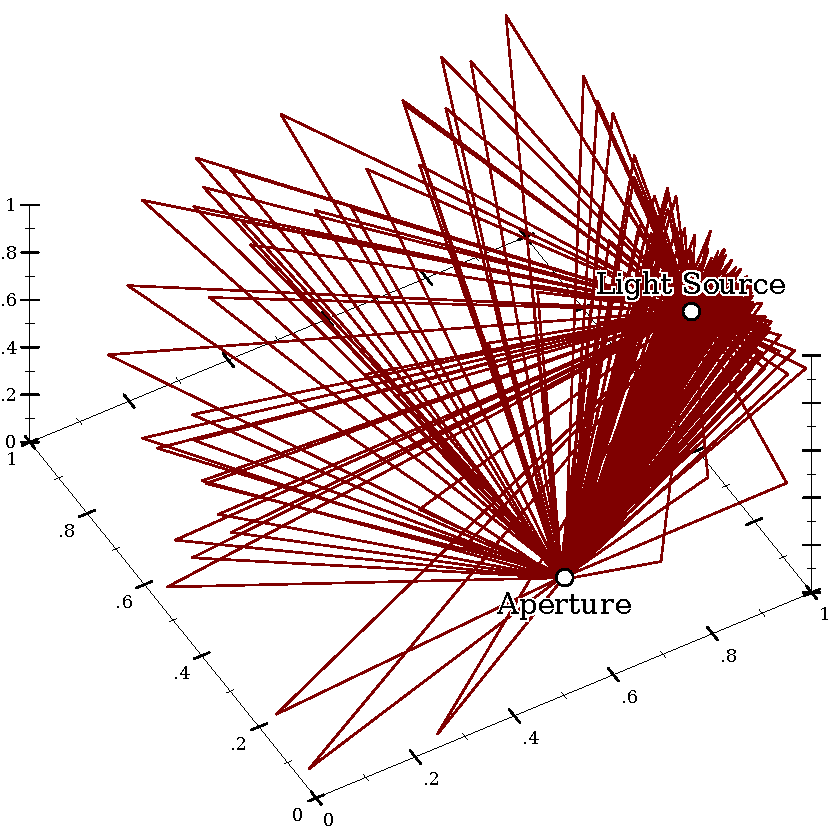
\includegraphics[width=\textwidth]{ray-tracing}
\end{minipage}
\label{fig:ray-tracing-paths}
}
\tab\tab
\subfloat[Random paths that pass through the aperture, projected onto a plane and accumulated.]{
\begin{minipage}{0.43\textwidth}
\centering
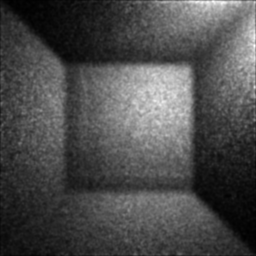
\includegraphics[width=\textwidth]{ray-tracing-projection}
\end{minipage}
\label{fig:ray-tracing-projection}
}

\subfloat[Part of the ray tracer implementation. Sampling involves computing approximate preimages under functions like this.]{
\usebox{\codebox}
\label{fig:ray-plane-intersect}
}
\caption[ ]{Stochastic ray tracing in Dr. Bayes is little more than physics simulation.}
\label{fig:ray-tracing}
\end{figure*}

\figref{fig:ray-tracing} shows the result of using Dr. Bayes for stochastic ray tracing~\cite{cit:veach-1997siggraph-mlt}.
In this instance, photons are cast from a light source in a uniformly random direction and are reflected by the walls of a square room, generating paths.
The objective is to sample, with the correct distribution, only those paths that pass through an aperture.
The smaller the aperture, the smaller the probability a path passes through it, and the more focused the resulting image.

All efficient implementations of stochastic ray tracing to date use sophisticated, specialized sampling methods that bear little resemblance to the physical processes they simulate.
The proof-of-concept ray tracer, written in Dr. Bayes, is little more than a simple physics simulation and a conditional query.


%%%%%%%%%%%%%%%%%%%%%%%%%%%%%%%%%%%%%%%%%%%%%%%%%%%%%%%%%%%%%%%%%%%%%%%%%%%%%%%%%%%%%%%%%%%%%%%%%%%%%
%%%%%%%%%%%%%%%%%%%%%%%%%%%%%%%%%%%%%%%%%%%%%%%%%%%%%%%%%%%%%%%%%%%%%%%%%%%%%%%%%%%%%%%%%%%%%%%%%%%%%
%%%%%%%%%%%%%%%%%%%%%%%%%%%%%%%%%%%%%%%%%%%%%%%%%%%%%%%%%%%%%%%%%%%%%%%%%%%%%%%%%%%%%%%%%%%%%%%%%%%%%

\section{Related Work}

Any programming language research described by the words ``bijective'' or ``reversible'' might seem to have much in common with ours.
Unfortunately, when we look more closely, we can usually draw only loose analogies and perhaps inspiration.
An example is lenses~\cite{cit:hofmann-2012popl-edit-lenses}, which are transformations from $X$ to $Y$ that can be run forward and backward, in a way that maintains some relationship between $X$ and $Y$.
Usually, a destructive, external process is assumed, so that, for example, a change from $y \in Y$ to $y' \in Y$ induces a corresponding change from $x \in X$ to some $x' \in X$.
When transformations lose information, lenses must satisfy certain behavioral laws.
In our work, no input or output is updated, and preimages are always definable regardless of non-injectivity.

Many multi-paradigm languages~\cite{cit:hanus-2007lp-multi-paradigm}, especially constraint functional languages, bear a strong resemblance to our work.
In fact, it is easy to add a $fail$ expression to our semantics, or to transform constraints into boolean program outputs.
The most obvious difference is evaluation strategy.
The most important difference is that our interpretation of programs returns \emph{distributions} of constrained outputs, rather than arbitrary single values that meet constraints.

The forward phase in computing preimages takes a subdomain and returns an overapproximation of the function's range for that subdomain.
This clearly generalizes interval arithmetic~\cite{cit:kearfott-1996eb-interval} to all first-order algebraic types.

Our approximating semantics can be regarded as an abstract interpretation~\cite{cit:cousot-1977popl-abstract-interpretation} where the concrete domain consists of measurable sets and the abstract domain consists of rectangular sets.
In some ways, it is quite typical: it is sound, it labels expressions, the abstract domain is a lattice, and the exact semantics it approximates performs infinite computations.
However, it is far from typical in other ways.
It is used to run programs, not for static analysis.
The abstraction boundaries are the $if$ branches of completely unrolled, infinite programs, and are not fixed.
There is no Kleene iteration.
Infinite computations are done in a library of \lzfclang-computable combinators, not by a semantic function.
This cleanly separates the syntax from the semantics, and allows us to prove the exact semantics correct mostly by proving simple categorical properties.

Probabilistic languages can be approximately placed into two groups: those defined by an implementation, and those defined by a semantics.

Some languages defined by an implementation are a probabilistic Scheme by Koller and Pfeffer~\cite{cit:koller-1997aaai-bayes-programs-short}, BUGS~\cite{cit:winbugs-language-short}, BLOG~\cite{cit:blog-language-short}, BLAISE~\cite{cit:blaise-language}, Church~\cite{cit:church-language-short}, and Kiselyov's embedded language for O'Caml based on continuations~\cite{cit:kiselyov-2008uai-monolingual}.
The reports on these languages generally describe interpreters, compilers, and algorithms for sampling with probabilistic conditions.
Recently, Wingate et al~\cite{cit:wingate-2011ais-lightweight,cit:wingate-2011nips-nonstandard} have defined the semantics of \emph{nonstandard interpretations} that enable efficient inference, but do not define the languages.

Early work in probabilistic language semantics is not motivated by Bayesian concerns, and thus does not address conditioning.
Kozen~\cite{cit:kozen-1979fcs-prob-programs-short} defines the meaning of bounded-space, imperative ``while'' programs as functions from probability measures to probability measures.
Hurd~\cite{cit:hurd-2002thesis} proves properties about programs with binary random choice by encoding programs and portions of measure theory in HOL.
Jones~\cite{cit:jones-1990thesis} develops a domain-theoretic variation of probability theory, and with it defines the probability monad, whose discrete version is a distribution-valued variation of the set or list monad.
Ramsey and Pfeffer~\cite{cit:ramsey-2002popl-stochastic-short} define the probability monad measure-theoretically and implement a language for finite probability.
Park~\cite{cit:park-2008toplas-prob} extends a $\lambda$-calculus with probabilistic choice from a general class of probability measures using inverse transform sampling.

Some recent work in probabilistic language semantics tackles conditioning. Pfeffer's IBAL~\cite{cit:pfeffer-2007chapter-ibal} is the earliest lambda calculus with finite probabilistic choice that also defines conditional queries.
Borgstr\"om et al~\cite{cit:borgstrom-2011esop-measure-transformer} develop Fun, a first-order functional language without recursion, extended with probabilistic choice and conditioning.
Its semantics interprets programs as \emph{measure transformers} by transforming expressions into arrow-like combinators.
The implementation generates a decomposition of the probability density represented by the program, if it exists.
Bhat et al~\cite{cit:bhat-2013etaps-densities} replaces Fun's $if$ with $match$, and interprets programs more directly as probability density functions by compositionally transforming expressions into an extension of the probability monad.


%%%%%%%%%%%%%%%%%%%%%%%%%%%%%%%%%%%%%%%%%%%%%%%%%%%%%%%%%%%%%%%%%%%%%%%%%%%%%%%%%%%%%%%%%%%%%%%%%%%%%
%%%%%%%%%%%%%%%%%%%%%%%%%%%%%%%%%%%%%%%%%%%%%%%%%%%%%%%%%%%%%%%%%%%%%%%%%%%%%%%%%%%%%%%%%%%%%%%%%%%%%
%%%%%%%%%%%%%%%%%%%%%%%%%%%%%%%%%%%%%%%%%%%%%%%%%%%%%%%%%%%%%%%%%%%%%%%%%%%%%%%%%%%%%%%%%%%%%%%%%%%%%

\section{Conclusions and Future Work}

To allow recursion and arbitrary conditions in probabilistic programs, we combined the power of measure theory with the unifying elegance of arrows. We
\begin{enumerate}
	\item Defined a transformation from first-order programs to arbitrary arrows.
	\item Defined the bottom arrow as a standard translation target.
	\item Derived the uncomputable preimage arrow as an alternative target.
	\item Derived a sound, computable approximation of the preimage arrow, and enough computable lifts to transform programs.
\end{enumerate}
Critically, the preimage arrow's lift from the bottom arrow distributes over bottom arrow computations.
Our semantics thus generalizes this process to all programs: 1) encode a program as a bottom arrow computation; 2) lift this computation to get an uncomputable function that computes preimages; 3) distribute the lift; and 4) replace uncomputable expressions with sound approximations.

Our semantics trades efficiency for simplicity by threading a constant, tree-shaped random source (Section~\ref{sec:threading-and-indexing}).
Passing subtrees instead would make $random$ a constant-time primitive, and allow combinators to detect lack of change and return cached values.
Other future optimization work includes creating new sampling algorithms, and using other easily measured but more expressive set representations, such as parallelotopes~\cite{cit:amato-2012tcs-parallelotopes}.
On the theory side, we intend to explore preimage computation's connection to type checking and type inference, investigate ways to integrate and leverage polymorphic type systems, and find the conditions under which preimage refinement is complete in the limit.

More broadly, we hope to advance Bayesian practice by providing a rich modeling language with an efficient, correct implementation, which allows general recursion and any computable, probabilistic condition.

%%%%%%%%%%%%%%%%%%%%%%%%%%%%%%%%%%%%%%%%%%%%%%%%%%%%%%%%%%%%%%%%%%%%%%%%%%%%%%%%%%%%%%%%%%%%%%%%%%%%%
%%%%%%%%%%%%%%%%%%%%%%%%%%%%%%%%%%%%%%%%%%%%%%%%%%%%%%%%%%%%%%%%%%%%%%%%%%%%%%%%%%%%%%%%%%%%%%%%%%%%%
%%%%%%%%%%%%%%%%%%%%%%%%%%%%%%%%%%%%%%%%%%%%%%%%%%%%%%%%%%%%%%%%%%%%%%%%%%%%%%%%%%%%%%%%%%%%%%%%%%%%%

\mathversion{normal}

%\appendix
%\section{Appendix Title}
%This is the text of the appendix, if you need one.

%\acks
%Acknowledgments, if needed.

\mathversion{normal}

\bibliographystyle{splncs03}
\bibliography{local-cites}

\end{document}
